\documentclass[twoside]{book}

% Packages required by doxygen
\usepackage{fixltx2e}
\usepackage{calc}
\usepackage{doxygen}
\usepackage{graphicx}
\usepackage[utf8]{inputenc}
\usepackage{makeidx}
\usepackage{multicol}
\usepackage{multirow}
\PassOptionsToPackage{warn}{textcomp}
\usepackage{textcomp}
\usepackage[nointegrals]{wasysym}
\usepackage[table]{xcolor}

% Font selection
\usepackage[T1]{fontenc}
\usepackage{mathptmx}
\usepackage[scaled=.90]{helvet}
\usepackage{courier}
\usepackage{amssymb}
\usepackage{sectsty}
\renewcommand{\familydefault}{\sfdefault}
\allsectionsfont{%
  \fontseries{bc}\selectfont%
  \color{darkgray}%
}
\renewcommand{\DoxyLabelFont}{%
  \fontseries{bc}\selectfont%
  \color{darkgray}%
}
\newcommand{\+}{\discretionary{\mbox{\scriptsize$\hookleftarrow$}}{}{}}

% Page & text layout
\usepackage{geometry}
\geometry{%
  a4paper,%
  top=2.5cm,%
  bottom=2.5cm,%
  left=2.5cm,%
  right=2.5cm%
}
\tolerance=750
\hfuzz=15pt
\hbadness=750
\setlength{\emergencystretch}{15pt}
\setlength{\parindent}{0cm}
\setlength{\parskip}{0.2cm}
\makeatletter
\renewcommand{\paragraph}{%
  \@startsection{paragraph}{4}{0ex}{-1.0ex}{1.0ex}{%
    \normalfont\normalsize\bfseries\SS@parafont%
  }%
}
\renewcommand{\subparagraph}{%
  \@startsection{subparagraph}{5}{0ex}{-1.0ex}{1.0ex}{%
    \normalfont\normalsize\bfseries\SS@subparafont%
  }%
}
\makeatother

% Headers & footers
\usepackage{fancyhdr}
\pagestyle{fancyplain}
\fancyhead[LE]{\fancyplain{}{\bfseries\thepage}}
\fancyhead[CE]{\fancyplain{}{}}
\fancyhead[RE]{\fancyplain{}{\bfseries\leftmark}}
\fancyhead[LO]{\fancyplain{}{\bfseries\rightmark}}
\fancyhead[CO]{\fancyplain{}{}}
\fancyhead[RO]{\fancyplain{}{\bfseries\thepage}}
\fancyfoot[LE]{\fancyplain{}{}}
\fancyfoot[CE]{\fancyplain{}{}}
\fancyfoot[RE]{\fancyplain{}{\bfseries\scriptsize Generated on Tue Dec 9 2014 13\+:28\+:52 for Ant\+Graphics by Doxygen }}
\fancyfoot[LO]{\fancyplain{}{\bfseries\scriptsize Generated on Tue Dec 9 2014 13\+:28\+:52 for Ant\+Graphics by Doxygen }}
\fancyfoot[CO]{\fancyplain{}{}}
\fancyfoot[RO]{\fancyplain{}{}}
\renewcommand{\footrulewidth}{0.4pt}
\renewcommand{\chaptermark}[1]{%
  \markboth{#1}{}%
}
\renewcommand{\sectionmark}[1]{%
  \markright{\thesection\ #1}%
}

% Indices & bibliography
\usepackage{natbib}
\usepackage[titles]{tocloft}
\setcounter{tocdepth}{3}
\setcounter{secnumdepth}{5}
\makeindex

% Hyperlinks (required, but should be loaded last)
\usepackage{ifpdf}
\ifpdf
  \usepackage[pdftex,pagebackref=true]{hyperref}
\else
  \usepackage[ps2pdf,pagebackref=true]{hyperref}
\fi
\hypersetup{%
  colorlinks=true,%
  linkcolor=blue,%
  citecolor=blue,%
  unicode%
}

% Custom commands
\newcommand{\clearemptydoublepage}{%
  \newpage{\pagestyle{empty}\cleardoublepage}%
}


%===== C O N T E N T S =====

\begin{document}

% Titlepage & ToC
\hypersetup{pageanchor=false,
             bookmarks=true,
             bookmarksnumbered=true,
             pdfencoding=unicode
            }
\pagenumbering{roman}
\begin{titlepage}
\vspace*{7cm}
\begin{center}%
{\Large Ant\+Graphics }\\
\vspace*{1cm}
{\large Generated by Doxygen 1.8.8}\\
\vspace*{0.5cm}
{\small Tue Dec 9 2014 13:28:52}\\
\end{center}
\end{titlepage}
\clearemptydoublepage
\tableofcontents
\clearemptydoublepage
\pagenumbering{arabic}
\hypersetup{pageanchor=true}

%--- Begin generated contents ---
\chapter{Hierarchical Index}
\section{Class Hierarchy}
This inheritance list is sorted roughly, but not completely, alphabetically\+:\begin{DoxyCompactList}
\item \contentsline{section}{ant\+Abstract\+App}{\pageref{classant_abstract_app}}{}
\item \contentsline{section}{ant\+Abtract\+Primitive}{\pageref{classant_abtract_primitive}}{}
\item \contentsline{section}{ant\+Camera}{\pageref{classant_camera}}{}
\item \contentsline{section}{ant\+Configuration}{\pageref{classant_configuration}}{}
\item \contentsline{section}{ant\+Drawable}{\pageref{classant_drawable}}{}
\begin{DoxyCompactList}
\item \contentsline{section}{ant\+Axis}{\pageref{classant_axis}}{}
\item \contentsline{section}{ant\+Cube}{\pageref{classant_cube}}{}
\begin{DoxyCompactList}
\item \contentsline{section}{ant\+Skybox}{\pageref{classant_skybox}}{}
\end{DoxyCompactList}
\item \contentsline{section}{ant\+Mesh}{\pageref{classant_mesh}}{}
\item \contentsline{section}{ant\+Plane}{\pageref{classant_plane}}{}
\item \contentsline{section}{ant\+Sphere}{\pageref{classant_sphere}}{}
\end{DoxyCompactList}
\item \contentsline{section}{ant\+Gui}{\pageref{classant_gui}}{}
\item \contentsline{section}{ant\+Material}{\pageref{classant_material}}{}
\item \contentsline{section}{ant\+Midi}{\pageref{classant_midi}}{}
\item \contentsline{section}{ant\+Obj\+Loader}{\pageref{classant_obj_loader}}{}
\item \contentsline{section}{ant\+Point\+Light}{\pageref{classant_point_light}}{}
\item \contentsline{section}{ant\+Shader}{\pageref{classant_shader}}{}
\item \contentsline{section}{ant\+Texture}{\pageref{classant_texture}}{}
\item \contentsline{section}{ant\+Vao}{\pageref{classant_vao}}{}
\item \contentsline{section}{ant\+Vbo}{\pageref{classant_vbo}}{}
\item \contentsline{section}{ant\+Window}{\pageref{classant_window}}{}
\item \contentsline{section}{mat3}{\pageref{structmat3}}{}
\item \contentsline{section}{mat4}{\pageref{structmat4}}{}
\item \contentsline{section}{vec2}{\pageref{structvec2}}{}
\item \contentsline{section}{vec3}{\pageref{structvec3}}{}
\item \contentsline{section}{vec4}{\pageref{structvec4}}{}
\item \contentsline{section}{versor}{\pageref{structversor}}{}
\end{DoxyCompactList}

\chapter{Class Index}
\section{Class List}
Here are the classes, structs, unions and interfaces with brief descriptions\+:\begin{DoxyCompactList}
\item\contentsline{section}{\hyperlink{classant_abstract_app}{ant\+Abstract\+App} \\*Abstract class for app definition }{\pageref{classant_abstract_app}}{}
\item\contentsline{section}{\hyperlink{classant_abstract_configuration}{ant\+Abstract\+Configuration} }{\pageref{classant_abstract_configuration}}{}
\item\contentsline{section}{\hyperlink{classant_abtract_primitive}{ant\+Abtract\+Primitive} }{\pageref{classant_abtract_primitive}}{}
\item\contentsline{section}{\hyperlink{classant_axis}{ant\+Axis} }{\pageref{classant_axis}}{}
\item\contentsline{section}{\hyperlink{classant_camera}{ant\+Camera} }{\pageref{classant_camera}}{}
\item\contentsline{section}{\hyperlink{classant_configuration}{ant\+Configuration} }{\pageref{classant_configuration}}{}
\item\contentsline{section}{\hyperlink{classant_cube}{ant\+Cube} }{\pageref{classant_cube}}{}
\item\contentsline{section}{\hyperlink{classant_drawable}{ant\+Drawable} }{\pageref{classant_drawable}}{}
\item\contentsline{section}{\hyperlink{classant_gui}{ant\+Gui} }{\pageref{classant_gui}}{}
\item\contentsline{section}{\hyperlink{classant_mapable_configuration}{ant\+Mapable\+Configuration} }{\pageref{classant_mapable_configuration}}{}
\item\contentsline{section}{\hyperlink{classant_mapable_material}{ant\+Mapable\+Material} }{\pageref{classant_mapable_material}}{}
\item\contentsline{section}{\hyperlink{classant_material}{ant\+Material} }{\pageref{classant_material}}{}
\item\contentsline{section}{\hyperlink{classant_mesh}{ant\+Mesh} }{\pageref{classant_mesh}}{}
\item\contentsline{section}{\hyperlink{classant_midi}{ant\+Midi} }{\pageref{classant_midi}}{}
\item\contentsline{section}{\hyperlink{classant_obj_loader}{ant\+Obj\+Loader} }{\pageref{classant_obj_loader}}{}
\item\contentsline{section}{\hyperlink{classant_plane}{ant\+Plane} }{\pageref{classant_plane}}{}
\item\contentsline{section}{\hyperlink{classant_point_light}{ant\+Point\+Light} }{\pageref{classant_point_light}}{}
\item\contentsline{section}{\hyperlink{classant_shader}{ant\+Shader} }{\pageref{classant_shader}}{}
\item\contentsline{section}{\hyperlink{classant_skybox}{ant\+Skybox} }{\pageref{classant_skybox}}{}
\item\contentsline{section}{\hyperlink{classant_sphere}{ant\+Sphere} }{\pageref{classant_sphere}}{}
\item\contentsline{section}{\hyperlink{classant_texture}{ant\+Texture} }{\pageref{classant_texture}}{}
\item\contentsline{section}{\hyperlink{classant_vao}{ant\+Vao} \\*Vertex array object }{\pageref{classant_vao}}{}
\item\contentsline{section}{\hyperlink{classant_vbo}{ant\+Vbo} \\*Vertex array object }{\pageref{classant_vbo}}{}
\item\contentsline{section}{\hyperlink{classant_window}{ant\+Window} \\*To define a glfw window with an opengl context }{\pageref{classant_window}}{}
\item\contentsline{section}{\hyperlink{structmat3}{mat3} }{\pageref{structmat3}}{}
\item\contentsline{section}{\hyperlink{structmat4}{mat4} }{\pageref{structmat4}}{}
\item\contentsline{section}{\hyperlink{structvec2}{vec2} }{\pageref{structvec2}}{}
\item\contentsline{section}{\hyperlink{structvec3}{vec3} }{\pageref{structvec3}}{}
\item\contentsline{section}{\hyperlink{structvec4}{vec4} }{\pageref{structvec4}}{}
\item\contentsline{section}{\hyperlink{structversor}{versor} }{\pageref{structversor}}{}
\end{DoxyCompactList}

\chapter{Class Documentation}
\hypertarget{classant_abstract_app}{\section{ant\+Abstract\+App Class Reference}
\label{classant_abstract_app}\index{ant\+Abstract\+App@{ant\+Abstract\+App}}
}


abstract class for app definition  




{\ttfamily \#include $<$ant\+Abstract\+App.\+h$>$}

\subsection*{Public Member Functions}
\begin{DoxyCompactItemize}
\item 
\hyperlink{classant_abstract_app_a5567c6adff87b08cb794565804325f6c}{$\sim$ant\+Abstract\+App} ()
\begin{DoxyCompactList}\small\item\em destructor \end{DoxyCompactList}\item 
virtual void \hyperlink{classant_abstract_app_a2e728002d7448d86eb81e2ffb272553e}{start} ()=0
\begin{DoxyCompactList}\small\item\em start app virtual method to init the app \end{DoxyCompactList}\item 
virtual void \hyperlink{classant_abstract_app_a19289810f175a2e19b90536a2a13a96e}{update} ()=0
\begin{DoxyCompactList}\small\item\em update app virtual method to update app attributes \end{DoxyCompactList}\item 
virtual void \hyperlink{classant_abstract_app_a52845a13d22bfc7ba426bc87c0f25cb5}{draw} ()=0
\begin{DoxyCompactList}\small\item\em draw virtual method to render the app \end{DoxyCompactList}\item 
virtual void \hyperlink{classant_abstract_app_ad27fa9b917e951470b6989ab015268c3}{shutdown} ()=0
\begin{DoxyCompactList}\small\item\em shutdown virtual method to clean the app \end{DoxyCompactList}\item 
double \hyperlink{classant_abstract_app_a0e7d74272d53e847e5fa6acc3d399e16}{get\+Current\+Time} ()
\end{DoxyCompactItemize}
\subsection*{Protected Member Functions}
\begin{DoxyCompactItemize}
\item 
\hyperlink{classant_abstract_app_ac1cbc2a3609ae4cde6ed6fc41af85d96}{ant\+Abstract\+App} (int window\+\_\+width, int window\+\_\+height, const std\+::string \&window\+\_\+title)
\begin{DoxyCompactList}\small\item\em constructor \end{DoxyCompactList}\item 
void \hyperlink{classant_abstract_app_a8fc3c5dcc8feb8ed8039afe41b1c63eb}{run} ()
\begin{DoxyCompactList}\small\item\em run the app \end{DoxyCompactList}\end{DoxyCompactItemize}
\subsection*{Protected Attributes}
\begin{DoxyCompactItemize}
\item 
ant\+Window\+Sh\+Ptr \hyperlink{classant_abstract_app_a2da8dc7071eb8f76ffe3fae6329439b2}{m\+\_\+window\+\_\+shptr}
\item 
double \hyperlink{classant_abstract_app_a3dd118d6793e653f1207abc4b498608d}{m\+\_\+mouse\+\_\+x\+\_\+pos}
\item 
double \hyperlink{classant_abstract_app_a44c5d57e580b3e68d076f638aa866bef}{m\+\_\+mouse\+\_\+y\+\_\+pos}
\item 
int \hyperlink{classant_abstract_app_a3346b67b4fe4b9627d9dbb064a08669b}{m\+\_\+frame\+\_\+count}
\item 
int \hyperlink{classant_abstract_app_a9d6e7846652cca2333831a19b1a4dad8}{m\+\_\+fps}
\item 
double \hyperlink{classant_abstract_app_a477dd78269fac0a6c2b20aa7fac41426}{m\+\_\+time}
\end{DoxyCompactItemize}
\subsection*{Private Member Functions}
\begin{DoxyCompactItemize}
\item 
int \hyperlink{classant_abstract_app_a205cc1e54945a8d88b270b0394958b3e}{update\+F\+P\+S\+Counter} ()
\begin{DoxyCompactList}\small\item\em update frame attributes \end{DoxyCompactList}\end{DoxyCompactItemize}


\subsection{Detailed Description}
abstract class for app definition 

class \hyperlink{classant_abstract_app}{ant\+Abstract\+App} 

\subsection{Constructor \& Destructor Documentation}
\hypertarget{classant_abstract_app_a5567c6adff87b08cb794565804325f6c}{\index{ant\+Abstract\+App@{ant\+Abstract\+App}!````~ant\+Abstract\+App@{$\sim$ant\+Abstract\+App}}
\index{````~ant\+Abstract\+App@{$\sim$ant\+Abstract\+App}!ant\+Abstract\+App@{ant\+Abstract\+App}}
\subsubsection[{$\sim$ant\+Abstract\+App}]{\setlength{\rightskip}{0pt plus 5cm}ant\+Abstract\+App\+::$\sim$ant\+Abstract\+App (
\begin{DoxyParamCaption}
{}
\end{DoxyParamCaption}
)}}\label{classant_abstract_app_a5567c6adff87b08cb794565804325f6c}


destructor 

$\sim$ant\+Abstract\+App \hypertarget{classant_abstract_app_ac1cbc2a3609ae4cde6ed6fc41af85d96}{\index{ant\+Abstract\+App@{ant\+Abstract\+App}!ant\+Abstract\+App@{ant\+Abstract\+App}}
\index{ant\+Abstract\+App@{ant\+Abstract\+App}!ant\+Abstract\+App@{ant\+Abstract\+App}}
\subsubsection[{ant\+Abstract\+App}]{\setlength{\rightskip}{0pt plus 5cm}ant\+Abstract\+App\+::ant\+Abstract\+App (
\begin{DoxyParamCaption}
\item[{int}]{window\+\_\+width, }
\item[{int}]{window\+\_\+height, }
\item[{const std\+::string \&}]{window\+\_\+title}
\end{DoxyParamCaption}
)\hspace{0.3cm}{\ttfamily [protected]}}}\label{classant_abstract_app_ac1cbc2a3609ae4cde6ed6fc41af85d96}


constructor 

\hyperlink{classant_abstract_app}{ant\+Abstract\+App} 
\begin{DoxyParams}{Parameters}
{\em window\+\_\+width} & window width \\
\hline
{\em window\+\_\+height} & window height \\
\hline
{\em window\+\_\+title} & window title \\
\hline
\end{DoxyParams}


\subsection{Member Function Documentation}
\hypertarget{classant_abstract_app_a52845a13d22bfc7ba426bc87c0f25cb5}{\index{ant\+Abstract\+App@{ant\+Abstract\+App}!draw@{draw}}
\index{draw@{draw}!ant\+Abstract\+App@{ant\+Abstract\+App}}
\subsubsection[{draw}]{\setlength{\rightskip}{0pt plus 5cm}virtual void ant\+Abstract\+App\+::draw (
\begin{DoxyParamCaption}
{}
\end{DoxyParamCaption}
)\hspace{0.3cm}{\ttfamily [pure virtual]}}}\label{classant_abstract_app_a52845a13d22bfc7ba426bc87c0f25cb5}


draw virtual method to render the app 

draw \hypertarget{classant_abstract_app_a0e7d74272d53e847e5fa6acc3d399e16}{\index{ant\+Abstract\+App@{ant\+Abstract\+App}!get\+Current\+Time@{get\+Current\+Time}}
\index{get\+Current\+Time@{get\+Current\+Time}!ant\+Abstract\+App@{ant\+Abstract\+App}}
\subsubsection[{get\+Current\+Time}]{\setlength{\rightskip}{0pt plus 5cm}double ant\+Abstract\+App\+::get\+Current\+Time (
\begin{DoxyParamCaption}
{}
\end{DoxyParamCaption}
)}}\label{classant_abstract_app_a0e7d74272d53e847e5fa6acc3d399e16}
get\+Current\+Time \begin{DoxyReturn}{Returns}
G\+L\+F\+W window time 
\end{DoxyReturn}
\hypertarget{classant_abstract_app_a8fc3c5dcc8feb8ed8039afe41b1c63eb}{\index{ant\+Abstract\+App@{ant\+Abstract\+App}!run@{run}}
\index{run@{run}!ant\+Abstract\+App@{ant\+Abstract\+App}}
\subsubsection[{run}]{\setlength{\rightskip}{0pt plus 5cm}void ant\+Abstract\+App\+::run (
\begin{DoxyParamCaption}
{}
\end{DoxyParamCaption}
)\hspace{0.3cm}{\ttfamily [protected]}}}\label{classant_abstract_app_a8fc3c5dcc8feb8ed8039afe41b1c63eb}


run the app 

run \hypertarget{classant_abstract_app_ad27fa9b917e951470b6989ab015268c3}{\index{ant\+Abstract\+App@{ant\+Abstract\+App}!shutdown@{shutdown}}
\index{shutdown@{shutdown}!ant\+Abstract\+App@{ant\+Abstract\+App}}
\subsubsection[{shutdown}]{\setlength{\rightskip}{0pt plus 5cm}virtual void ant\+Abstract\+App\+::shutdown (
\begin{DoxyParamCaption}
{}
\end{DoxyParamCaption}
)\hspace{0.3cm}{\ttfamily [pure virtual]}}}\label{classant_abstract_app_ad27fa9b917e951470b6989ab015268c3}


shutdown virtual method to clean the app 

shutdown \hypertarget{classant_abstract_app_a2e728002d7448d86eb81e2ffb272553e}{\index{ant\+Abstract\+App@{ant\+Abstract\+App}!start@{start}}
\index{start@{start}!ant\+Abstract\+App@{ant\+Abstract\+App}}
\subsubsection[{start}]{\setlength{\rightskip}{0pt plus 5cm}virtual void ant\+Abstract\+App\+::start (
\begin{DoxyParamCaption}
{}
\end{DoxyParamCaption}
)\hspace{0.3cm}{\ttfamily [pure virtual]}}}\label{classant_abstract_app_a2e728002d7448d86eb81e2ffb272553e}


start app virtual method to init the app 

start \hypertarget{classant_abstract_app_a19289810f175a2e19b90536a2a13a96e}{\index{ant\+Abstract\+App@{ant\+Abstract\+App}!update@{update}}
\index{update@{update}!ant\+Abstract\+App@{ant\+Abstract\+App}}
\subsubsection[{update}]{\setlength{\rightskip}{0pt plus 5cm}virtual void ant\+Abstract\+App\+::update (
\begin{DoxyParamCaption}
{}
\end{DoxyParamCaption}
)\hspace{0.3cm}{\ttfamily [pure virtual]}}}\label{classant_abstract_app_a19289810f175a2e19b90536a2a13a96e}


update app virtual method to update app attributes 

update \hypertarget{classant_abstract_app_a205cc1e54945a8d88b270b0394958b3e}{\index{ant\+Abstract\+App@{ant\+Abstract\+App}!update\+F\+P\+S\+Counter@{update\+F\+P\+S\+Counter}}
\index{update\+F\+P\+S\+Counter@{update\+F\+P\+S\+Counter}!ant\+Abstract\+App@{ant\+Abstract\+App}}
\subsubsection[{update\+F\+P\+S\+Counter}]{\setlength{\rightskip}{0pt plus 5cm}int ant\+Abstract\+App\+::update\+F\+P\+S\+Counter (
\begin{DoxyParamCaption}
{}
\end{DoxyParamCaption}
)\hspace{0.3cm}{\ttfamily [private]}}}\label{classant_abstract_app_a205cc1e54945a8d88b270b0394958b3e}


update frame attributes 

update\+F\+P\+S\+Counter \begin{DoxyReturn}{Returns}
current frame count 
\end{DoxyReturn}


\subsection{Member Data Documentation}
\hypertarget{classant_abstract_app_a9d6e7846652cca2333831a19b1a4dad8}{\index{ant\+Abstract\+App@{ant\+Abstract\+App}!m\+\_\+fps@{m\+\_\+fps}}
\index{m\+\_\+fps@{m\+\_\+fps}!ant\+Abstract\+App@{ant\+Abstract\+App}}
\subsubsection[{m\+\_\+fps}]{\setlength{\rightskip}{0pt plus 5cm}int ant\+Abstract\+App\+::m\+\_\+fps\hspace{0.3cm}{\ttfamily [protected]}}}\label{classant_abstract_app_a9d6e7846652cca2333831a19b1a4dad8}
current frame per seconds \hypertarget{classant_abstract_app_a3346b67b4fe4b9627d9dbb064a08669b}{\index{ant\+Abstract\+App@{ant\+Abstract\+App}!m\+\_\+frame\+\_\+count@{m\+\_\+frame\+\_\+count}}
\index{m\+\_\+frame\+\_\+count@{m\+\_\+frame\+\_\+count}!ant\+Abstract\+App@{ant\+Abstract\+App}}
\subsubsection[{m\+\_\+frame\+\_\+count}]{\setlength{\rightskip}{0pt plus 5cm}int ant\+Abstract\+App\+::m\+\_\+frame\+\_\+count\hspace{0.3cm}{\ttfamily [protected]}}}\label{classant_abstract_app_a3346b67b4fe4b9627d9dbb064a08669b}
current frame count \hypertarget{classant_abstract_app_a3dd118d6793e653f1207abc4b498608d}{\index{ant\+Abstract\+App@{ant\+Abstract\+App}!m\+\_\+mouse\+\_\+x\+\_\+pos@{m\+\_\+mouse\+\_\+x\+\_\+pos}}
\index{m\+\_\+mouse\+\_\+x\+\_\+pos@{m\+\_\+mouse\+\_\+x\+\_\+pos}!ant\+Abstract\+App@{ant\+Abstract\+App}}
\subsubsection[{m\+\_\+mouse\+\_\+x\+\_\+pos}]{\setlength{\rightskip}{0pt plus 5cm}double ant\+Abstract\+App\+::m\+\_\+mouse\+\_\+x\+\_\+pos\hspace{0.3cm}{\ttfamily [protected]}}}\label{classant_abstract_app_a3dd118d6793e653f1207abc4b498608d}
current mouse x position \hypertarget{classant_abstract_app_a44c5d57e580b3e68d076f638aa866bef}{\index{ant\+Abstract\+App@{ant\+Abstract\+App}!m\+\_\+mouse\+\_\+y\+\_\+pos@{m\+\_\+mouse\+\_\+y\+\_\+pos}}
\index{m\+\_\+mouse\+\_\+y\+\_\+pos@{m\+\_\+mouse\+\_\+y\+\_\+pos}!ant\+Abstract\+App@{ant\+Abstract\+App}}
\subsubsection[{m\+\_\+mouse\+\_\+y\+\_\+pos}]{\setlength{\rightskip}{0pt plus 5cm}double ant\+Abstract\+App\+::m\+\_\+mouse\+\_\+y\+\_\+pos\hspace{0.3cm}{\ttfamily [protected]}}}\label{classant_abstract_app_a44c5d57e580b3e68d076f638aa866bef}
current mouse y position \hypertarget{classant_abstract_app_a477dd78269fac0a6c2b20aa7fac41426}{\index{ant\+Abstract\+App@{ant\+Abstract\+App}!m\+\_\+time@{m\+\_\+time}}
\index{m\+\_\+time@{m\+\_\+time}!ant\+Abstract\+App@{ant\+Abstract\+App}}
\subsubsection[{m\+\_\+time}]{\setlength{\rightskip}{0pt plus 5cm}double ant\+Abstract\+App\+::m\+\_\+time\hspace{0.3cm}{\ttfamily [protected]}}}\label{classant_abstract_app_a477dd78269fac0a6c2b20aa7fac41426}
current time in seconds, updated each 0.\+25s \hypertarget{classant_abstract_app_a2da8dc7071eb8f76ffe3fae6329439b2}{\index{ant\+Abstract\+App@{ant\+Abstract\+App}!m\+\_\+window\+\_\+shptr@{m\+\_\+window\+\_\+shptr}}
\index{m\+\_\+window\+\_\+shptr@{m\+\_\+window\+\_\+shptr}!ant\+Abstract\+App@{ant\+Abstract\+App}}
\subsubsection[{m\+\_\+window\+\_\+shptr}]{\setlength{\rightskip}{0pt plus 5cm}ant\+Window\+Sh\+Ptr ant\+Abstract\+App\+::m\+\_\+window\+\_\+shptr\hspace{0.3cm}{\ttfamily [protected]}}}\label{classant_abstract_app_a2da8dc7071eb8f76ffe3fae6329439b2}
window 

The documentation for this class was generated from the following file\+:\begin{DoxyCompactItemize}
\item 
/\+Users/anthonycouret/\+Developer/ant\+Graphics/include/app/abstract/ant\+Abstract\+App.\+h\end{DoxyCompactItemize}

\hypertarget{classant_abstract_configuration}{\section{ant\+Abstract\+Configuration Class Reference}
\label{classant_abstract_configuration}\index{ant\+Abstract\+Configuration@{ant\+Abstract\+Configuration}}
}
Inheritance diagram for ant\+Abstract\+Configuration\+:\begin{figure}[H]
\begin{center}
\leavevmode
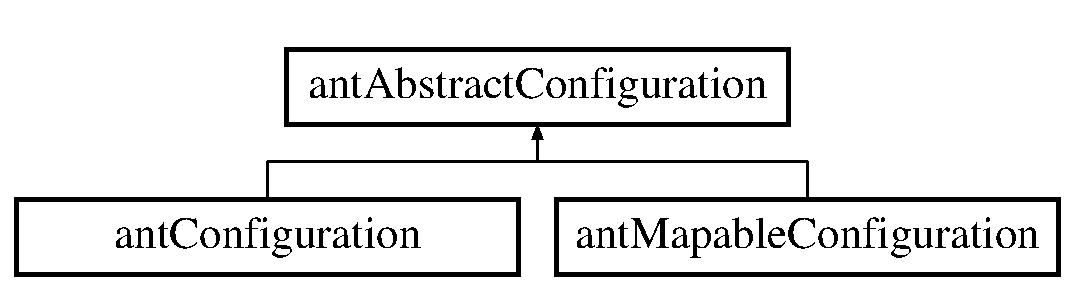
\includegraphics[height=2.000000cm]{classant_abstract_configuration}
\end{center}
\end{figure}
\subsection*{Public Member Functions}
\begin{DoxyCompactItemize}
\item 
virtual void \hyperlink{classant_abstract_configuration_a1c5fd57da800e0b5e0d6cd5fff2c6ca6}{set\+Position} (ant\+Vec3 position)=0
\begin{DoxyCompactList}\small\item\em position setter \end{DoxyCompactList}\item 
\hypertarget{classant_abstract_configuration_adef1a8c5835ba8af69a9d261e05c36d6}{virtual void {\bfseries set\+Rotation} (ant\+Quat rotation)=0}\label{classant_abstract_configuration_adef1a8c5835ba8af69a9d261e05c36d6}

\item 
\hypertarget{classant_abstract_configuration_a8ad082c6948d09574ee73655f2b4cfdb}{virtual void {\bfseries set\+Scale} (float scale)=0}\label{classant_abstract_configuration_a8ad082c6948d09574ee73655f2b4cfdb}

\item 
\hypertarget{classant_abstract_configuration_a642872fabf172c8cf01e13b3ca41681d}{virtual void {\bfseries set\+Type} (ant\+Rotation\+Type type)=0}\label{classant_abstract_configuration_a642872fabf172c8cf01e13b3ca41681d}

\item 
\hypertarget{classant_abstract_configuration_aa3aa7cfbaef8bd3aada4c67a64a31160}{virtual ant\+Mat4 {\bfseries get\+Local\+To\+World\+Matrix} ()=0}\label{classant_abstract_configuration_aa3aa7cfbaef8bd3aada4c67a64a31160}

\item 
\hypertarget{classant_abstract_configuration_a46effbdd3ec429e1616c4edcdff95fb8}{virtual ant\+Mat4 {\bfseries get\+World\+To\+Origin\+Matrix} ()=0}\label{classant_abstract_configuration_a46effbdd3ec429e1616c4edcdff95fb8}

\end{DoxyCompactItemize}


\subsection{Member Function Documentation}
\hypertarget{classant_abstract_configuration_a1c5fd57da800e0b5e0d6cd5fff2c6ca6}{\index{ant\+Abstract\+Configuration@{ant\+Abstract\+Configuration}!set\+Position@{set\+Position}}
\index{set\+Position@{set\+Position}!ant\+Abstract\+Configuration@{ant\+Abstract\+Configuration}}
\subsubsection[{set\+Position}]{\setlength{\rightskip}{0pt plus 5cm}virtual void ant\+Abstract\+Configuration\+::set\+Position (
\begin{DoxyParamCaption}
\item[{ant\+Vec3}]{position}
\end{DoxyParamCaption}
)\hspace{0.3cm}{\ttfamily [pure virtual]}}}\label{classant_abstract_configuration_a1c5fd57da800e0b5e0d6cd5fff2c6ca6}


position setter 

set\+Position 
\begin{DoxyParams}{Parameters}
{\em position} & position vector \\
\hline
\end{DoxyParams}


Implemented in \hyperlink{classant_configuration_af9a9ea5087d5179ebc2ff526a33a33e7}{ant\+Configuration}, and \hyperlink{classant_mapable_configuration_a0c868ba3a8773ad918d868fe0443f454}{ant\+Mapable\+Configuration}.



The documentation for this class was generated from the following file\+:\begin{DoxyCompactItemize}
\item 
/\+Users/anthonycouret/\+Developer/ant\+Graphics/include/configuration/ant\+Abstract\+Configuration.\+h\end{DoxyCompactItemize}

\hypertarget{classant_abtract_primitive}{\section{ant\+Abtract\+Primitive Class Reference}
\label{classant_abtract_primitive}\index{ant\+Abtract\+Primitive@{ant\+Abtract\+Primitive}}
}


The documentation for this class was generated from the following file\+:\begin{DoxyCompactItemize}
\item 
/\+Users/anthonycouret/\+Developer/ant\+Graphics/include/primitives/ant\+Abtract\+Primitive.\+h\end{DoxyCompactItemize}

\hypertarget{classant_axis}{\section{ant\+Axis Class Reference}
\label{classant_axis}\index{ant\+Axis@{ant\+Axis}}
}
Inheritance diagram for ant\+Axis\+:\begin{figure}[H]
\begin{center}
\leavevmode
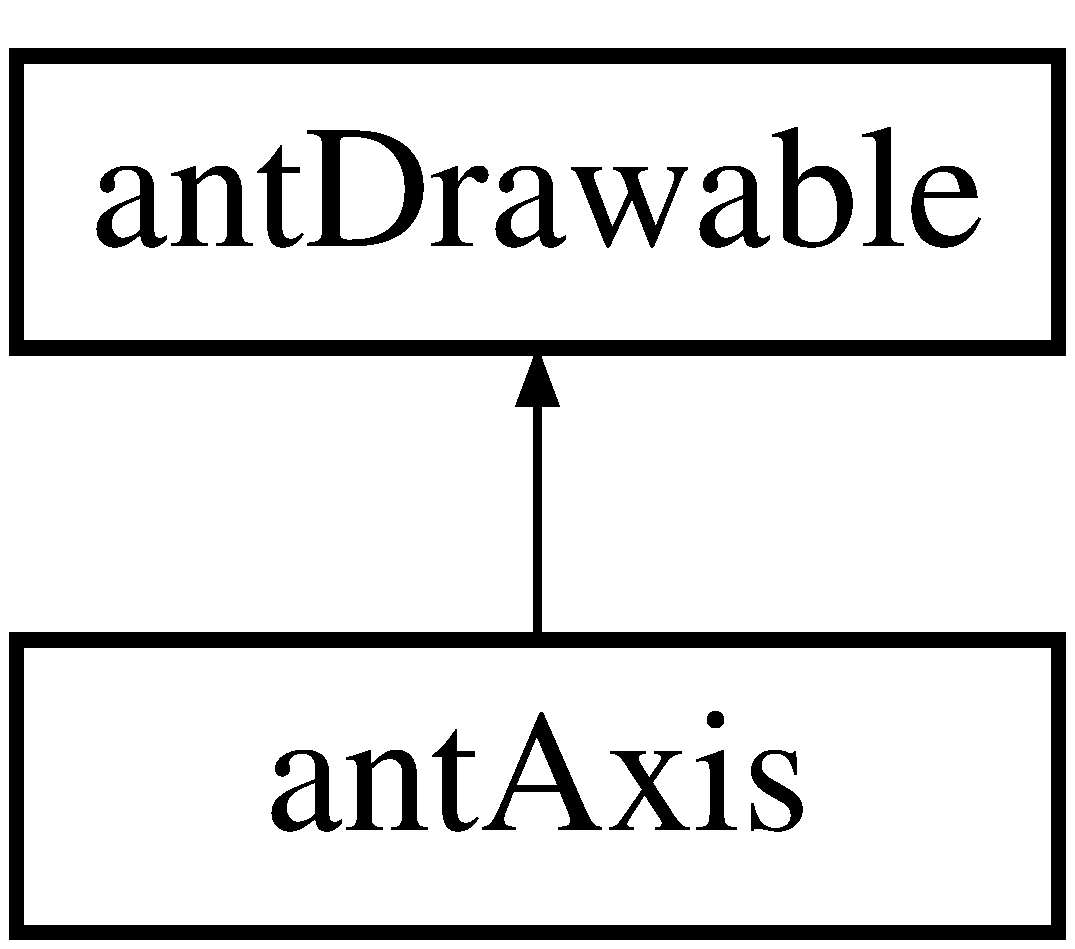
\includegraphics[height=2.000000cm]{classant_axis}
\end{center}
\end{figure}
\subsection*{Public Member Functions}
\begin{DoxyCompactItemize}
\item 
\hypertarget{classant_axis_ae50457cceb0427172e8036de339bc691}{void {\bfseries generate\+Vertices} ()}\label{classant_axis_ae50457cceb0427172e8036de339bc691}

\item 
\hypertarget{classant_axis_af82e81b2124b97373ecb5d9024ef1de0}{void {\bfseries generate\+Colors} ()}\label{classant_axis_af82e81b2124b97373ecb5d9024ef1de0}

\item 
\hypertarget{classant_axis_ae39f8df539511a5a0b06b5c81248ae2b}{virtual void {\bfseries draw} ()}\label{classant_axis_ae39f8df539511a5a0b06b5c81248ae2b}

\end{DoxyCompactItemize}
\subsection*{Static Public Member Functions}
\begin{DoxyCompactItemize}
\item 
\hypertarget{classant_axis_a372aa34f55e4b0050ff1a939087264ac}{static ant\+Axis\+Sh\+Ptr {\bfseries create} (int n\+Vbo, bool gen\+Colors=true)}\label{classant_axis_a372aa34f55e4b0050ff1a939087264ac}

\end{DoxyCompactItemize}
\subsection*{Private Member Functions}
\begin{DoxyCompactItemize}
\item 
\hypertarget{classant_axis_ad807544c38e19628d29eb336d61c417c}{{\bfseries ant\+Axis} (int n\+Vbo, bool gen\+Colors)}\label{classant_axis_ad807544c38e19628d29eb336d61c417c}

\end{DoxyCompactItemize}
\subsection*{Private Attributes}
\begin{DoxyCompactItemize}
\item 
\hypertarget{classant_axis_a2dc7112e89e7f094bca368b4c4437709}{ant\+Axis\+Wk\+Ptr {\bfseries m\+\_\+weak\+\_\+ptr}}\label{classant_axis_a2dc7112e89e7f094bca368b4c4437709}

\end{DoxyCompactItemize}
\subsection*{Additional Inherited Members}


The documentation for this class was generated from the following file\+:\begin{DoxyCompactItemize}
\item 
/\+Users/anthonycouret/\+Developer/ant\+Graphics/include/primitives/ant\+Axis.\+h\end{DoxyCompactItemize}

\hypertarget{classant_camera}{\section{ant\+Camera Class Reference}
\label{classant_camera}\index{ant\+Camera@{ant\+Camera}}
}
\subsection*{Public Member Functions}
\begin{DoxyCompactItemize}
\item 
\hypertarget{classant_camera_afc306c4adfde275b49c735ae68ee857e}{\hyperlink{structmat4}{mat4} {\bfseries get\+View\+Matrix} ()}\label{classant_camera_afc306c4adfde275b49c735ae68ee857e}

\item 
\hypertarget{classant_camera_a91398d63af3a186225ecb1d788b4b6d4}{\hyperlink{structmat4}{mat4} {\bfseries get\+Proj\+Matrix} ()}\label{classant_camera_a91398d63af3a186225ecb1d788b4b6d4}

\item 
\hypertarget{classant_camera_a02249b4eec2ba04abd37fe9ca24ddae5}{void {\bfseries set\+Position} (ant\+Vec3 position)}\label{classant_camera_a02249b4eec2ba04abd37fe9ca24ddae5}

\item 
\hypertarget{classant_camera_a2d05ef34b8057eaefd6a684d57cacbaa}{void {\bfseries set\+Rotation} (ant\+Quat rotation)}\label{classant_camera_a2d05ef34b8057eaefd6a684d57cacbaa}

\item 
\hypertarget{classant_camera_a155acb0975f1716f7e2d098799f59f6f}{void {\bfseries set\+Config\+Type} (bool type)}\label{classant_camera_a155acb0975f1716f7e2d098799f59f6f}

\end{DoxyCompactItemize}
\subsection*{Static Public Member Functions}
\begin{DoxyCompactItemize}
\item 
\hypertarget{classant_camera_ae545dc3467f359f7161f196cc84bf192}{static ant\+Camera\+Sh\+Ptr {\bfseries create} ()}\label{classant_camera_ae545dc3467f359f7161f196cc84bf192}

\end{DoxyCompactItemize}
\subsection*{Private Attributes}
\begin{DoxyCompactItemize}
\item 
\hypertarget{classant_camera_a29ecb5d46ef6f2bbd3adca58208c71c0}{float \hyperlink{classant_camera_a29ecb5d46ef6f2bbd3adca58208c71c0}{m\+\_\+near}}\label{classant_camera_a29ecb5d46ef6f2bbd3adca58208c71c0}

\begin{DoxyCompactList}\small\item\em near clipping plane \end{DoxyCompactList}\item 
\hypertarget{classant_camera_ad3f5a820c26d66965b42015f153dd868}{float \hyperlink{classant_camera_ad3f5a820c26d66965b42015f153dd868}{m\+\_\+far}}\label{classant_camera_ad3f5a820c26d66965b42015f153dd868}

\begin{DoxyCompactList}\small\item\em far clipping plane \end{DoxyCompactList}\item 
\hypertarget{classant_camera_adb5f87e2729f8dbc0a702f809982409f}{float \hyperlink{classant_camera_adb5f87e2729f8dbc0a702f809982409f}{m\+\_\+fov}}\label{classant_camera_adb5f87e2729f8dbc0a702f809982409f}

\begin{DoxyCompactList}\small\item\em field of view \end{DoxyCompactList}\item 
\hypertarget{classant_camera_a82f11705fc77ba2e86c667e31ea41e32}{float \hyperlink{classant_camera_a82f11705fc77ba2e86c667e31ea41e32}{m\+\_\+aspect\+\_\+ratio}}\label{classant_camera_a82f11705fc77ba2e86c667e31ea41e32}

\begin{DoxyCompactList}\small\item\em aspect ratio \end{DoxyCompactList}\item 
\hypertarget{classant_camera_a7807fb24803b6095cb9c19a067adcc9c}{ant\+Configuration\+Sh\+Ptr {\bfseries m\+\_\+world\+\_\+configuration}}\label{classant_camera_a7807fb24803b6095cb9c19a067adcc9c}

\item 
\hypertarget{classant_camera_a6ef6edf0c821f562036dd4294b8e1e57}{ant\+Camera\+Wk\+Ptr {\bfseries m\+\_\+weak\+\_\+ptr}}\label{classant_camera_a6ef6edf0c821f562036dd4294b8e1e57}

\end{DoxyCompactItemize}


The documentation for this class was generated from the following file\+:\begin{DoxyCompactItemize}
\item 
/\+Users/anthonycouret/\+Developer/ant\+\_\+graphics/ant\+\_\+graphics/include/camera/ant\+Camera.\+h\end{DoxyCompactItemize}

\hypertarget{classant_configuration}{\section{ant\+Configuration Class Reference}
\label{classant_configuration}\index{ant\+Configuration@{ant\+Configuration}}
}
Inheritance diagram for ant\+Configuration\+:\begin{figure}[H]
\begin{center}
\leavevmode
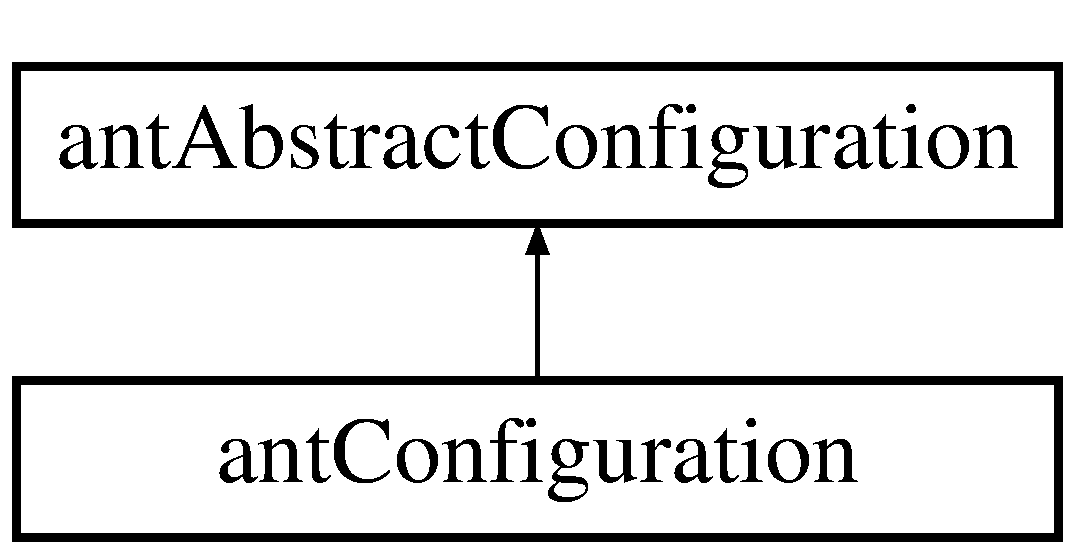
\includegraphics[height=2.000000cm]{classant_configuration}
\end{center}
\end{figure}
\subsection*{Public Member Functions}
\begin{DoxyCompactItemize}
\item 
\hyperlink{classant_configuration_a572b780d41fcc29ba89f8f43a719f1ae}{ant\+Configuration} (ant\+Rotation\+Type type)
\begin{DoxyCompactList}\small\item\em constructor \end{DoxyCompactList}\item 
virtual \hyperlink{classant_configuration_a76b24fe6a1488ac3d53bcb3292de9e41}{$\sim$ant\+Configuration} ()
\begin{DoxyCompactList}\small\item\em destructor \end{DoxyCompactList}\item 
virtual void \hyperlink{classant_configuration_af9a9ea5087d5179ebc2ff526a33a33e7}{set\+Position} (ant\+Vec3 position)
\begin{DoxyCompactList}\small\item\em position setter \end{DoxyCompactList}\item 
virtual void \hyperlink{classant_configuration_aef07bf707197372ffa3b454d0fa01b81}{set\+Rotation} (ant\+Quat rotation)
\begin{DoxyCompactList}\small\item\em rotation setter \end{DoxyCompactList}\item 
virtual void \hyperlink{classant_configuration_a85eb7a1ce3ad32a006aaae9a7b4d8991}{set\+Scale} (float scale)
\begin{DoxyCompactList}\small\item\em scale setter \end{DoxyCompactList}\item 
virtual void \hyperlink{classant_configuration_acb6ac97d627d528f5c3dbd5d7ef124b5}{set\+Type} (ant\+Rotation\+Type type)
\begin{DoxyCompactList}\small\item\em type setter \end{DoxyCompactList}\item 
ant\+Vec3 \hyperlink{classant_configuration_a4e178bdbab92eb1438b27d09a61bd2f3}{get\+Position} ()
\begin{DoxyCompactList}\small\item\em position getter \end{DoxyCompactList}\item 
ant\+Quat \hyperlink{classant_configuration_a88f393f030510d9893a7488c73332854}{get\+Rotation} ()
\begin{DoxyCompactList}\small\item\em rotation getter \end{DoxyCompactList}\item 
virtual ant\+Mat4 \hyperlink{classant_configuration_ad82e2e64fabdaf418b928c89c70cdd8a}{get\+Local\+To\+World\+Matrix} ()
\begin{DoxyCompactList}\small\item\em transform, rotate and scale identity matrix \end{DoxyCompactList}\item 
virtual ant\+Mat4 \hyperlink{classant_configuration_ac0a72cfaf4f48ee1671d917d12e5a686}{get\+World\+To\+Origin\+Matrix} ()
\begin{DoxyCompactList}\small\item\em inverse transform and rotate, then scale identity matrix \end{DoxyCompactList}\item 
\hypertarget{classant_configuration_a6edd6d57cd8f8ccb3545b91068ab5483}{ant\+Abstract\+Configuration\+Sh\+Ptr {\bfseries make\+Mapable} ()}\label{classant_configuration_a6edd6d57cd8f8ccb3545b91068ab5483}

\end{DoxyCompactItemize}
\subsection*{Static Public Member Functions}
\begin{DoxyCompactItemize}
\item 
static ant\+Configuration\+Sh\+Ptr \hyperlink{classant_configuration_a50a63e51ad01a040c130b9e729b1f47b}{create} (ant\+Rotation\+Type type=S\+E\+L\+F)
\begin{DoxyCompactList}\small\item\em static method to create an \hyperlink{classant_configuration}{ant\+Configuration} shared pointer \end{DoxyCompactList}\end{DoxyCompactItemize}
\subsection*{Private Attributes}
\begin{DoxyCompactItemize}
\item 
ant\+Rotation\+Type \hyperlink{classant_configuration_a9c6602c2995ea38583650da13b36b015}{m\+\_\+type}
\item 
ant\+Vec3 \hyperlink{classant_configuration_ab9fd2e843700f3589988064a9a2b494d}{m\+\_\+position}
\item 
ant\+Quat \hyperlink{classant_configuration_a2cd9ee51364f0481040a6c9c1faf42ac}{m\+\_\+rotation}
\item 
float \hyperlink{classant_configuration_ae1addd09ae683a014f37492aab019926}{m\+\_\+scale}
\item 
ant\+Configuration\+Wk\+Ptr \hyperlink{classant_configuration_a0ee5b6d1666f12fc211e274023780510}{m\+\_\+weak\+\_\+ptr}
\end{DoxyCompactItemize}


\subsection{Constructor \& Destructor Documentation}
\hypertarget{classant_configuration_a572b780d41fcc29ba89f8f43a719f1ae}{\index{ant\+Configuration@{ant\+Configuration}!ant\+Configuration@{ant\+Configuration}}
\index{ant\+Configuration@{ant\+Configuration}!ant\+Configuration@{ant\+Configuration}}
\subsubsection[{ant\+Configuration}]{\setlength{\rightskip}{0pt plus 5cm}ant\+Configuration\+::ant\+Configuration (
\begin{DoxyParamCaption}
\item[{ant\+Rotation\+Type}]{type}
\end{DoxyParamCaption}
)}}\label{classant_configuration_a572b780d41fcc29ba89f8f43a719f1ae}


constructor 

\hyperlink{classant_configuration}{ant\+Configuration} 
\begin{DoxyParams}{Parameters}
{\em type} & S\+E\+L\+F or O\+R\+B\+I\+T \\
\hline
\end{DoxyParams}
\hypertarget{classant_configuration_a76b24fe6a1488ac3d53bcb3292de9e41}{\index{ant\+Configuration@{ant\+Configuration}!````~ant\+Configuration@{$\sim$ant\+Configuration}}
\index{````~ant\+Configuration@{$\sim$ant\+Configuration}!ant\+Configuration@{ant\+Configuration}}
\subsubsection[{$\sim$ant\+Configuration}]{\setlength{\rightskip}{0pt plus 5cm}virtual ant\+Configuration\+::$\sim$ant\+Configuration (
\begin{DoxyParamCaption}
{}
\end{DoxyParamCaption}
)\hspace{0.3cm}{\ttfamily [virtual]}}}\label{classant_configuration_a76b24fe6a1488ac3d53bcb3292de9e41}


destructor 

$\sim$ant\+Configuration 

\subsection{Member Function Documentation}
\hypertarget{classant_configuration_a50a63e51ad01a040c130b9e729b1f47b}{\index{ant\+Configuration@{ant\+Configuration}!create@{create}}
\index{create@{create}!ant\+Configuration@{ant\+Configuration}}
\subsubsection[{create}]{\setlength{\rightskip}{0pt plus 5cm}static ant\+Configuration\+Sh\+Ptr ant\+Configuration\+::create (
\begin{DoxyParamCaption}
\item[{ant\+Rotation\+Type}]{type = {\ttfamily SELF}}
\end{DoxyParamCaption}
)\hspace{0.3cm}{\ttfamily [static]}}}\label{classant_configuration_a50a63e51ad01a040c130b9e729b1f47b}


static method to create an \hyperlink{classant_configuration}{ant\+Configuration} shared pointer 

create 
\begin{DoxyParams}{Parameters}
{\em type} & S\+E\+L\+F (default) or O\+R\+B\+I\+T\\
\hline
\end{DoxyParams}
\begin{DoxyReturn}{Returns}
an \hyperlink{classant_configuration}{ant\+Configuration} shared pointer 
\end{DoxyReturn}
\hypertarget{classant_configuration_ad82e2e64fabdaf418b928c89c70cdd8a}{\index{ant\+Configuration@{ant\+Configuration}!get\+Local\+To\+World\+Matrix@{get\+Local\+To\+World\+Matrix}}
\index{get\+Local\+To\+World\+Matrix@{get\+Local\+To\+World\+Matrix}!ant\+Configuration@{ant\+Configuration}}
\subsubsection[{get\+Local\+To\+World\+Matrix}]{\setlength{\rightskip}{0pt plus 5cm}virtual ant\+Mat4 ant\+Configuration\+::get\+Local\+To\+World\+Matrix (
\begin{DoxyParamCaption}
{}
\end{DoxyParamCaption}
)\hspace{0.3cm}{\ttfamily [virtual]}}}\label{classant_configuration_ad82e2e64fabdaf418b928c89c70cdd8a}


transform, rotate and scale identity matrix 

get\+Local\+To\+World\+Matrix \begin{DoxyReturn}{Returns}
local to world matrix 
\end{DoxyReturn}


Implements \hyperlink{classant_abstract_configuration}{ant\+Abstract\+Configuration}.

\hypertarget{classant_configuration_a4e178bdbab92eb1438b27d09a61bd2f3}{\index{ant\+Configuration@{ant\+Configuration}!get\+Position@{get\+Position}}
\index{get\+Position@{get\+Position}!ant\+Configuration@{ant\+Configuration}}
\subsubsection[{get\+Position}]{\setlength{\rightskip}{0pt plus 5cm}ant\+Vec3 ant\+Configuration\+::get\+Position (
\begin{DoxyParamCaption}
{}
\end{DoxyParamCaption}
)}}\label{classant_configuration_a4e178bdbab92eb1438b27d09a61bd2f3}


position getter 

get\+Position \begin{DoxyReturn}{Returns}
position vector 
\end{DoxyReturn}
\hypertarget{classant_configuration_a88f393f030510d9893a7488c73332854}{\index{ant\+Configuration@{ant\+Configuration}!get\+Rotation@{get\+Rotation}}
\index{get\+Rotation@{get\+Rotation}!ant\+Configuration@{ant\+Configuration}}
\subsubsection[{get\+Rotation}]{\setlength{\rightskip}{0pt plus 5cm}ant\+Quat ant\+Configuration\+::get\+Rotation (
\begin{DoxyParamCaption}
{}
\end{DoxyParamCaption}
)}}\label{classant_configuration_a88f393f030510d9893a7488c73332854}


rotation getter 

get\+Rotation \begin{DoxyReturn}{Returns}
rotation versor 
\end{DoxyReturn}
\hypertarget{classant_configuration_ac0a72cfaf4f48ee1671d917d12e5a686}{\index{ant\+Configuration@{ant\+Configuration}!get\+World\+To\+Origin\+Matrix@{get\+World\+To\+Origin\+Matrix}}
\index{get\+World\+To\+Origin\+Matrix@{get\+World\+To\+Origin\+Matrix}!ant\+Configuration@{ant\+Configuration}}
\subsubsection[{get\+World\+To\+Origin\+Matrix}]{\setlength{\rightskip}{0pt plus 5cm}virtual ant\+Mat4 ant\+Configuration\+::get\+World\+To\+Origin\+Matrix (
\begin{DoxyParamCaption}
{}
\end{DoxyParamCaption}
)\hspace{0.3cm}{\ttfamily [virtual]}}}\label{classant_configuration_ac0a72cfaf4f48ee1671d917d12e5a686}


inverse transform and rotate, then scale identity matrix 

get\+World\+To\+Origin\+Matrix \begin{DoxyReturn}{Returns}
world to origin matrix 
\end{DoxyReturn}


Implements \hyperlink{classant_abstract_configuration}{ant\+Abstract\+Configuration}.

\hypertarget{classant_configuration_af9a9ea5087d5179ebc2ff526a33a33e7}{\index{ant\+Configuration@{ant\+Configuration}!set\+Position@{set\+Position}}
\index{set\+Position@{set\+Position}!ant\+Configuration@{ant\+Configuration}}
\subsubsection[{set\+Position}]{\setlength{\rightskip}{0pt plus 5cm}virtual void ant\+Configuration\+::set\+Position (
\begin{DoxyParamCaption}
\item[{ant\+Vec3}]{position}
\end{DoxyParamCaption}
)\hspace{0.3cm}{\ttfamily [virtual]}}}\label{classant_configuration_af9a9ea5087d5179ebc2ff526a33a33e7}


position setter 

set\+Position set\+Position 
\begin{DoxyParams}{Parameters}
{\em position} & position vector \\
\hline
\end{DoxyParams}


Implements \hyperlink{classant_abstract_configuration_a1c5fd57da800e0b5e0d6cd5fff2c6ca6}{ant\+Abstract\+Configuration}.

\hypertarget{classant_configuration_aef07bf707197372ffa3b454d0fa01b81}{\index{ant\+Configuration@{ant\+Configuration}!set\+Rotation@{set\+Rotation}}
\index{set\+Rotation@{set\+Rotation}!ant\+Configuration@{ant\+Configuration}}
\subsubsection[{set\+Rotation}]{\setlength{\rightskip}{0pt plus 5cm}virtual void ant\+Configuration\+::set\+Rotation (
\begin{DoxyParamCaption}
\item[{ant\+Quat}]{rotation}
\end{DoxyParamCaption}
)\hspace{0.3cm}{\ttfamily [virtual]}}}\label{classant_configuration_aef07bf707197372ffa3b454d0fa01b81}


rotation setter 

set\+Rotation 
\begin{DoxyParams}{Parameters}
{\em rotation} & rotation versor \\
\hline
\end{DoxyParams}


Implements \hyperlink{classant_abstract_configuration}{ant\+Abstract\+Configuration}.

\hypertarget{classant_configuration_a85eb7a1ce3ad32a006aaae9a7b4d8991}{\index{ant\+Configuration@{ant\+Configuration}!set\+Scale@{set\+Scale}}
\index{set\+Scale@{set\+Scale}!ant\+Configuration@{ant\+Configuration}}
\subsubsection[{set\+Scale}]{\setlength{\rightskip}{0pt plus 5cm}virtual void ant\+Configuration\+::set\+Scale (
\begin{DoxyParamCaption}
\item[{float}]{scale}
\end{DoxyParamCaption}
)\hspace{0.3cm}{\ttfamily [virtual]}}}\label{classant_configuration_a85eb7a1ce3ad32a006aaae9a7b4d8991}


scale setter 

set\+Scale 
\begin{DoxyParams}{Parameters}
{\em scale} & scale factor \\
\hline
\end{DoxyParams}


Implements \hyperlink{classant_abstract_configuration}{ant\+Abstract\+Configuration}.

\hypertarget{classant_configuration_acb6ac97d627d528f5c3dbd5d7ef124b5}{\index{ant\+Configuration@{ant\+Configuration}!set\+Type@{set\+Type}}
\index{set\+Type@{set\+Type}!ant\+Configuration@{ant\+Configuration}}
\subsubsection[{set\+Type}]{\setlength{\rightskip}{0pt plus 5cm}virtual void ant\+Configuration\+::set\+Type (
\begin{DoxyParamCaption}
\item[{ant\+Rotation\+Type}]{type}
\end{DoxyParamCaption}
)\hspace{0.3cm}{\ttfamily [virtual]}}}\label{classant_configuration_acb6ac97d627d528f5c3dbd5d7ef124b5}


type setter 

set\+Type 
\begin{DoxyParams}{Parameters}
{\em type} & S\+E\+L\+F or O\+R\+B\+I\+T \\
\hline
\end{DoxyParams}


Implements \hyperlink{classant_abstract_configuration}{ant\+Abstract\+Configuration}.



\subsection{Member Data Documentation}
\hypertarget{classant_configuration_ab9fd2e843700f3589988064a9a2b494d}{\index{ant\+Configuration@{ant\+Configuration}!m\+\_\+position@{m\+\_\+position}}
\index{m\+\_\+position@{m\+\_\+position}!ant\+Configuration@{ant\+Configuration}}
\subsubsection[{m\+\_\+position}]{\setlength{\rightskip}{0pt plus 5cm}ant\+Vec3 ant\+Configuration\+::m\+\_\+position\hspace{0.3cm}{\ttfamily [private]}}}\label{classant_configuration_ab9fd2e843700f3589988064a9a2b494d}
position vector \hypertarget{classant_configuration_a2cd9ee51364f0481040a6c9c1faf42ac}{\index{ant\+Configuration@{ant\+Configuration}!m\+\_\+rotation@{m\+\_\+rotation}}
\index{m\+\_\+rotation@{m\+\_\+rotation}!ant\+Configuration@{ant\+Configuration}}
\subsubsection[{m\+\_\+rotation}]{\setlength{\rightskip}{0pt plus 5cm}ant\+Quat ant\+Configuration\+::m\+\_\+rotation\hspace{0.3cm}{\ttfamily [private]}}}\label{classant_configuration_a2cd9ee51364f0481040a6c9c1faf42ac}
rotation versor \hypertarget{classant_configuration_ae1addd09ae683a014f37492aab019926}{\index{ant\+Configuration@{ant\+Configuration}!m\+\_\+scale@{m\+\_\+scale}}
\index{m\+\_\+scale@{m\+\_\+scale}!ant\+Configuration@{ant\+Configuration}}
\subsubsection[{m\+\_\+scale}]{\setlength{\rightskip}{0pt plus 5cm}float ant\+Configuration\+::m\+\_\+scale\hspace{0.3cm}{\ttfamily [private]}}}\label{classant_configuration_ae1addd09ae683a014f37492aab019926}
scale factor \hypertarget{classant_configuration_a9c6602c2995ea38583650da13b36b015}{\index{ant\+Configuration@{ant\+Configuration}!m\+\_\+type@{m\+\_\+type}}
\index{m\+\_\+type@{m\+\_\+type}!ant\+Configuration@{ant\+Configuration}}
\subsubsection[{m\+\_\+type}]{\setlength{\rightskip}{0pt plus 5cm}ant\+Rotation\+Type ant\+Configuration\+::m\+\_\+type\hspace{0.3cm}{\ttfamily [private]}}}\label{classant_configuration_a9c6602c2995ea38583650da13b36b015}
rotation and transformation type \hypertarget{classant_configuration_a0ee5b6d1666f12fc211e274023780510}{\index{ant\+Configuration@{ant\+Configuration}!m\+\_\+weak\+\_\+ptr@{m\+\_\+weak\+\_\+ptr}}
\index{m\+\_\+weak\+\_\+ptr@{m\+\_\+weak\+\_\+ptr}!ant\+Configuration@{ant\+Configuration}}
\subsubsection[{m\+\_\+weak\+\_\+ptr}]{\setlength{\rightskip}{0pt plus 5cm}ant\+Configuration\+Wk\+Ptr ant\+Configuration\+::m\+\_\+weak\+\_\+ptr\hspace{0.3cm}{\ttfamily [private]}}}\label{classant_configuration_a0ee5b6d1666f12fc211e274023780510}
weak pointer 

The documentation for this class was generated from the following file\+:\begin{DoxyCompactItemize}
\item 
/\+Users/anthonycouret/\+Developer/ant\+Graphics/include/configuration/ant\+Configuration.\+h\end{DoxyCompactItemize}

\hypertarget{classant_cube}{\section{ant\+Cube Class Reference}
\label{classant_cube}\index{ant\+Cube@{ant\+Cube}}
}
Inheritance diagram for ant\+Cube\+:\begin{figure}[H]
\begin{center}
\leavevmode
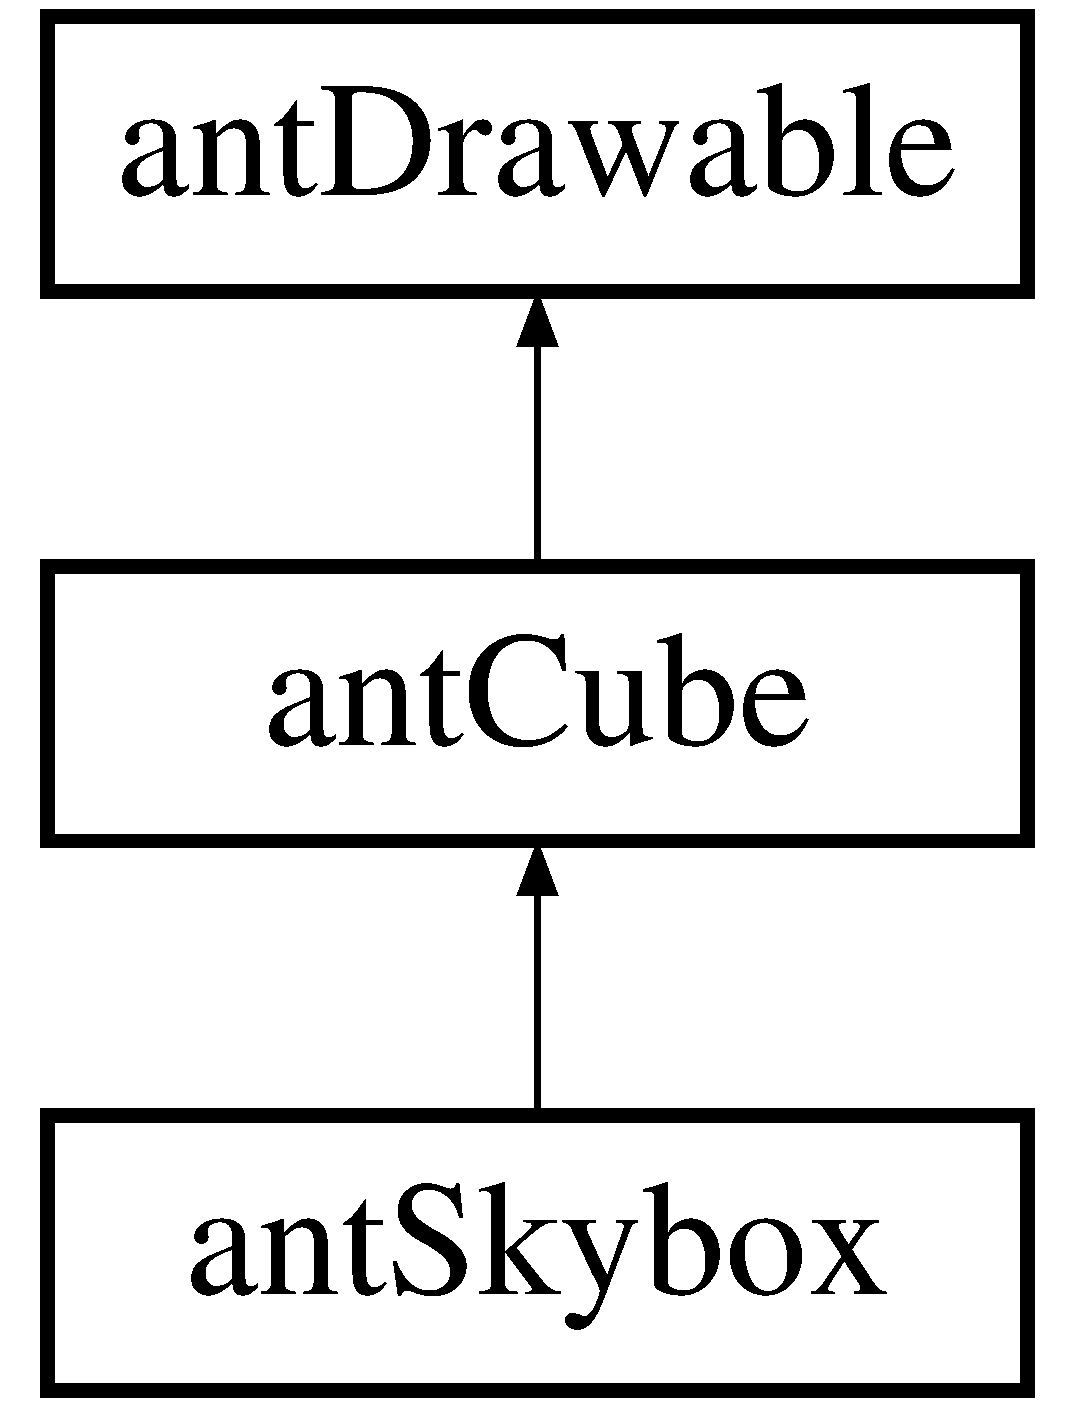
\includegraphics[height=3.000000cm]{classant_cube}
\end{center}
\end{figure}
\subsection*{Public Member Functions}
\begin{DoxyCompactItemize}
\item 
\hypertarget{classant_cube_a5d75beb683c2a6a654e040904c4096ac}{void {\bfseries generate\+Vertices} ()}\label{classant_cube_a5d75beb683c2a6a654e040904c4096ac}

\item 
\hypertarget{classant_cube_a5c962b1138474cfc40e05f2b4adab56e}{void {\bfseries generate\+Colors} ()}\label{classant_cube_a5c962b1138474cfc40e05f2b4adab56e}

\item 
\hypertarget{classant_cube_a284421916f0f30b8193aa23a7ad91734}{void {\bfseries generate\+Normals} ()}\label{classant_cube_a284421916f0f30b8193aa23a7ad91734}

\item 
\hypertarget{classant_cube_af838f52d1a949d1025ebf22f68717317}{void {\bfseries generate\+Tex\+Coords} ()}\label{classant_cube_af838f52d1a949d1025ebf22f68717317}

\item 
\hypertarget{classant_cube_a99eb2bdfb1895f984c7731c1e43aa767}{virtual void {\bfseries draw} ()}\label{classant_cube_a99eb2bdfb1895f984c7731c1e43aa767}

\end{DoxyCompactItemize}
\subsection*{Static Public Member Functions}
\begin{DoxyCompactItemize}
\item 
\hypertarget{classant_cube_a689b791b7ab0f1cd1de664e60fd3e393}{static ant\+Cube\+Sh\+Ptr {\bfseries create} (int n\+Vbo=4, bool gen\+Colors=true, bool gen\+Normals=true, bool gen\+Tex\+Coords=true)}\label{classant_cube_a689b791b7ab0f1cd1de664e60fd3e393}

\end{DoxyCompactItemize}
\subsection*{Protected Member Functions}
\begin{DoxyCompactItemize}
\item 
\hypertarget{classant_cube_ad2676f4b7c056e4158fb8a3e1ba98a23}{{\bfseries ant\+Cube} (int n\+Vbo, bool gen\+Colors, bool gen\+Normals, bool gen\+Tex\+Coords)}\label{classant_cube_ad2676f4b7c056e4158fb8a3e1ba98a23}

\end{DoxyCompactItemize}
\subsection*{Private Attributes}
\begin{DoxyCompactItemize}
\item 
\hypertarget{classant_cube_a9f9a444abfbd29f48ed66924c35083d3}{ant\+Cube\+Wk\+Ptr {\bfseries m\+\_\+weak\+\_\+ptr}}\label{classant_cube_a9f9a444abfbd29f48ed66924c35083d3}

\end{DoxyCompactItemize}
\subsection*{Additional Inherited Members}


The documentation for this class was generated from the following file\+:\begin{DoxyCompactItemize}
\item 
/\+Users/anthonycouret/\+Developer/ant\+\_\+graphics/ant\+\_\+graphics/include/primitives/ant\+Cube.\+h\end{DoxyCompactItemize}

\hypertarget{classant_drawable}{\section{ant\+Drawable Class Reference}
\label{classant_drawable}\index{ant\+Drawable@{ant\+Drawable}}
}
Inheritance diagram for ant\+Drawable\+:\begin{figure}[H]
\begin{center}
\leavevmode
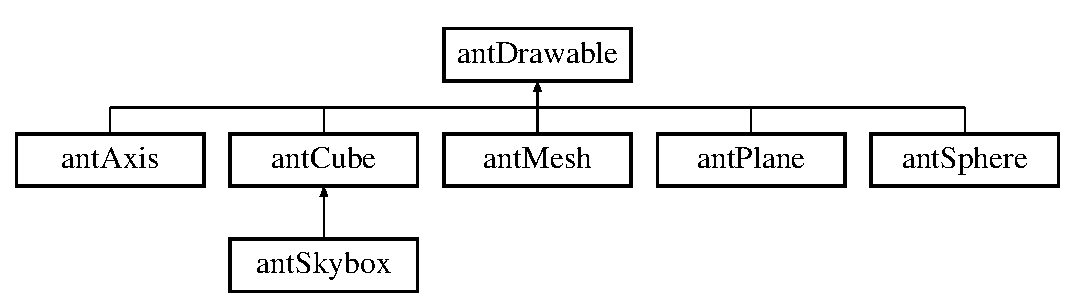
\includegraphics[height=3.000000cm]{classant_drawable}
\end{center}
\end{figure}
\subsection*{Public Member Functions}
\begin{DoxyCompactItemize}
\item 
\hypertarget{classant_drawable_a911b72e36adfdab82b5800c3da08f53d}{virtual void {\bfseries draw} (G\+Lenum mode, G\+Lboolean depth\+\_\+mask=G\+L\+\_\+\+T\+R\+U\+E)}\label{classant_drawable_a911b72e36adfdab82b5800c3da08f53d}

\item 
\hypertarget{classant_drawable_adb22318201dc679c672f3fa5b652a132}{void {\bfseries bind\+Vao} (int i)}\label{classant_drawable_adb22318201dc679c672f3fa5b652a132}

\item 
\hypertarget{classant_drawable_a5c7ff9f9339a47eda75cdfb93ee7813c}{void {\bfseries bind\+Vbo} (int i)}\label{classant_drawable_a5c7ff9f9339a47eda75cdfb93ee7813c}

\item 
\hypertarget{classant_drawable_a34c687f540d7577a16c84a57f2e2342b}{void {\bfseries set\+Data} (G\+Lsizeiptr size, const G\+Lvoid $\ast$data, G\+Lenum usage=G\+L\+\_\+\+S\+T\+A\+T\+I\+C\+\_\+\+D\+R\+A\+W)}\label{classant_drawable_a34c687f540d7577a16c84a57f2e2342b}

\item 
\hypertarget{classant_drawable_a0e41419e96b0f3d7832ea6d9dc568ee0}{void {\bfseries attrib} (G\+Luint index, G\+Lint size, G\+Lenum type=G\+L\+\_\+\+F\+L\+O\+A\+T, G\+Lboolean normalized=G\+L\+\_\+\+F\+A\+L\+S\+E, G\+Lsizei stride=0, const G\+Lvoid $\ast$pointer=0)}\label{classant_drawable_a0e41419e96b0f3d7832ea6d9dc568ee0}

\item 
\hypertarget{classant_drawable_a3de5a89016b2f1614153b31cd4ff8dd7}{int {\bfseries get\+N\+Vertices} () const }\label{classant_drawable_a3de5a89016b2f1614153b31cd4ff8dd7}

\item 
\hypertarget{classant_drawable_a13576b9816d01ed137c2ed246bd7edaa}{bool {\bfseries has\+Vertices} () const }\label{classant_drawable_a13576b9816d01ed137c2ed246bd7edaa}

\item 
\hypertarget{classant_drawable_ac30d77a790bed03e46e5f56365261860}{bool {\bfseries has\+Colors} () const }\label{classant_drawable_ac30d77a790bed03e46e5f56365261860}

\item 
\hypertarget{classant_drawable_aa7187bfae37caa0ff47f78c711c212ca}{bool {\bfseries has\+Normals} () const }\label{classant_drawable_aa7187bfae37caa0ff47f78c711c212ca}

\item 
\hypertarget{classant_drawable_af81901932344c894f3b4ec6fdf5bb71b}{bool {\bfseries has\+Tex\+Coords} () const }\label{classant_drawable_af81901932344c894f3b4ec6fdf5bb71b}

\item 
\hypertarget{classant_drawable_a04a5424888ad3629cbdc55d7e7f1c1c5}{void {\bfseries enable\+Vertices} ()}\label{classant_drawable_a04a5424888ad3629cbdc55d7e7f1c1c5}

\item 
\hypertarget{classant_drawable_abdf13d03cd40e156ce49a1d53e51e885}{void {\bfseries disable\+Vertices} ()}\label{classant_drawable_abdf13d03cd40e156ce49a1d53e51e885}

\item 
\hypertarget{classant_drawable_a4cac9be6832ab426de2415b2422324a2}{void {\bfseries enable\+Colors} ()}\label{classant_drawable_a4cac9be6832ab426de2415b2422324a2}

\item 
\hypertarget{classant_drawable_aea0eba49c2a15798a4841261127b1160}{void {\bfseries disable\+Colors} ()}\label{classant_drawable_aea0eba49c2a15798a4841261127b1160}

\item 
\hypertarget{classant_drawable_aa8054b4b43404e36107191a68b525848}{void {\bfseries enable\+Normals} ()}\label{classant_drawable_aa8054b4b43404e36107191a68b525848}

\item 
\hypertarget{classant_drawable_a9c137754de8ce180309fd4109ce5e934}{void {\bfseries disable\+Normals} ()}\label{classant_drawable_a9c137754de8ce180309fd4109ce5e934}

\item 
\hypertarget{classant_drawable_aa276fa4cbd827125bd864fa00f974cc4}{void {\bfseries enable\+Tex\+Coords} ()}\label{classant_drawable_aa276fa4cbd827125bd864fa00f974cc4}

\item 
\hypertarget{classant_drawable_a3e20a24ae16df52044e9dbb9c806083a}{void {\bfseries disable\+Tex\+Coords} ()}\label{classant_drawable_a3e20a24ae16df52044e9dbb9c806083a}

\item 
\hypertarget{classant_drawable_ad4a59354ce773bccf7ba5b9c949e1401}{void {\bfseries print} ()}\label{classant_drawable_ad4a59354ce773bccf7ba5b9c949e1401}

\item 
\hypertarget{classant_drawable_a1e176180c5d98f7d43863e1db51e9205}{void {\bfseries set\+Position} (ant\+Vec3 position)}\label{classant_drawable_a1e176180c5d98f7d43863e1db51e9205}

\item 
\hypertarget{classant_drawable_adfd3f1b5e87ea18fac525e08f28695e1}{void {\bfseries set\+Rotation} (ant\+Quat rotation)}\label{classant_drawable_adfd3f1b5e87ea18fac525e08f28695e1}

\item 
\hypertarget{classant_drawable_a714be84ca5ecf84989e273249d8be954}{void {\bfseries set\+Config\+Type} (bool type)}\label{classant_drawable_a714be84ca5ecf84989e273249d8be954}

\item 
\hypertarget{classant_drawable_ab666efd2bca92495cce545977cd9e2b6}{void {\bfseries set\+Scale} (float scale)}\label{classant_drawable_ab666efd2bca92495cce545977cd9e2b6}

\item 
\hypertarget{classant_drawable_a128866275b3cead6d1a7224eddf7d9b6}{ant\+Mat4 {\bfseries get\+Model\+Matrix} ()}\label{classant_drawable_a128866275b3cead6d1a7224eddf7d9b6}

\end{DoxyCompactItemize}
\subsection*{Protected Member Functions}
\begin{DoxyCompactItemize}
\item 
\hypertarget{classant_drawable_af4a5b1c438c6e057e3579479a51ec220}{{\bfseries ant\+Drawable} (int n\+Vbo,...)}\label{classant_drawable_af4a5b1c438c6e057e3579479a51ec220}

\end{DoxyCompactItemize}
\subsection*{Protected Attributes}
\begin{DoxyCompactItemize}
\item 
\hypertarget{classant_drawable_a44467c7a66f32ecc52de456ec65d4ecf}{ant\+Vao\+Sh\+Ptr {\bfseries m\+\_\+vao}}\label{classant_drawable_a44467c7a66f32ecc52de456ec65d4ecf}

\item 
\hypertarget{classant_drawable_a115e4aa45582fefe01f5fd7e8ba81c1c}{ant\+Vbo\+Sh\+Ptr {\bfseries m\+\_\+vbo}}\label{classant_drawable_a115e4aa45582fefe01f5fd7e8ba81c1c}

\item 
\hypertarget{classant_drawable_a00f537df3d1eed56d18c41f21f77dd4c}{int {\bfseries m\+\_\+n\+Vertices}}\label{classant_drawable_a00f537df3d1eed56d18c41f21f77dd4c}

\item 
\hypertarget{classant_drawable_afd6edb277d05fd04e633b8f7e8918f18}{G\+Lfloat $\ast$ {\bfseries m\+\_\+vertices}}\label{classant_drawable_afd6edb277d05fd04e633b8f7e8918f18}

\item 
\hypertarget{classant_drawable_a289640b95bc5e0a5a3965788945c27c3}{bool {\bfseries m\+\_\+has\+Vertices}}\label{classant_drawable_a289640b95bc5e0a5a3965788945c27c3}

\item 
\hypertarget{classant_drawable_a4ad2abc29a7bb97094f94917971ece04}{bool {\bfseries m\+\_\+vertices\+Enabled}}\label{classant_drawable_a4ad2abc29a7bb97094f94917971ece04}

\item 
\hypertarget{classant_drawable_a9cd5939ef8624ce765cadded921a8e6e}{G\+Lfloat $\ast$ {\bfseries m\+\_\+colors}}\label{classant_drawable_a9cd5939ef8624ce765cadded921a8e6e}

\item 
\hypertarget{classant_drawable_a554bfc525b6cb26d6c33fc7176b96596}{bool {\bfseries m\+\_\+has\+Colors}}\label{classant_drawable_a554bfc525b6cb26d6c33fc7176b96596}

\item 
\hypertarget{classant_drawable_addcb899b2071b0b87e2aa21f86873425}{bool {\bfseries m\+\_\+colors\+Enabled}}\label{classant_drawable_addcb899b2071b0b87e2aa21f86873425}

\item 
\hypertarget{classant_drawable_a43c390b562c431ded8b76f5ddba2ff03}{G\+Lfloat $\ast$ {\bfseries m\+\_\+normals}}\label{classant_drawable_a43c390b562c431ded8b76f5ddba2ff03}

\item 
\hypertarget{classant_drawable_a34f05f633360395ad6f9d8c524b92737}{bool {\bfseries m\+\_\+has\+Normals}}\label{classant_drawable_a34f05f633360395ad6f9d8c524b92737}

\item 
\hypertarget{classant_drawable_a77369a2341dcf92011260f57f5d86aec}{bool {\bfseries m\+\_\+normals\+Enabled}}\label{classant_drawable_a77369a2341dcf92011260f57f5d86aec}

\item 
\hypertarget{classant_drawable_af1cb237b3861412af1e8ec5519b36d73}{G\+Lfloat $\ast$ {\bfseries m\+\_\+texcoords}}\label{classant_drawable_af1cb237b3861412af1e8ec5519b36d73}

\item 
\hypertarget{classant_drawable_ab8dfeca134b6d453375cc86f17962d39}{bool {\bfseries m\+\_\+has\+Tex\+Coords}}\label{classant_drawable_ab8dfeca134b6d453375cc86f17962d39}

\item 
\hypertarget{classant_drawable_a7fa69da9f4ceb1134858b561521b16fd}{bool {\bfseries m\+\_\+texcoords\+Enabled}}\label{classant_drawable_a7fa69da9f4ceb1134858b561521b16fd}

\item 
\hypertarget{classant_drawable_abb81baba7f4269a61e0cb7fc000cd7c6}{ant\+Configuration\+Sh\+Ptr {\bfseries m\+\_\+world\+\_\+config}}\label{classant_drawable_abb81baba7f4269a61e0cb7fc000cd7c6}

\end{DoxyCompactItemize}


The documentation for this class was generated from the following file\+:\begin{DoxyCompactItemize}
\item 
/\+Users/anthonycouret/\+Developer/ant\+\_\+graphics/ant\+\_\+graphics/include/gl/ant\+Drawable.\+h\end{DoxyCompactItemize}

\hypertarget{classant_gui}{\section{ant\+Gui Class Reference}
\label{classant_gui}\index{ant\+Gui@{ant\+Gui}}
}
\subsection*{Public Member Functions}
\begin{DoxyCompactItemize}
\item 
\hypertarget{classant_gui_af5ac8a7bc1dba022721abb5bf0abacf4}{void {\bfseries draw} ()}\label{classant_gui_af5ac8a7bc1dba022721abb5bf0abacf4}

\item 
\hypertarget{classant_gui_a9adcce1fff8441b8df983579e20eba70}{int {\bfseries add\+Bar} (const std\+::string \&name)}\label{classant_gui_a9adcce1fff8441b8df983579e20eba70}

\item 
\hypertarget{classant_gui_a8d04951cf76d44d6f7bc93daac2ac760}{void {\bfseries add\+R\+G\+B\+A\+Var\+R\+W} (int bar\+\_\+id, const std\+::string \&name, ant\+R\+G\+B\+A $\ast$var)}\label{classant_gui_a8d04951cf76d44d6f7bc93daac2ac760}

\item 
\hypertarget{classant_gui_a9da1d56f2ddff3f65ed49161d8a20605}{void {\bfseries add\+Quat\+Var\+R\+W} (int bar\+\_\+id, const std\+::string \&name, ant\+Vec4 $\ast$var)}\label{classant_gui_a9da1d56f2ddff3f65ed49161d8a20605}

\item 
\hypertarget{classant_gui_af60ea51ab6b08de2e19f23703211409f}{void {\bfseries add\+Vec3\+Var\+R\+W} (int bar\+\_\+id, const std\+::string \&name, ant\+Vec3 $\ast$var)}\label{classant_gui_af60ea51ab6b08de2e19f23703211409f}

\item 
\hypertarget{classant_gui_a83e8eb1ff5c1c2f93e1a1fb3e3cbba6e}{void {\bfseries add\+Toggle\+R\+W} (int bar\+\_\+id, const std\+::string \&name, bool $\ast$var)}\label{classant_gui_a83e8eb1ff5c1c2f93e1a1fb3e3cbba6e}

\item 
\hypertarget{classant_gui_aa2b6c03e320d06935f88eb3ba72a9a29}{void {\bfseries def\+Var\+Short\+Cut} (int bar\+\_\+id, const std\+::string \&name, const std\+::string \&incr\+Key, const std\+::string \&decr\+Key)}\label{classant_gui_aa2b6c03e320d06935f88eb3ba72a9a29}

\end{DoxyCompactItemize}
\subsection*{Static Public Member Functions}
\begin{DoxyCompactItemize}
\item 
\hypertarget{classant_gui_aa847c3474231b558d26e1cf1f9fe4f91}{static ant\+Gui\+Sh\+Ptr {\bfseries create} (ant\+Window\+Sh\+Ptr window)}\label{classant_gui_aa847c3474231b558d26e1cf1f9fe4f91}

\item 
\hypertarget{classant_gui_a3bfa2b7f8c6b4fcf5ec8304dff581617}{static void {\bfseries Tw\+Event\+Mouse\+Button\+G\+L\+F\+W3} (G\+L\+F\+Wwindow $\ast$window, int button, int action, int mods)}\label{classant_gui_a3bfa2b7f8c6b4fcf5ec8304dff581617}

\item 
\hypertarget{classant_gui_abe31b4c0947f0910aa884c1be833f721}{static void {\bfseries Tw\+Event\+Mouse\+Pos\+G\+L\+F\+W3} (G\+L\+F\+Wwindow $\ast$window, double xpos, double ypos)}\label{classant_gui_abe31b4c0947f0910aa884c1be833f721}

\item 
\hypertarget{classant_gui_a8a046204e11b5274d11e3e6a45ea6d20}{static void {\bfseries Tw\+Event\+Mouse\+Wheel\+G\+L\+F\+W3} (G\+L\+F\+Wwindow $\ast$window, double xoffset, double yoffset)}\label{classant_gui_a8a046204e11b5274d11e3e6a45ea6d20}

\item 
\hypertarget{classant_gui_a3f2370a3570eddf3a5c8344cc99f5dbf}{static void {\bfseries Tw\+Event\+Key\+G\+L\+F\+W3} (G\+L\+F\+Wwindow $\ast$window, int key, int scancode, int action, int mods)}\label{classant_gui_a3f2370a3570eddf3a5c8344cc99f5dbf}

\item 
\hypertarget{classant_gui_a13477eb70c741334289ccd2d8a932cfa}{static void {\bfseries Tw\+Event\+Char\+G\+L\+F\+W3} (G\+L\+F\+Wwindow $\ast$window, int codepoint)}\label{classant_gui_a13477eb70c741334289ccd2d8a932cfa}

\item 
\hypertarget{classant_gui_a3f2322380ca04b7f8494057751a1fe9e}{static void {\bfseries Tw\+Window\+Size\+G\+L\+F\+W3} (G\+L\+F\+Wwindow $\ast$window, int width, int height)}\label{classant_gui_a3f2322380ca04b7f8494057751a1fe9e}

\end{DoxyCompactItemize}
\subsection*{Private Member Functions}
\begin{DoxyCompactItemize}
\item 
\hypertarget{classant_gui_ab6adc95e908a4402d7d5fade947d67f2}{{\bfseries ant\+Gui} (ant\+Window\+Sh\+Ptr window)}\label{classant_gui_ab6adc95e908a4402d7d5fade947d67f2}

\end{DoxyCompactItemize}
\subsection*{Private Attributes}
\begin{DoxyCompactItemize}
\item 
\hypertarget{classant_gui_adf2f6e372b6dc46315d66531edf6179f}{int {\bfseries m\+\_\+bars\+\_\+count}}\label{classant_gui_adf2f6e372b6dc46315d66531edf6179f}

\item 
\hypertarget{classant_gui_a4f83fb0fdc6e4f2aa3a2112b3dc23444}{std\+::vector$<$ Tw\+Bar $\ast$ $>$ {\bfseries m\+\_\+ant\+\_\+bars}}\label{classant_gui_a4f83fb0fdc6e4f2aa3a2112b3dc23444}

\item 
\hypertarget{classant_gui_a33923e64b3106da222d90d70bc5b4eec}{std\+::vector$<$ std\+::string $>$ {\bfseries m\+\_\+bar\+\_\+names}}\label{classant_gui_a33923e64b3106da222d90d70bc5b4eec}

\item 
\hypertarget{classant_gui_a0725f279e92c15c3dbf01b222bba1907}{ant\+Gui\+Wk\+Ptr {\bfseries m\+\_\+weak\+\_\+ptr}}\label{classant_gui_a0725f279e92c15c3dbf01b222bba1907}

\end{DoxyCompactItemize}


The documentation for this class was generated from the following file\+:\begin{DoxyCompactItemize}
\item 
/\+Users/anthonycouret/\+Developer/ant\+\_\+graphics/ant\+\_\+graphics/include/gui/ant\+Gui.\+h\end{DoxyCompactItemize}

\hypertarget{classant_mapable_configuration}{\section{ant\+Mapable\+Configuration Class Reference}
\label{classant_mapable_configuration}\index{ant\+Mapable\+Configuration@{ant\+Mapable\+Configuration}}
}
Inheritance diagram for ant\+Mapable\+Configuration\+:\begin{figure}[H]
\begin{center}
\leavevmode
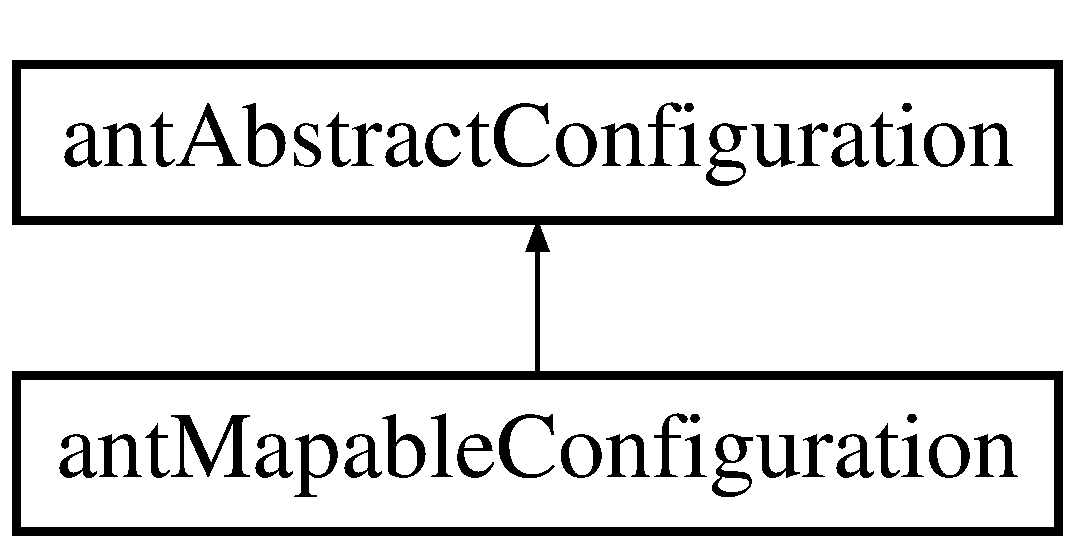
\includegraphics[height=2.000000cm]{classant_mapable_configuration}
\end{center}
\end{figure}
\subsection*{Public Member Functions}
\begin{DoxyCompactItemize}
\item 
\hypertarget{classant_mapable_configuration_a2617ce19af5d343f72205f74a764bcd7}{{\bfseries ant\+Mapable\+Configuration} (ant\+Rotation\+Type type)}\label{classant_mapable_configuration_a2617ce19af5d343f72205f74a764bcd7}

\item 
virtual \hyperlink{classant_mapable_configuration_ae8a4e2e32f16d82307d698526eeaa3d2}{$\sim$ant\+Mapable\+Configuration} ()
\begin{DoxyCompactList}\small\item\em destructor \end{DoxyCompactList}\item 
virtual void \hyperlink{classant_mapable_configuration_a0c868ba3a8773ad918d868fe0443f454}{set\+Position} (ant\+Vec3 position)
\begin{DoxyCompactList}\small\item\em position setter \end{DoxyCompactList}\item 
virtual void \hyperlink{classant_mapable_configuration_aface0ddcf2b7b664d95182a6ef3bb49f}{set\+Rotation} (ant\+Quat rotation)
\begin{DoxyCompactList}\small\item\em rotation setter \end{DoxyCompactList}\item 
virtual void \hyperlink{classant_mapable_configuration_a548a00bee9290bd14419d46a56609f13}{set\+Scale} (float scale)
\begin{DoxyCompactList}\small\item\em scale setter \end{DoxyCompactList}\item 
virtual void \hyperlink{classant_mapable_configuration_a2976225cdfb5febabd7374b742aec8db}{set\+Type} (ant\+Rotation\+Type type)
\begin{DoxyCompactList}\small\item\em type setter \end{DoxyCompactList}\item 
ant\+Mapable\+Vec3 \hyperlink{classant_mapable_configuration_ad7ca2e5ed86e3f7f9e08b25e41c8178f}{get\+Mapable\+Position} ()
\begin{DoxyCompactList}\small\item\em position pointer getter \end{DoxyCompactList}\item 
ant\+Mapable\+Quat \hyperlink{classant_mapable_configuration_ae7ceaa2c58d0538666bd73960cf4f8e4}{get\+Mapable\+Rotation} ()
\begin{DoxyCompactList}\small\item\em rotation getter \end{DoxyCompactList}\item 
\hypertarget{classant_mapable_configuration_a6071febe811791e1aa53c91e2d5be30d}{ant\+Mapable\+Vec4 {\bfseries get\+Tw\+Mapable\+Rotation} ()}\label{classant_mapable_configuration_a6071febe811791e1aa53c91e2d5be30d}

\item 
virtual ant\+Mat4 \hyperlink{classant_mapable_configuration_a5c9a9abf15b45ad0f6851dc3caf20342}{get\+Local\+To\+World\+Matrix} ()
\begin{DoxyCompactList}\small\item\em transform, rotate and scale identity matrix \end{DoxyCompactList}\item 
virtual ant\+Mat4 \hyperlink{classant_mapable_configuration_ac46245a2ba3b704309a85412c16d73ba}{get\+World\+To\+Origin\+Matrix} ()
\begin{DoxyCompactList}\small\item\em inverse transform and rotate, then scale identity matrix \end{DoxyCompactList}\item 
\hypertarget{classant_mapable_configuration_a0c4195ffdb71966119ebdea8ef5a46e6}{ant\+Abstract\+Configuration\+Sh\+Ptr {\bfseries make\+Base} ()}\label{classant_mapable_configuration_a0c4195ffdb71966119ebdea8ef5a46e6}

\end{DoxyCompactItemize}
\subsection*{Static Public Member Functions}
\begin{DoxyCompactItemize}
\item 
\hypertarget{classant_mapable_configuration_a32f253dd6ace10a4956a113d21f85666}{static ant\+Mapable\+Configuration\+Sh\+Ptr {\bfseries create} (ant\+Rotation\+Type type=S\+E\+L\+F)}\label{classant_mapable_configuration_a32f253dd6ace10a4956a113d21f85666}

\end{DoxyCompactItemize}
\subsection*{Private Attributes}
\begin{DoxyCompactItemize}
\item 
ant\+Mapable\+Rot\+Type \hyperlink{classant_mapable_configuration_abf6ce9445acae576092246c9bfeade86}{m\+\_\+type}
\item 
ant\+Mapable\+Vec3 \hyperlink{classant_mapable_configuration_aa6407ddaead7f445d696d91ab7c736ed}{m\+\_\+position}
\item 
ant\+Mapable\+Quat \hyperlink{classant_mapable_configuration_a14ba37effab1c8341a75c6362cd2def4}{m\+\_\+rotation}
\item 
\hypertarget{classant_mapable_configuration_aa831622293bb88a5c13d79e457a78a33}{ant\+Mapable\+Vec4 {\bfseries m\+\_\+tw\+\_\+rotation}}\label{classant_mapable_configuration_aa831622293bb88a5c13d79e457a78a33}

\item 
ant\+Mapable\+Float \hyperlink{classant_mapable_configuration_af0954326d95c30af4f04c473fc830569}{m\+\_\+scale}
\item 
ant\+Mapable\+Configuration\+Wk\+Ptr \hyperlink{classant_mapable_configuration_a4e41179ff8075a4d8834e4151bbd7fdb}{m\+\_\+weak\+\_\+ptr}
\end{DoxyCompactItemize}


\subsection{Constructor \& Destructor Documentation}
\hypertarget{classant_mapable_configuration_ae8a4e2e32f16d82307d698526eeaa3d2}{\index{ant\+Mapable\+Configuration@{ant\+Mapable\+Configuration}!````~ant\+Mapable\+Configuration@{$\sim$ant\+Mapable\+Configuration}}
\index{````~ant\+Mapable\+Configuration@{$\sim$ant\+Mapable\+Configuration}!ant\+Mapable\+Configuration@{ant\+Mapable\+Configuration}}
\subsubsection[{$\sim$ant\+Mapable\+Configuration}]{\setlength{\rightskip}{0pt plus 5cm}virtual ant\+Mapable\+Configuration\+::$\sim$ant\+Mapable\+Configuration (
\begin{DoxyParamCaption}
{}
\end{DoxyParamCaption}
)\hspace{0.3cm}{\ttfamily [virtual]}}}\label{classant_mapable_configuration_ae8a4e2e32f16d82307d698526eeaa3d2}


destructor 

$\sim$ant\+Mapable\+Configuration 

\subsection{Member Function Documentation}
\hypertarget{classant_mapable_configuration_a5c9a9abf15b45ad0f6851dc3caf20342}{\index{ant\+Mapable\+Configuration@{ant\+Mapable\+Configuration}!get\+Local\+To\+World\+Matrix@{get\+Local\+To\+World\+Matrix}}
\index{get\+Local\+To\+World\+Matrix@{get\+Local\+To\+World\+Matrix}!ant\+Mapable\+Configuration@{ant\+Mapable\+Configuration}}
\subsubsection[{get\+Local\+To\+World\+Matrix}]{\setlength{\rightskip}{0pt plus 5cm}virtual ant\+Mat4 ant\+Mapable\+Configuration\+::get\+Local\+To\+World\+Matrix (
\begin{DoxyParamCaption}
{}
\end{DoxyParamCaption}
)\hspace{0.3cm}{\ttfamily [virtual]}}}\label{classant_mapable_configuration_a5c9a9abf15b45ad0f6851dc3caf20342}


transform, rotate and scale identity matrix 

get\+Local\+To\+World\+Matrix \begin{DoxyReturn}{Returns}
local to world matrix 
\end{DoxyReturn}


Implements \hyperlink{classant_abstract_configuration}{ant\+Abstract\+Configuration}.

\hypertarget{classant_mapable_configuration_ad7ca2e5ed86e3f7f9e08b25e41c8178f}{\index{ant\+Mapable\+Configuration@{ant\+Mapable\+Configuration}!get\+Mapable\+Position@{get\+Mapable\+Position}}
\index{get\+Mapable\+Position@{get\+Mapable\+Position}!ant\+Mapable\+Configuration@{ant\+Mapable\+Configuration}}
\subsubsection[{get\+Mapable\+Position}]{\setlength{\rightskip}{0pt plus 5cm}ant\+Mapable\+Vec3 ant\+Mapable\+Configuration\+::get\+Mapable\+Position (
\begin{DoxyParamCaption}
{}
\end{DoxyParamCaption}
)}}\label{classant_mapable_configuration_ad7ca2e5ed86e3f7f9e08b25e41c8178f}


position pointer getter 

get\+Mapable\+Position \begin{DoxyReturn}{Returns}
position vector pointer 
\end{DoxyReturn}
\hypertarget{classant_mapable_configuration_ae7ceaa2c58d0538666bd73960cf4f8e4}{\index{ant\+Mapable\+Configuration@{ant\+Mapable\+Configuration}!get\+Mapable\+Rotation@{get\+Mapable\+Rotation}}
\index{get\+Mapable\+Rotation@{get\+Mapable\+Rotation}!ant\+Mapable\+Configuration@{ant\+Mapable\+Configuration}}
\subsubsection[{get\+Mapable\+Rotation}]{\setlength{\rightskip}{0pt plus 5cm}ant\+Mapable\+Quat ant\+Mapable\+Configuration\+::get\+Mapable\+Rotation (
\begin{DoxyParamCaption}
{}
\end{DoxyParamCaption}
)}}\label{classant_mapable_configuration_ae7ceaa2c58d0538666bd73960cf4f8e4}


rotation getter 

get\+Rotation \begin{DoxyReturn}{Returns}
rotation versor 
\end{DoxyReturn}
\hypertarget{classant_mapable_configuration_ac46245a2ba3b704309a85412c16d73ba}{\index{ant\+Mapable\+Configuration@{ant\+Mapable\+Configuration}!get\+World\+To\+Origin\+Matrix@{get\+World\+To\+Origin\+Matrix}}
\index{get\+World\+To\+Origin\+Matrix@{get\+World\+To\+Origin\+Matrix}!ant\+Mapable\+Configuration@{ant\+Mapable\+Configuration}}
\subsubsection[{get\+World\+To\+Origin\+Matrix}]{\setlength{\rightskip}{0pt plus 5cm}virtual ant\+Mat4 ant\+Mapable\+Configuration\+::get\+World\+To\+Origin\+Matrix (
\begin{DoxyParamCaption}
{}
\end{DoxyParamCaption}
)\hspace{0.3cm}{\ttfamily [virtual]}}}\label{classant_mapable_configuration_ac46245a2ba3b704309a85412c16d73ba}


inverse transform and rotate, then scale identity matrix 

get\+World\+To\+Origin\+Matrix \begin{DoxyReturn}{Returns}
world to origin matrix 
\end{DoxyReturn}


Implements \hyperlink{classant_abstract_configuration}{ant\+Abstract\+Configuration}.

\hypertarget{classant_mapable_configuration_a0c868ba3a8773ad918d868fe0443f454}{\index{ant\+Mapable\+Configuration@{ant\+Mapable\+Configuration}!set\+Position@{set\+Position}}
\index{set\+Position@{set\+Position}!ant\+Mapable\+Configuration@{ant\+Mapable\+Configuration}}
\subsubsection[{set\+Position}]{\setlength{\rightskip}{0pt plus 5cm}virtual void ant\+Mapable\+Configuration\+::set\+Position (
\begin{DoxyParamCaption}
\item[{ant\+Vec3}]{position}
\end{DoxyParamCaption}
)\hspace{0.3cm}{\ttfamily [virtual]}}}\label{classant_mapable_configuration_a0c868ba3a8773ad918d868fe0443f454}


position setter 

set\+Position 
\begin{DoxyParams}{Parameters}
{\em position} & position vector \\
\hline
\end{DoxyParams}


Implements \hyperlink{classant_abstract_configuration_a1c5fd57da800e0b5e0d6cd5fff2c6ca6}{ant\+Abstract\+Configuration}.

\hypertarget{classant_mapable_configuration_aface0ddcf2b7b664d95182a6ef3bb49f}{\index{ant\+Mapable\+Configuration@{ant\+Mapable\+Configuration}!set\+Rotation@{set\+Rotation}}
\index{set\+Rotation@{set\+Rotation}!ant\+Mapable\+Configuration@{ant\+Mapable\+Configuration}}
\subsubsection[{set\+Rotation}]{\setlength{\rightskip}{0pt plus 5cm}virtual void ant\+Mapable\+Configuration\+::set\+Rotation (
\begin{DoxyParamCaption}
\item[{ant\+Quat}]{rotation}
\end{DoxyParamCaption}
)\hspace{0.3cm}{\ttfamily [virtual]}}}\label{classant_mapable_configuration_aface0ddcf2b7b664d95182a6ef3bb49f}


rotation setter 

set\+Rotation 
\begin{DoxyParams}{Parameters}
{\em rotation} & rotation versor \\
\hline
\end{DoxyParams}


Implements \hyperlink{classant_abstract_configuration}{ant\+Abstract\+Configuration}.

\hypertarget{classant_mapable_configuration_a548a00bee9290bd14419d46a56609f13}{\index{ant\+Mapable\+Configuration@{ant\+Mapable\+Configuration}!set\+Scale@{set\+Scale}}
\index{set\+Scale@{set\+Scale}!ant\+Mapable\+Configuration@{ant\+Mapable\+Configuration}}
\subsubsection[{set\+Scale}]{\setlength{\rightskip}{0pt plus 5cm}virtual void ant\+Mapable\+Configuration\+::set\+Scale (
\begin{DoxyParamCaption}
\item[{float}]{scale}
\end{DoxyParamCaption}
)\hspace{0.3cm}{\ttfamily [virtual]}}}\label{classant_mapable_configuration_a548a00bee9290bd14419d46a56609f13}


scale setter 

set\+Scale 
\begin{DoxyParams}{Parameters}
{\em scale} & scale factor \\
\hline
\end{DoxyParams}


Implements \hyperlink{classant_abstract_configuration}{ant\+Abstract\+Configuration}.

\hypertarget{classant_mapable_configuration_a2976225cdfb5febabd7374b742aec8db}{\index{ant\+Mapable\+Configuration@{ant\+Mapable\+Configuration}!set\+Type@{set\+Type}}
\index{set\+Type@{set\+Type}!ant\+Mapable\+Configuration@{ant\+Mapable\+Configuration}}
\subsubsection[{set\+Type}]{\setlength{\rightskip}{0pt plus 5cm}virtual void ant\+Mapable\+Configuration\+::set\+Type (
\begin{DoxyParamCaption}
\item[{ant\+Rotation\+Type}]{type}
\end{DoxyParamCaption}
)\hspace{0.3cm}{\ttfamily [virtual]}}}\label{classant_mapable_configuration_a2976225cdfb5febabd7374b742aec8db}


type setter 

set\+Type 
\begin{DoxyParams}{Parameters}
{\em type} & S\+E\+L\+F or O\+R\+B\+I\+T \\
\hline
\end{DoxyParams}


Implements \hyperlink{classant_abstract_configuration}{ant\+Abstract\+Configuration}.



\subsection{Member Data Documentation}
\hypertarget{classant_mapable_configuration_aa6407ddaead7f445d696d91ab7c736ed}{\index{ant\+Mapable\+Configuration@{ant\+Mapable\+Configuration}!m\+\_\+position@{m\+\_\+position}}
\index{m\+\_\+position@{m\+\_\+position}!ant\+Mapable\+Configuration@{ant\+Mapable\+Configuration}}
\subsubsection[{m\+\_\+position}]{\setlength{\rightskip}{0pt plus 5cm}ant\+Mapable\+Vec3 ant\+Mapable\+Configuration\+::m\+\_\+position\hspace{0.3cm}{\ttfamily [private]}}}\label{classant_mapable_configuration_aa6407ddaead7f445d696d91ab7c736ed}
position vector \hypertarget{classant_mapable_configuration_a14ba37effab1c8341a75c6362cd2def4}{\index{ant\+Mapable\+Configuration@{ant\+Mapable\+Configuration}!m\+\_\+rotation@{m\+\_\+rotation}}
\index{m\+\_\+rotation@{m\+\_\+rotation}!ant\+Mapable\+Configuration@{ant\+Mapable\+Configuration}}
\subsubsection[{m\+\_\+rotation}]{\setlength{\rightskip}{0pt plus 5cm}ant\+Mapable\+Quat ant\+Mapable\+Configuration\+::m\+\_\+rotation\hspace{0.3cm}{\ttfamily [private]}}}\label{classant_mapable_configuration_a14ba37effab1c8341a75c6362cd2def4}
rotation versor \hypertarget{classant_mapable_configuration_af0954326d95c30af4f04c473fc830569}{\index{ant\+Mapable\+Configuration@{ant\+Mapable\+Configuration}!m\+\_\+scale@{m\+\_\+scale}}
\index{m\+\_\+scale@{m\+\_\+scale}!ant\+Mapable\+Configuration@{ant\+Mapable\+Configuration}}
\subsubsection[{m\+\_\+scale}]{\setlength{\rightskip}{0pt plus 5cm}ant\+Mapable\+Float ant\+Mapable\+Configuration\+::m\+\_\+scale\hspace{0.3cm}{\ttfamily [private]}}}\label{classant_mapable_configuration_af0954326d95c30af4f04c473fc830569}
scale factor \hypertarget{classant_mapable_configuration_abf6ce9445acae576092246c9bfeade86}{\index{ant\+Mapable\+Configuration@{ant\+Mapable\+Configuration}!m\+\_\+type@{m\+\_\+type}}
\index{m\+\_\+type@{m\+\_\+type}!ant\+Mapable\+Configuration@{ant\+Mapable\+Configuration}}
\subsubsection[{m\+\_\+type}]{\setlength{\rightskip}{0pt plus 5cm}ant\+Mapable\+Rot\+Type ant\+Mapable\+Configuration\+::m\+\_\+type\hspace{0.3cm}{\ttfamily [private]}}}\label{classant_mapable_configuration_abf6ce9445acae576092246c9bfeade86}
rotation and transformation type \hypertarget{classant_mapable_configuration_a4e41179ff8075a4d8834e4151bbd7fdb}{\index{ant\+Mapable\+Configuration@{ant\+Mapable\+Configuration}!m\+\_\+weak\+\_\+ptr@{m\+\_\+weak\+\_\+ptr}}
\index{m\+\_\+weak\+\_\+ptr@{m\+\_\+weak\+\_\+ptr}!ant\+Mapable\+Configuration@{ant\+Mapable\+Configuration}}
\subsubsection[{m\+\_\+weak\+\_\+ptr}]{\setlength{\rightskip}{0pt plus 5cm}ant\+Mapable\+Configuration\+Wk\+Ptr ant\+Mapable\+Configuration\+::m\+\_\+weak\+\_\+ptr\hspace{0.3cm}{\ttfamily [private]}}}\label{classant_mapable_configuration_a4e41179ff8075a4d8834e4151bbd7fdb}
weak pointer 

The documentation for this class was generated from the following file\+:\begin{DoxyCompactItemize}
\item 
/\+Users/anthonycouret/\+Developer/ant\+Graphics/include/configuration/ant\+Mapable\+Configuration.\+h\end{DoxyCompactItemize}

\hypertarget{classant_mapable_material}{\section{ant\+Mapable\+Material Class Reference}
\label{classant_mapable_material}\index{ant\+Mapable\+Material@{ant\+Mapable\+Material}}
}
\subsection*{Public Member Functions}
\begin{DoxyCompactItemize}
\item 
\hypertarget{classant_mapable_material_a50feb06baa5ca81554d51ddbc9ecdc4d}{ant\+Mapable\+R\+G\+B\+A {\bfseries get\+Specular\+Reflectance} ()}\label{classant_mapable_material_a50feb06baa5ca81554d51ddbc9ecdc4d}

\item 
\hypertarget{classant_mapable_material_aeeb76b91fca22130c73e831c8e022103}{ant\+Mapable\+R\+G\+B\+A {\bfseries get\+Diffuse\+Reflectance} ()}\label{classant_mapable_material_aeeb76b91fca22130c73e831c8e022103}

\item 
\hypertarget{classant_mapable_material_a995a2202d70639e91113cfa64ed563b3}{ant\+Mapable\+R\+G\+B\+A {\bfseries get\+Ambient\+Reflectance} ()}\label{classant_mapable_material_a995a2202d70639e91113cfa64ed563b3}

\item 
\hypertarget{classant_mapable_material_a6dd6834917571abaa3369bbc2922bbce}{ant\+Mapable\+Float {\bfseries get\+Specular\+Power} ()}\label{classant_mapable_material_a6dd6834917571abaa3369bbc2922bbce}

\item 
\hypertarget{classant_mapable_material_a2d181376705413e276f28d04620e99c8}{void {\bfseries set\+Specular\+Reflectance} (const ant\+R\+G\+B\+A \&ks)}\label{classant_mapable_material_a2d181376705413e276f28d04620e99c8}

\item 
\hypertarget{classant_mapable_material_a954390cbba17ebcda1315425b4f985e1}{void {\bfseries set\+Diffuse\+Reflectance} (const ant\+R\+G\+B\+A \&kd)}\label{classant_mapable_material_a954390cbba17ebcda1315425b4f985e1}

\item 
\hypertarget{classant_mapable_material_a76a965f898d41f0319723eb24c7e4c94}{void {\bfseries set\+Ambient\+Reflectance} (const ant\+R\+G\+B\+A \&ka)}\label{classant_mapable_material_a76a965f898d41f0319723eb24c7e4c94}

\item 
\hypertarget{classant_mapable_material_a3831528003f09037a624767dfe94367d}{void {\bfseries set\+Specular\+Power} (float value)}\label{classant_mapable_material_a3831528003f09037a624767dfe94367d}

\end{DoxyCompactItemize}
\subsection*{Static Public Member Functions}
\begin{DoxyCompactItemize}
\item 
\hypertarget{classant_mapable_material_ac89990b6cd6ccb843ba6512c429c24a3}{static ant\+Mapable\+Material\+Sh\+Ptr {\bfseries create} ()}\label{classant_mapable_material_ac89990b6cd6ccb843ba6512c429c24a3}

\item 
\hypertarget{classant_mapable_material_af4d9377790a1250797198d2566bbc597}{static ant\+Mapable\+Material\+Sh\+Ptr {\bfseries create} (const ant\+R\+G\+B\+A \&ks, const ant\+R\+G\+B\+A \&kd, const ant\+R\+G\+B\+A \&ka, float sp)}\label{classant_mapable_material_af4d9377790a1250797198d2566bbc597}

\end{DoxyCompactItemize}
\subsection*{Private Member Functions}
\begin{DoxyCompactItemize}
\item 
\hypertarget{classant_mapable_material_a53dbb1db3b4ad816752b97a4053935d9}{{\bfseries ant\+Mapable\+Material} (const ant\+R\+G\+B\+A \&ks, const ant\+R\+G\+B\+A \&kd, const ant\+R\+G\+B\+A \&ka, float sp)}\label{classant_mapable_material_a53dbb1db3b4ad816752b97a4053935d9}

\end{DoxyCompactItemize}
\subsection*{Private Attributes}
\begin{DoxyCompactItemize}
\item 
\hypertarget{classant_mapable_material_a292b7bc8be1dbc3176e983f871a6e087}{ant\+Mapable\+R\+G\+B\+A {\bfseries m\+\_\+ks}}\label{classant_mapable_material_a292b7bc8be1dbc3176e983f871a6e087}

\item 
\hypertarget{classant_mapable_material_aee669912b96bd5d2fd12113a9500260f}{ant\+Mapable\+R\+G\+B\+A {\bfseries m\+\_\+kd}}\label{classant_mapable_material_aee669912b96bd5d2fd12113a9500260f}

\item 
\hypertarget{classant_mapable_material_a7eeeda67927feebdcceedbbe57e7c200}{ant\+Mapable\+R\+G\+B\+A {\bfseries m\+\_\+ka}}\label{classant_mapable_material_a7eeeda67927feebdcceedbbe57e7c200}

\item 
\hypertarget{classant_mapable_material_a703681b1c7007afa697fda42ccef51f9}{ant\+Mapable\+Float {\bfseries m\+\_\+specular\+\_\+power}}\label{classant_mapable_material_a703681b1c7007afa697fda42ccef51f9}

\item 
\hypertarget{classant_mapable_material_a2adf1305b7eff4131ac48517b8a57c82}{ant\+Mapable\+Material\+Wk\+Ptr {\bfseries m\+\_\+weak\+\_\+ptr}}\label{classant_mapable_material_a2adf1305b7eff4131ac48517b8a57c82}

\end{DoxyCompactItemize}


The documentation for this class was generated from the following file\+:\begin{DoxyCompactItemize}
\item 
/\+Users/anthonycouret/\+Developer/ant\+Graphics/include/light/ant\+Mapable\+Material.\+h\end{DoxyCompactItemize}

\hypertarget{classant_material}{\section{ant\+Material Class Reference}
\label{classant_material}\index{ant\+Material@{ant\+Material}}
}
\subsection*{Public Member Functions}
\begin{DoxyCompactItemize}
\item 
\hypertarget{classant_material_a39e537bb5b770dc2710b09cdf02c0b16}{ant\+R\+G\+B\+A {\bfseries get\+Specular\+Reflectance} ()}\label{classant_material_a39e537bb5b770dc2710b09cdf02c0b16}

\item 
\hypertarget{classant_material_af4e486230220aba0f2e9d4c1c515aa9d}{ant\+R\+G\+B\+A {\bfseries get\+Diffuse\+Reflectance} ()}\label{classant_material_af4e486230220aba0f2e9d4c1c515aa9d}

\item 
\hypertarget{classant_material_ac075f74d1c1bc402ba655140904fb4fd}{ant\+R\+G\+B\+A {\bfseries get\+Ambient\+Reflectance} ()}\label{classant_material_ac075f74d1c1bc402ba655140904fb4fd}

\item 
\hypertarget{classant_material_a87e7493d467c9e7008395ef5f43c1895}{float {\bfseries get\+Specular\+Power} ()}\label{classant_material_a87e7493d467c9e7008395ef5f43c1895}

\item 
\hypertarget{classant_material_a5b8e934583f81b24da20e073b3068408}{void {\bfseries set\+Specular\+Reflectance} (const ant\+R\+G\+B\+A \&value)}\label{classant_material_a5b8e934583f81b24da20e073b3068408}

\item 
\hypertarget{classant_material_ae868dd2aa6ebdc26732533fcb3b2145a}{void {\bfseries set\+Diffuse\+Reflectance} (const ant\+R\+G\+B\+A \&value)}\label{classant_material_ae868dd2aa6ebdc26732533fcb3b2145a}

\item 
\hypertarget{classant_material_a479ae92d57e1b54f5247b8d8d232c195}{void {\bfseries set\+Ambient\+Reflectance} (const ant\+R\+G\+B\+A \&value)}\label{classant_material_a479ae92d57e1b54f5247b8d8d232c195}

\item 
\hypertarget{classant_material_a52529883db1ad71eb32198062a8f8d43}{void {\bfseries set\+Specular\+Power} (float value)}\label{classant_material_a52529883db1ad71eb32198062a8f8d43}

\end{DoxyCompactItemize}
\subsection*{Static Public Member Functions}
\begin{DoxyCompactItemize}
\item 
\hypertarget{classant_material_a56f8f32c820e73b5944519d3e292dc37}{static ant\+Material\+Sh\+Ptr {\bfseries create} ()}\label{classant_material_a56f8f32c820e73b5944519d3e292dc37}

\item 
\hypertarget{classant_material_af41bd92b1e438fdcef620d225f1164d1}{static ant\+Material\+Sh\+Ptr {\bfseries create} (const ant\+R\+G\+B\+A \&ks, const ant\+R\+G\+B\+A \&kd, const ant\+R\+G\+B\+A \&ka, float sp)}\label{classant_material_af41bd92b1e438fdcef620d225f1164d1}

\end{DoxyCompactItemize}
\subsection*{Private Member Functions}
\begin{DoxyCompactItemize}
\item 
\hypertarget{classant_material_a243812f97a9ba3baf5a4688b8ff2af23}{{\bfseries ant\+Material} (const ant\+R\+G\+B\+A \&ks, const ant\+R\+G\+B\+A \&kd, const ant\+R\+G\+B\+A \&ka, float sp)}\label{classant_material_a243812f97a9ba3baf5a4688b8ff2af23}

\end{DoxyCompactItemize}
\subsection*{Private Attributes}
\begin{DoxyCompactItemize}
\item 
\hypertarget{classant_material_ae0144cb7c18b85e361558bc1e8856381}{ant\+R\+G\+B\+A {\bfseries m\+\_\+ks}}\label{classant_material_ae0144cb7c18b85e361558bc1e8856381}

\item 
\hypertarget{classant_material_acbb5f8f6e82a2e6535ac4f0199c27cee}{ant\+R\+G\+B\+A {\bfseries m\+\_\+kd}}\label{classant_material_acbb5f8f6e82a2e6535ac4f0199c27cee}

\item 
\hypertarget{classant_material_a861d87f61edd40d3637c369fb6ae0aed}{ant\+R\+G\+B\+A {\bfseries m\+\_\+ka}}\label{classant_material_a861d87f61edd40d3637c369fb6ae0aed}

\item 
\hypertarget{classant_material_a0502d987cd803cb7071b8bd40b66eb67}{float {\bfseries m\+\_\+specular\+\_\+power}}\label{classant_material_a0502d987cd803cb7071b8bd40b66eb67}

\item 
\hypertarget{classant_material_a4826c122273dac93756ecc116e92b83e}{ant\+Material\+Wk\+Ptr {\bfseries m\+\_\+weak\+\_\+ptr}}\label{classant_material_a4826c122273dac93756ecc116e92b83e}

\end{DoxyCompactItemize}


The documentation for this class was generated from the following file\+:\begin{DoxyCompactItemize}
\item 
/\+Users/anthonycouret/\+Developer/ant\+\_\+graphics/ant\+\_\+graphics/include/light/ant\+Material.\+h\end{DoxyCompactItemize}

\hypertarget{classant_mesh}{\section{ant\+Mesh Class Reference}
\label{classant_mesh}\index{ant\+Mesh@{ant\+Mesh}}
}
Inheritance diagram for ant\+Mesh\+:\begin{figure}[H]
\begin{center}
\leavevmode
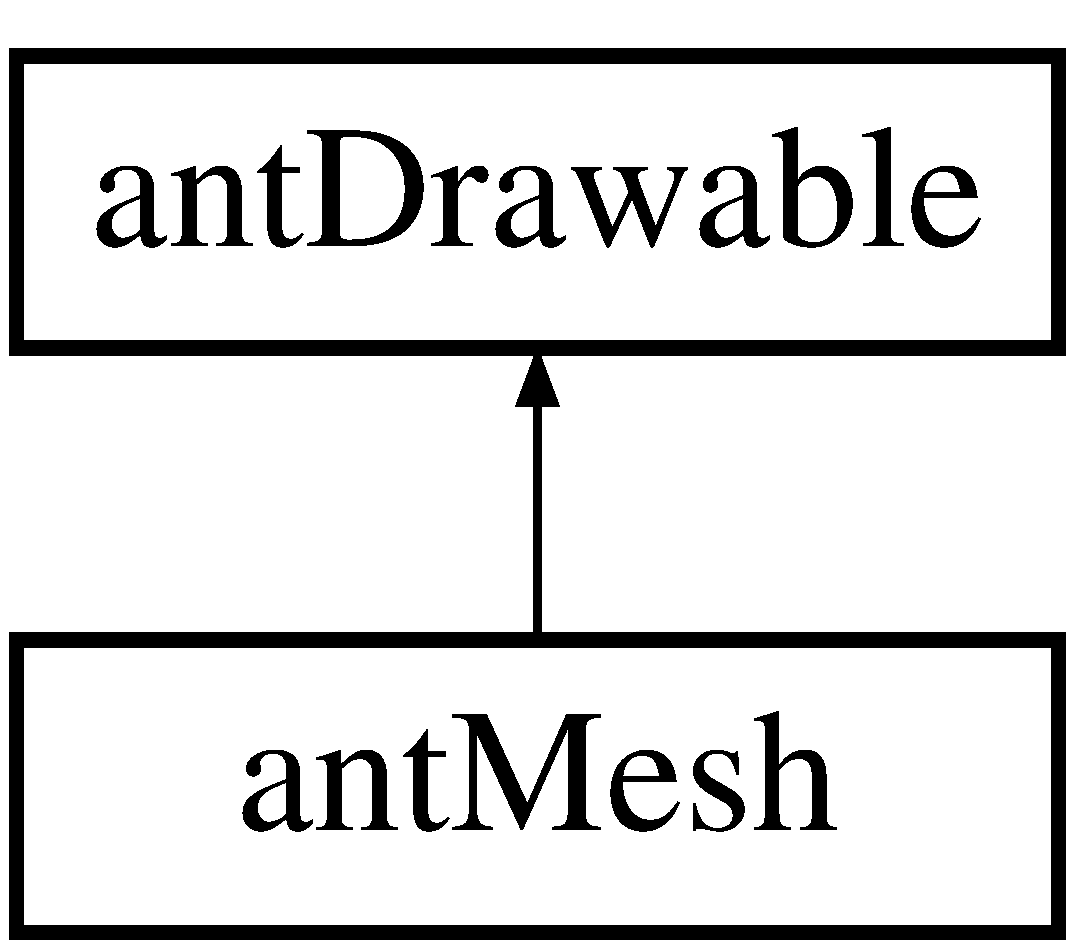
\includegraphics[height=2.000000cm]{classant_mesh}
\end{center}
\end{figure}
\subsection*{Public Member Functions}
\begin{DoxyCompactItemize}
\item 
\hypertarget{classant_mesh_a72ceed4cd84ffc04ab8775cbfb7bf171}{void {\bfseries fill} ()}\label{classant_mesh_a72ceed4cd84ffc04ab8775cbfb7bf171}

\end{DoxyCompactItemize}
\subsection*{Static Public Member Functions}
\begin{DoxyCompactItemize}
\item 
\hypertarget{classant_mesh_a7cefde0c04d7928c6394e1a10573d31b}{static ant\+Mesh\+Sh\+Ptr {\bfseries create\+From\+Obj\+File} (const std\+::string \&file\+\_\+path)}\label{classant_mesh_a7cefde0c04d7928c6394e1a10573d31b}

\end{DoxyCompactItemize}
\subsection*{Private Member Functions}
\begin{DoxyCompactItemize}
\item 
\hypertarget{classant_mesh_adb3128af13ce66a28abd285c01cacc3a}{{\bfseries ant\+Mesh} (int n\+Vertices)}\label{classant_mesh_adb3128af13ce66a28abd285c01cacc3a}

\end{DoxyCompactItemize}
\subsection*{Private Attributes}
\begin{DoxyCompactItemize}
\item 
\hypertarget{classant_mesh_aca39a8e65075996cb466d3378baf821b}{ant\+Mesh\+Wk\+Ptr {\bfseries m\+\_\+weak\+\_\+ptr}}\label{classant_mesh_aca39a8e65075996cb466d3378baf821b}

\end{DoxyCompactItemize}
\subsection*{Additional Inherited Members}


The documentation for this class was generated from the following file\+:\begin{DoxyCompactItemize}
\item 
/\+Users/anthonycouret/\+Developer/ant\+\_\+graphics/ant\+\_\+graphics/include/gl/ant\+Mesh.\+h\end{DoxyCompactItemize}

\hypertarget{classant_midi}{\section{ant\+Midi Class Reference}
\label{classant_midi}\index{ant\+Midi@{ant\+Midi}}
}
\subsection*{Public Member Functions}
\begin{DoxyCompactItemize}
\item 
\hypertarget{classant_midi_a971e0aeabc8cdf1920c5d61e7a0382c1}{bool {\bfseries get} (int $\ast$k\+\_\+byte, float $\ast$value\+\_\+byte)}\label{classant_midi_a971e0aeabc8cdf1920c5d61e7a0382c1}

\end{DoxyCompactItemize}
\subsection*{Static Public Member Functions}
\begin{DoxyCompactItemize}
\item 
\hypertarget{classant_midi_afbcec4b5057c75d7a9d672e4f8fffcda}{static ant\+Midi\+Sh\+Ptr {\bfseries create} ()}\label{classant_midi_afbcec4b5057c75d7a9d672e4f8fffcda}

\end{DoxyCompactItemize}
\subsection*{Static Private Member Functions}
\begin{DoxyCompactItemize}
\item 
\hypertarget{classant_midi_ae0f690b6cebaeed51f3559d72b5aa0d3}{static void {\bfseries finish} (int ignore)}\label{classant_midi_ae0f690b6cebaeed51f3559d72b5aa0d3}

\end{DoxyCompactItemize}
\subsection*{Private Attributes}
\begin{DoxyCompactItemize}
\item 
\hypertarget{classant_midi_ad89992ccbdf6d5d4a8be2a9f32ed71ab}{Rt\+Midi\+In $\ast$ {\bfseries m\+\_\+midi\+\_\+in}}\label{classant_midi_ad89992ccbdf6d5d4a8be2a9f32ed71ab}

\item 
\hypertarget{classant_midi_ae055bf54fa6007f3ae895d28bc020766}{ant\+Midi\+Wk\+Ptr {\bfseries m\+\_\+weak\+\_\+ptr}}\label{classant_midi_ae055bf54fa6007f3ae895d28bc020766}

\end{DoxyCompactItemize}
\subsection*{Static Private Attributes}
\begin{DoxyCompactItemize}
\item 
\hypertarget{classant_midi_a936ada34eb4af9b1437e72bcfcf098d7}{static bool {\bfseries m\+\_\+done}}\label{classant_midi_a936ada34eb4af9b1437e72bcfcf098d7}

\end{DoxyCompactItemize}


The documentation for this class was generated from the following file\+:\begin{DoxyCompactItemize}
\item 
/\+Users/anthonycouret/\+Developer/ant\+\_\+graphics/ant\+\_\+graphics/include/midi/ant\+Midi.\+h\end{DoxyCompactItemize}

\hypertarget{classant_obj_loader}{\section{ant\+Obj\+Loader Class Reference}
\label{classant_obj_loader}\index{ant\+Obj\+Loader@{ant\+Obj\+Loader}}
}
\subsection*{Public Member Functions}
\begin{DoxyCompactItemize}
\item 
\hypertarget{classant_obj_loader_a25c1b247ff0625e7927d8d4ad28a84c9}{bool {\bfseries has\+Vertices} ()}\label{classant_obj_loader_a25c1b247ff0625e7927d8d4ad28a84c9}

\item 
\hypertarget{classant_obj_loader_a97da01dcb9d2de37cb5866d801b6214f}{bool {\bfseries has\+Colors} ()}\label{classant_obj_loader_a97da01dcb9d2de37cb5866d801b6214f}

\item 
\hypertarget{classant_obj_loader_a882972daf1a8feaa45955263d919bd34}{bool {\bfseries has\+Tex\+Coords} ()}\label{classant_obj_loader_a882972daf1a8feaa45955263d919bd34}

\item 
\hypertarget{classant_obj_loader_a6cddb0d03795cdf6e00f4628f13f7b5e}{bool {\bfseries has\+Normals} ()}\label{classant_obj_loader_a6cddb0d03795cdf6e00f4628f13f7b5e}

\item 
\hypertarget{classant_obj_loader_a9601e51f1ba4cc475877ae6e8634832e}{bool {\bfseries load\+Vertices} (G\+Lfloat $\ast$vertices)}\label{classant_obj_loader_a9601e51f1ba4cc475877ae6e8634832e}

\item 
\hypertarget{classant_obj_loader_aaace717cd031e4c5f13c6120f30a3588}{bool {\bfseries load\+Colors} (G\+Lfloat $\ast$colors)}\label{classant_obj_loader_aaace717cd031e4c5f13c6120f30a3588}

\item 
\hypertarget{classant_obj_loader_a55146e7322d4a1e4b212466d8e2d096d}{bool {\bfseries load\+Normals} (G\+Lfloat $\ast$normals)}\label{classant_obj_loader_a55146e7322d4a1e4b212466d8e2d096d}

\item 
\hypertarget{classant_obj_loader_adb7978c3f4262e608d2a0475d4a57d96}{bool {\bfseries load\+Tex\+Coords} (G\+Lfloat $\ast$texcoords)}\label{classant_obj_loader_adb7978c3f4262e608d2a0475d4a57d96}

\item 
\hypertarget{classant_obj_loader_a00404bc86b3aa9aaef44ea0b3a4fda9b}{const int {\bfseries get\+N\+Vertices} ()}\label{classant_obj_loader_a00404bc86b3aa9aaef44ea0b3a4fda9b}

\end{DoxyCompactItemize}
\subsection*{Static Public Member Functions}
\begin{DoxyCompactItemize}
\item 
\hypertarget{classant_obj_loader_a92320806fcb86a263ba9b8d18bf981a3}{static ant\+Obj\+Loader\+Sh\+Ptr {\bfseries create} (const std\+::string \&file\+\_\+path)}\label{classant_obj_loader_a92320806fcb86a263ba9b8d18bf981a3}

\end{DoxyCompactItemize}
\subsection*{Private Member Functions}
\begin{DoxyCompactItemize}
\item 
\hypertarget{classant_obj_loader_a24d0e1dcd6069e7c13a822b1c42f980b}{{\bfseries ant\+Obj\+Loader} (const std\+::string \&file\+\_\+path)}\label{classant_obj_loader_a24d0e1dcd6069e7c13a822b1c42f980b}

\end{DoxyCompactItemize}
\subsection*{Private Attributes}
\begin{DoxyCompactItemize}
\item 
\hypertarget{classant_obj_loader_a346b1aff15e82516b09702a8eed63fa2}{bool {\bfseries m\+\_\+loaded}}\label{classant_obj_loader_a346b1aff15e82516b09702a8eed63fa2}

\item 
\hypertarget{classant_obj_loader_ab415218f6df9eb35bf15668f8d461644}{const ai\+Scene $\ast$ {\bfseries m\+\_\+scene}}\label{classant_obj_loader_ab415218f6df9eb35bf15668f8d461644}

\item 
\hypertarget{classant_obj_loader_ac98e373d38608b64a5bcce904b3e0451}{const ai\+Mesh $\ast$ {\bfseries m\+\_\+mesh}}\label{classant_obj_loader_ac98e373d38608b64a5bcce904b3e0451}

\item 
\hypertarget{classant_obj_loader_a57832a9c805c0efd9a307147ed00ae8c}{int {\bfseries m\+\_\+n\+Vertices}}\label{classant_obj_loader_a57832a9c805c0efd9a307147ed00ae8c}

\item 
\hypertarget{classant_obj_loader_aba3b7466d22a4b247e5635cdc27c49d8}{ant\+Obj\+Loader\+Wk\+Ptr {\bfseries m\+\_\+weak\+\_\+ptr}}\label{classant_obj_loader_aba3b7466d22a4b247e5635cdc27c49d8}

\end{DoxyCompactItemize}


The documentation for this class was generated from the following file\+:\begin{DoxyCompactItemize}
\item 
/\+Users/anthonycouret/\+Developer/ant\+Graphics/include/loader/ant\+Obj\+Loader.\+h\end{DoxyCompactItemize}

\hypertarget{classant_plane}{\section{ant\+Plane Class Reference}
\label{classant_plane}\index{ant\+Plane@{ant\+Plane}}
}
Inheritance diagram for ant\+Plane\+:\begin{figure}[H]
\begin{center}
\leavevmode
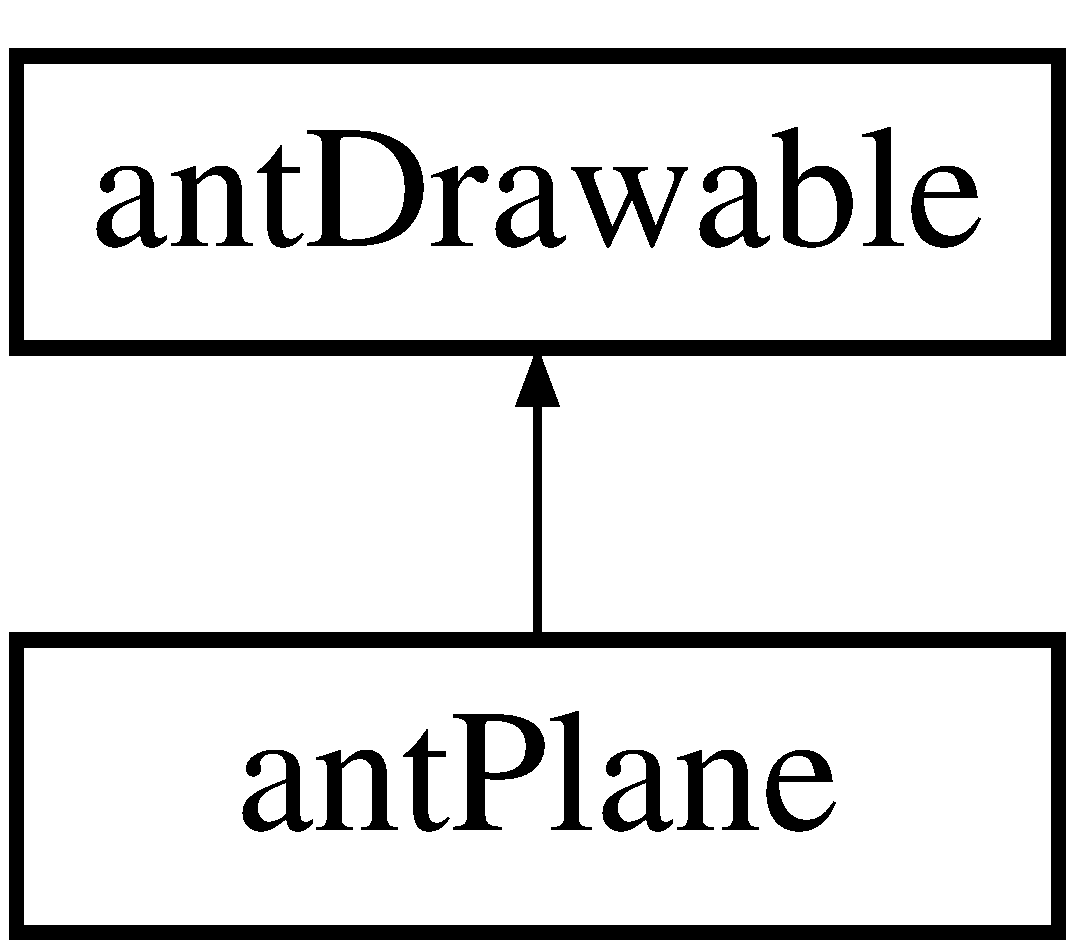
\includegraphics[height=2.000000cm]{classant_plane}
\end{center}
\end{figure}
\subsection*{Public Member Functions}
\begin{DoxyCompactItemize}
\item 
\hypertarget{classant_plane_ab159d806e8c8b6006c6d38532cb42957}{void {\bfseries generate\+Vertices} ()}\label{classant_plane_ab159d806e8c8b6006c6d38532cb42957}

\item 
\hypertarget{classant_plane_a0b1ff8ed4fc9bff018998ed735d70a76}{void {\bfseries generate\+Colors} (const ant\+R\+G\+B\+A \&color\+\_\+1, const ant\+R\+G\+B\+A \&color\+\_\+2)}\label{classant_plane_a0b1ff8ed4fc9bff018998ed735d70a76}

\item 
\hypertarget{classant_plane_a3cf33211145364ae415d7d197f835b4c}{void {\bfseries generate\+Normals} ()}\label{classant_plane_a3cf33211145364ae415d7d197f835b4c}

\item 
\hypertarget{classant_plane_a8bfac262c0c453354e6e9cfe5a3175e1}{void {\bfseries generate\+Tex\+Coords} ()}\label{classant_plane_a8bfac262c0c453354e6e9cfe5a3175e1}

\item 
\hypertarget{classant_plane_abb69c99d821189cf3a2b79d2738d7872}{virtual void {\bfseries draw} ()}\label{classant_plane_abb69c99d821189cf3a2b79d2738d7872}

\end{DoxyCompactItemize}
\subsection*{Static Public Member Functions}
\begin{DoxyCompactItemize}
\item 
\hypertarget{classant_plane_aa105beaf04d10d87a0049553eaf24619}{static ant\+Plane\+Sh\+Ptr {\bfseries create} (float width, float depth, int n\+Columns, int n\+Rows, int n\+Vbo=4, bool gen\+Colors=true, bool gen\+Normals=true, bool gen\+Tex\+Coords=true)}\label{classant_plane_aa105beaf04d10d87a0049553eaf24619}

\end{DoxyCompactItemize}
\subsection*{Private Member Functions}
\begin{DoxyCompactItemize}
\item 
\hypertarget{classant_plane_a247818056d0868caa48ae8fe8be7cea8}{{\bfseries ant\+Plane} (float width, float depth, int n\+Columns, int n\+Rows, int n\+Vbo, bool gen\+Colors, bool gen\+Normals, bool gen\+Tex\+Coords)}\label{classant_plane_a247818056d0868caa48ae8fe8be7cea8}

\end{DoxyCompactItemize}
\subsection*{Private Attributes}
\begin{DoxyCompactItemize}
\item 
\hypertarget{classant_plane_a149d1bb80ff074bad37bad7fd4aa6159}{float {\bfseries m\+\_\+width}}\label{classant_plane_a149d1bb80ff074bad37bad7fd4aa6159}

\item 
\hypertarget{classant_plane_a089bbfa1fbdada0c4fde3c95f8cc2177}{float {\bfseries m\+\_\+depth}}\label{classant_plane_a089bbfa1fbdada0c4fde3c95f8cc2177}

\item 
\hypertarget{classant_plane_aa6d27a983a39724bf78d282d32736a1e}{int {\bfseries m\+\_\+n\+Columns}}\label{classant_plane_aa6d27a983a39724bf78d282d32736a1e}

\item 
\hypertarget{classant_plane_a0d3ec74b12f96ee9c19def16de3f0d12}{int {\bfseries m\+\_\+n\+Rows}}\label{classant_plane_a0d3ec74b12f96ee9c19def16de3f0d12}

\item 
\hypertarget{classant_plane_a5026e9579dde0955193ad12bfd90f554}{ant\+Plane\+Wk\+Ptr {\bfseries m\+\_\+weak\+\_\+ptr}}\label{classant_plane_a5026e9579dde0955193ad12bfd90f554}

\end{DoxyCompactItemize}
\subsection*{Additional Inherited Members}


The documentation for this class was generated from the following file\+:\begin{DoxyCompactItemize}
\item 
/\+Users/anthonycouret/\+Developer/ant\+Graphics/include/primitives/ant\+Plane.\+h\end{DoxyCompactItemize}

\hypertarget{classant_point_light}{\section{ant\+Point\+Light Class Reference}
\label{classant_point_light}\index{ant\+Point\+Light@{ant\+Point\+Light}}
}
\subsection*{Public Member Functions}
\begin{DoxyCompactItemize}
\item 
\hypertarget{classant_point_light_a630a91019ee07f405b1afe7d2449bc53}{void {\bfseries set\+Position} (const ant\+Vec3 \&position)}\label{classant_point_light_a630a91019ee07f405b1afe7d2449bc53}

\item 
\hypertarget{classant_point_light_a8c51da56f08f230a417f2a867c3a0ff6}{void {\bfseries set\+Specular\+Color} (const ant\+R\+G\+B\+A \&color)}\label{classant_point_light_a8c51da56f08f230a417f2a867c3a0ff6}

\item 
\hypertarget{classant_point_light_ae1ed38562f6907d0d0a0923ca0388b4d}{ant\+Vec3 {\bfseries get\+Position} ()}\label{classant_point_light_ae1ed38562f6907d0d0a0923ca0388b4d}

\item 
\hypertarget{classant_point_light_abf843442d58947a608394a1438514c90}{ant\+R\+G\+B\+A {\bfseries get\+Specular\+Color} ()}\label{classant_point_light_abf843442d58947a608394a1438514c90}

\end{DoxyCompactItemize}
\subsection*{Static Public Member Functions}
\begin{DoxyCompactItemize}
\item 
\hypertarget{classant_point_light_a49c685f4d26ff6a6b5e2ae0452a3a695}{static ant\+Point\+Light\+Sh\+Ptr {\bfseries create} (const ant\+Vec3 \&position)}\label{classant_point_light_a49c685f4d26ff6a6b5e2ae0452a3a695}

\end{DoxyCompactItemize}
\subsection*{Protected Member Functions}
\begin{DoxyCompactItemize}
\item 
\hypertarget{classant_point_light_a7fdb42a6d2d32e34dc3a5404a2732c66}{{\bfseries ant\+Point\+Light} (const ant\+Vec3 \&position)}\label{classant_point_light_a7fdb42a6d2d32e34dc3a5404a2732c66}

\end{DoxyCompactItemize}
\subsection*{Protected Attributes}
\begin{DoxyCompactItemize}
\item 
\hypertarget{classant_point_light_adc09bb0f8f8435e2b7075bdde86f5ab6}{ant\+Vec3 {\bfseries m\+\_\+position}}\label{classant_point_light_adc09bb0f8f8435e2b7075bdde86f5ab6}

\item 
\hypertarget{classant_point_light_abdf53de5914cc5f50a0513e071ad7232}{ant\+R\+G\+B\+A {\bfseries m\+\_\+specular\+\_\+color}}\label{classant_point_light_abdf53de5914cc5f50a0513e071ad7232}

\item 
\hypertarget{classant_point_light_a1c001f73c63d0eac6b37829c626dee9a}{ant\+Point\+Light\+Wk\+Ptr {\bfseries m\+\_\+weak\+\_\+ptr}}\label{classant_point_light_a1c001f73c63d0eac6b37829c626dee9a}

\end{DoxyCompactItemize}


The documentation for this class was generated from the following file\+:\begin{DoxyCompactItemize}
\item 
/\+Users/anthonycouret/\+Developer/ant\+Graphics/include/light/ant\+Point\+Light.\+h\end{DoxyCompactItemize}

\hypertarget{classant_shader}{\section{ant\+Shader Class Reference}
\label{classant_shader}\index{ant\+Shader@{ant\+Shader}}
}
\subsection*{Static Public Member Functions}
\begin{DoxyCompactItemize}
\item 
static G\+Luint \hyperlink{classant_shader_a864581a4d2fe4e8591f9146c4c6afefd}{create\+Shader\+Program} (const std\+::string \&vertex\+\_\+shader, const std\+::string \&fragment\+\_\+shader)
\begin{DoxyCompactList}\small\item\em create a shader program \end{DoxyCompactList}\item 
\hypertarget{classant_shader_aa522313a8f85c99aa7e378e7539532f4}{static G\+Luint {\bfseries create\+Shader\+Program} (const std\+::string \&vertex\+\_\+shader, const std\+::string \&geometry\+\_\+shader, const std\+::string \&fragment\+\_\+shader)}\label{classant_shader_aa522313a8f85c99aa7e378e7539532f4}

\end{DoxyCompactItemize}
\subsection*{Static Private Member Functions}
\begin{DoxyCompactItemize}
\item 
\hypertarget{classant_shader_a0460ac64e8340914f89d2d273ba4bd76}{static G\+Lchar $\ast$ {\bfseries read\+File} (const std\+::string \&file\+\_\+path)}\label{classant_shader_a0460ac64e8340914f89d2d273ba4bd76}

\end{DoxyCompactItemize}


\subsection{Member Function Documentation}
\hypertarget{classant_shader_a864581a4d2fe4e8591f9146c4c6afefd}{\index{ant\+Shader@{ant\+Shader}!create\+Shader\+Program@{create\+Shader\+Program}}
\index{create\+Shader\+Program@{create\+Shader\+Program}!ant\+Shader@{ant\+Shader}}
\subsubsection[{create\+Shader\+Program}]{\setlength{\rightskip}{0pt plus 5cm}static G\+Luint ant\+Shader\+::create\+Shader\+Program (
\begin{DoxyParamCaption}
\item[{const std\+::string \&}]{vertex\+\_\+shader, }
\item[{const std\+::string \&}]{fragment\+\_\+shader}
\end{DoxyParamCaption}
)\hspace{0.3cm}{\ttfamily [static]}}}\label{classant_shader_a864581a4d2fe4e8591f9146c4c6afefd}


create a shader program 


\begin{DoxyParams}{Parameters}
{\em vertex\+\_\+shader} & vertex shader file path \\
\hline
{\em fragment\+\_\+shader} & fragment shader file path \\
\hline
\end{DoxyParams}
\begin{DoxyReturn}{Returns}
shader program id 
\end{DoxyReturn}


The documentation for this class was generated from the following file\+:\begin{DoxyCompactItemize}
\item 
/\+Users/anthonycouret/\+Developer/ant\+\_\+graphics/ant\+\_\+graphics/include/shader/ant\+Shader.\+h\end{DoxyCompactItemize}

\hypertarget{classant_skybox}{\section{ant\+Skybox Class Reference}
\label{classant_skybox}\index{ant\+Skybox@{ant\+Skybox}}
}
Inheritance diagram for ant\+Skybox\+:\begin{figure}[H]
\begin{center}
\leavevmode
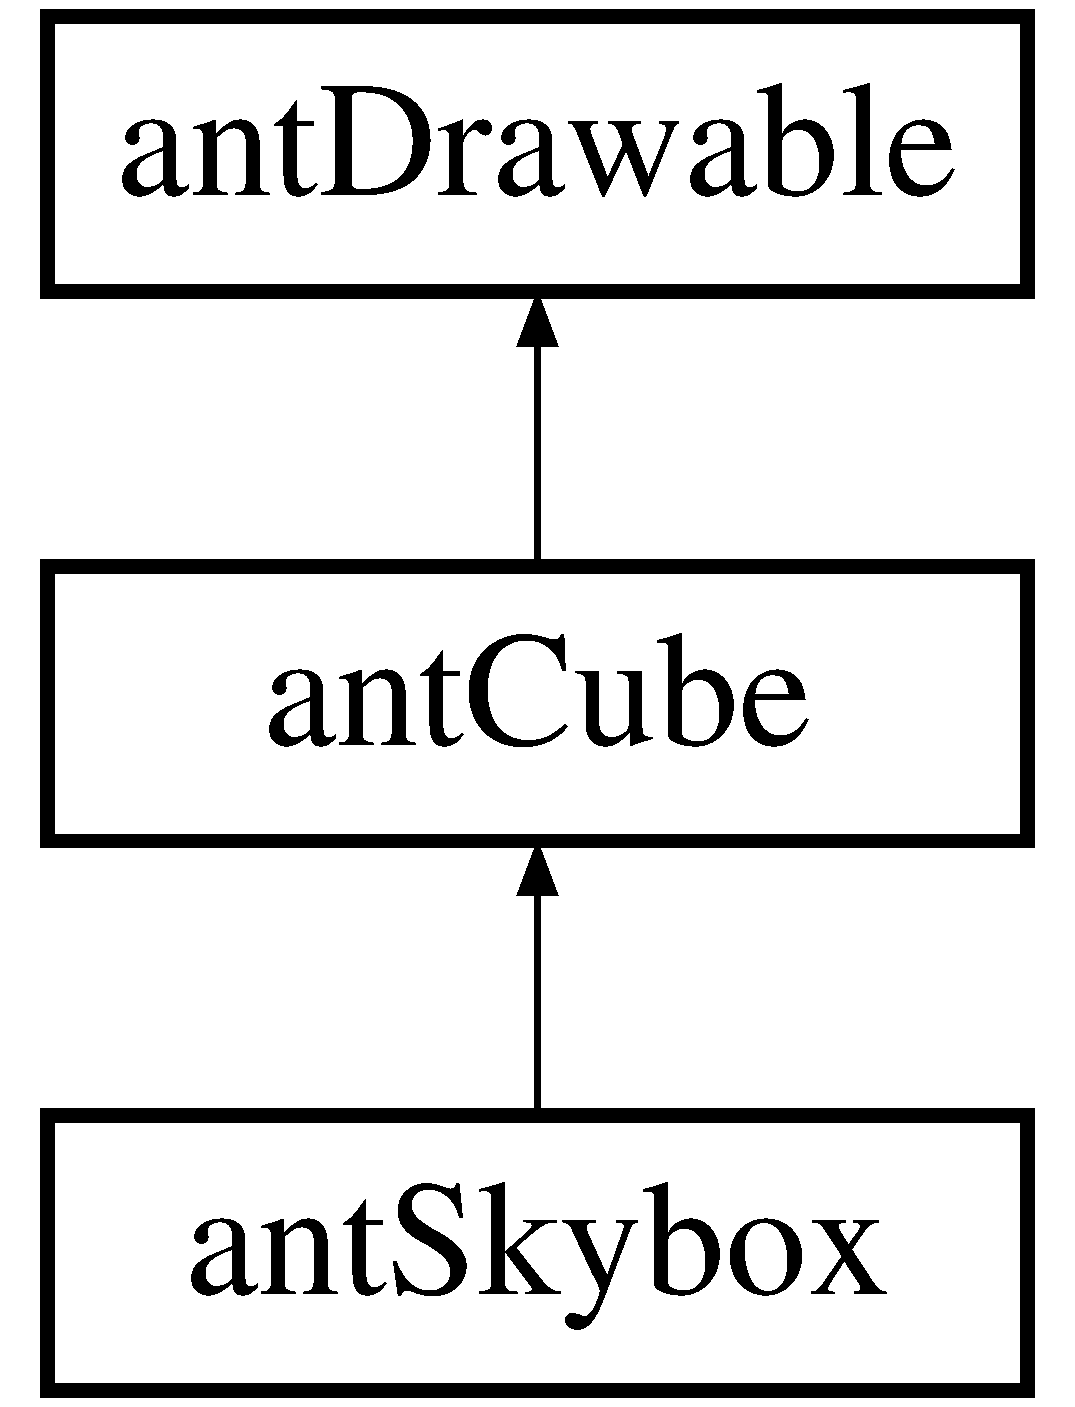
\includegraphics[height=3.000000cm]{classant_skybox}
\end{center}
\end{figure}
\subsection*{Public Member Functions}
\begin{DoxyCompactItemize}
\item 
\hypertarget{classant_skybox_a1832fdcc8a7dbed2da0c8a6b4b10dc6a}{G\+Luint {\bfseries get\+Textures} ()}\label{classant_skybox_a1832fdcc8a7dbed2da0c8a6b4b10dc6a}

\end{DoxyCompactItemize}
\subsection*{Static Public Member Functions}
\begin{DoxyCompactItemize}
\item 
\hypertarget{classant_skybox_a2e4c67b009ae90b0a3fd26b5784b8e9f}{static ant\+Skybox\+Sh\+Ptr {\bfseries create} (const std\+::string \&tex\+\_\+dir)}\label{classant_skybox_a2e4c67b009ae90b0a3fd26b5784b8e9f}

\end{DoxyCompactItemize}
\subsection*{Private Member Functions}
\begin{DoxyCompactItemize}
\item 
\hypertarget{classant_skybox_a0ae646ac446c4e320b5846ae02253787}{float {\bfseries map} (float v, float in\+\_\+min, float in\+\_\+max, float out\+\_\+min, float out\+\_\+max)}\label{classant_skybox_a0ae646ac446c4e320b5846ae02253787}

\item 
\hypertarget{classant_skybox_a2d09085e742ab68b22dcdc81fe8381d2}{ant\+Texture\+Sh\+Ptr {\bfseries get\+Face\+Texture} (int face)}\label{classant_skybox_a2d09085e742ab68b22dcdc81fe8381d2}

\item 
\hypertarget{classant_skybox_ad84025f713178b52e9575e00ededc0e4}{ant\+Texture\+Sh\+Ptr {\bfseries get\+Face\+Normal\+Tex} (int face)}\label{classant_skybox_ad84025f713178b52e9575e00ededc0e4}

\item 
\hypertarget{classant_skybox_a50dee4261170555d8ff75db2d8cea65d}{G\+Lenum {\bfseries get\+G\+L\+Cube\+Map\+Texture} (int face)}\label{classant_skybox_a50dee4261170555d8ff75db2d8cea65d}

\item 
\hypertarget{classant_skybox_ae03fee97951343ba8d41601efb64b978}{{\bfseries ant\+Skybox} (const std\+::string \&tex\+\_\+dir)}\label{classant_skybox_ae03fee97951343ba8d41601efb64b978}

\end{DoxyCompactItemize}
\subsection*{Private Attributes}
\begin{DoxyCompactItemize}
\item 
\hypertarget{classant_skybox_aa5de52bcffb36865301f2664a91b92e2}{G\+Luint {\bfseries m\+\_\+textures}}\label{classant_skybox_aa5de52bcffb36865301f2664a91b92e2}

\item 
\hypertarget{classant_skybox_abb6aaff3e119f947b40e712ef02f3464}{ant\+Texture\+Sh\+Ptr {\bfseries m\+\_\+front\+\_\+tex}}\label{classant_skybox_abb6aaff3e119f947b40e712ef02f3464}

\item 
\hypertarget{classant_skybox_a68c118d7fca016806ef2b0857f9a74bd}{ant\+Texture\+Sh\+Ptr {\bfseries m\+\_\+back\+\_\+tex}}\label{classant_skybox_a68c118d7fca016806ef2b0857f9a74bd}

\item 
\hypertarget{classant_skybox_a46c96fcd0162652bc8041480763da760}{ant\+Texture\+Sh\+Ptr {\bfseries m\+\_\+left\+\_\+tex}}\label{classant_skybox_a46c96fcd0162652bc8041480763da760}

\item 
\hypertarget{classant_skybox_a51fa3e38c692e62413a76bff3ac8b851}{ant\+Texture\+Sh\+Ptr {\bfseries m\+\_\+right\+\_\+tex}}\label{classant_skybox_a51fa3e38c692e62413a76bff3ac8b851}

\item 
\hypertarget{classant_skybox_ae1d8ca5af0ad395a0bda5ce7be5b9799}{ant\+Texture\+Sh\+Ptr {\bfseries m\+\_\+top\+\_\+tex}}\label{classant_skybox_ae1d8ca5af0ad395a0bda5ce7be5b9799}

\item 
\hypertarget{classant_skybox_ac3d6024649df82daaf7af8511c3e91fb}{ant\+Texture\+Sh\+Ptr {\bfseries m\+\_\+bottom\+\_\+tex}}\label{classant_skybox_ac3d6024649df82daaf7af8511c3e91fb}

\item 
\hypertarget{classant_skybox_a3acd43d844c506dbb955dc4911848725}{G\+Luint {\bfseries m\+\_\+tex\+\_\+normals}}\label{classant_skybox_a3acd43d844c506dbb955dc4911848725}

\item 
\hypertarget{classant_skybox_a0e3b50f2ca9bed6b0288e7ca4fe19c72}{ant\+Texture\+Sh\+Ptr {\bfseries m\+\_\+front\+\_\+norm}}\label{classant_skybox_a0e3b50f2ca9bed6b0288e7ca4fe19c72}

\item 
\hypertarget{classant_skybox_ab97c9db7a5daf60c779baf0a4830edc4}{ant\+Texture\+Sh\+Ptr {\bfseries m\+\_\+back\+\_\+norm}}\label{classant_skybox_ab97c9db7a5daf60c779baf0a4830edc4}

\item 
\hypertarget{classant_skybox_af8595eaa31f3499bf47b8774284d159a}{ant\+Texture\+Sh\+Ptr {\bfseries m\+\_\+left\+\_\+norm}}\label{classant_skybox_af8595eaa31f3499bf47b8774284d159a}

\item 
\hypertarget{classant_skybox_a98189f97cf4f29dc995cfc3cad81cc76}{ant\+Texture\+Sh\+Ptr {\bfseries m\+\_\+right\+\_\+norm}}\label{classant_skybox_a98189f97cf4f29dc995cfc3cad81cc76}

\item 
\hypertarget{classant_skybox_a19b09c73314d82158fafdc5f495ffb1c}{ant\+Texture\+Sh\+Ptr {\bfseries m\+\_\+top\+\_\+norm}}\label{classant_skybox_a19b09c73314d82158fafdc5f495ffb1c}

\item 
\hypertarget{classant_skybox_afe29da29d8b0b8c07771e5afc8116b08}{ant\+Texture\+Sh\+Ptr {\bfseries m\+\_\+bottom\+\_\+norm}}\label{classant_skybox_afe29da29d8b0b8c07771e5afc8116b08}

\item 
\hypertarget{classant_skybox_adafe8d00285291c51861c4309502a8a9}{ant\+Skybox\+Wk\+Ptr {\bfseries m\+\_\+weak\+\_\+ptr}}\label{classant_skybox_adafe8d00285291c51861c4309502a8a9}

\end{DoxyCompactItemize}
\subsection*{Additional Inherited Members}


The documentation for this class was generated from the following file\+:\begin{DoxyCompactItemize}
\item 
/\+Users/anthonycouret/\+Developer/ant\+\_\+graphics/ant\+\_\+graphics/include/environment/ant\+Skybox.\+h\end{DoxyCompactItemize}

\hypertarget{classant_sphere}{\section{ant\+Sphere Class Reference}
\label{classant_sphere}\index{ant\+Sphere@{ant\+Sphere}}
}
Inheritance diagram for ant\+Sphere\+:\begin{figure}[H]
\begin{center}
\leavevmode
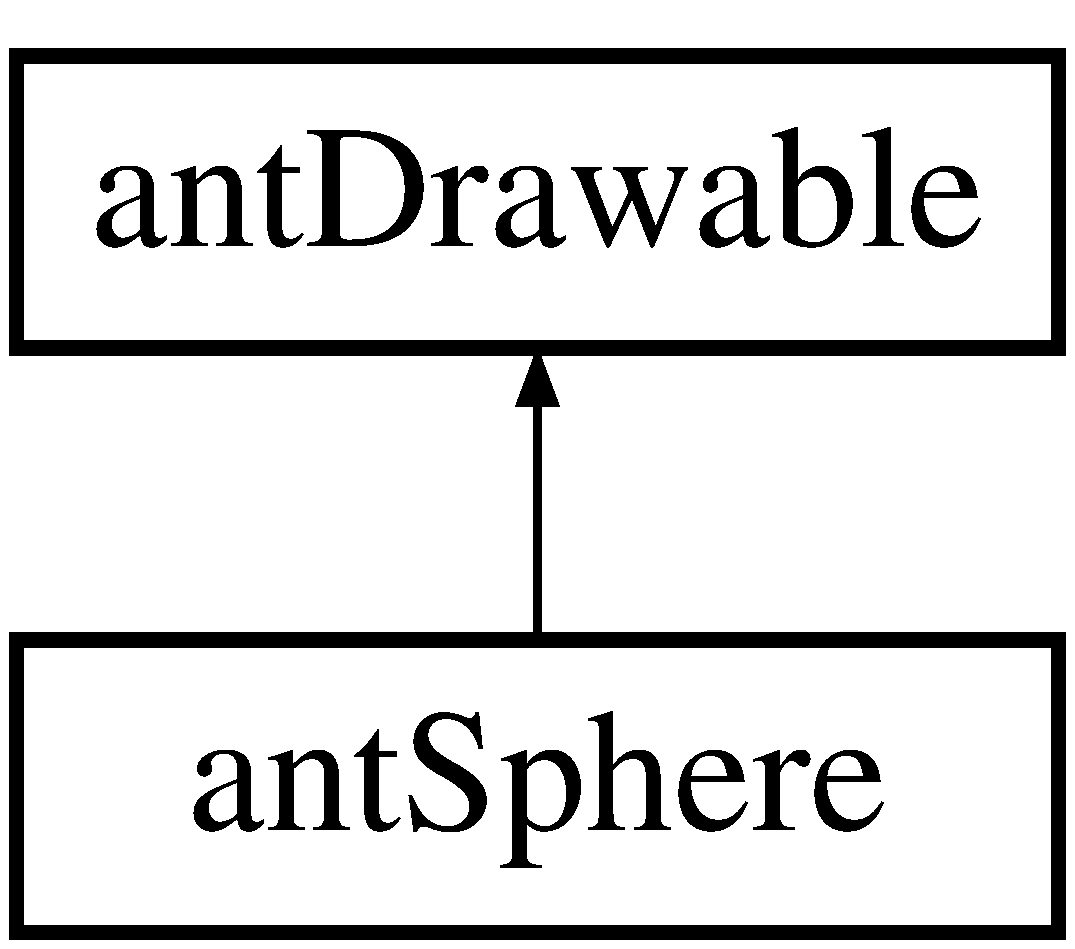
\includegraphics[height=2.000000cm]{classant_sphere}
\end{center}
\end{figure}
\subsection*{Static Public Member Functions}
\begin{DoxyCompactItemize}
\item 
\hypertarget{classant_sphere_a8bd56759dcdbd88c1ae05e00d426a527}{static ant\+Sphere\+Sh\+Ptr {\bfseries create} ()}\label{classant_sphere_a8bd56759dcdbd88c1ae05e00d426a527}

\end{DoxyCompactItemize}
\subsection*{Private Member Functions}
\begin{DoxyCompactItemize}
\item 
\hypertarget{classant_sphere_adb2cfd74c195ceb9c6c0a0274c170bc8}{void {\bfseries fill} ()}\label{classant_sphere_adb2cfd74c195ceb9c6c0a0274c170bc8}

\item 
\hypertarget{classant_sphere_a6dd3b41d2fe037bdb6b406abc29a28fc}{{\bfseries ant\+Sphere} (int n\+Vertices)}\label{classant_sphere_a6dd3b41d2fe037bdb6b406abc29a28fc}

\end{DoxyCompactItemize}
\subsection*{Private Attributes}
\begin{DoxyCompactItemize}
\item 
\hypertarget{classant_sphere_ad1891361ec747beaf4c333c8b5d9ec1f}{ant\+Sphere\+Wk\+Ptr {\bfseries m\+\_\+weak\+\_\+ptr}}\label{classant_sphere_ad1891361ec747beaf4c333c8b5d9ec1f}

\end{DoxyCompactItemize}
\subsection*{Additional Inherited Members}


The documentation for this class was generated from the following file\+:\begin{DoxyCompactItemize}
\item 
/\+Users/anthonycouret/\+Developer/ant\+Graphics/include/primitives/ant\+Sphere.\+h\end{DoxyCompactItemize}

\hypertarget{classant_texture}{\section{ant\+Texture Class Reference}
\label{classant_texture}\index{ant\+Texture@{ant\+Texture}}
}
\subsection*{Public Member Functions}
\begin{DoxyCompactItemize}
\item 
\hypertarget{classant_texture_a2dacc1d8b3e6eb518d113aa32ecabe25}{bool {\bfseries load\+Texture\+From\+File} (const std\+::string \&texture\+\_\+file)}\label{classant_texture_a2dacc1d8b3e6eb518d113aa32ecabe25}

\item 
\hypertarget{classant_texture_af9ba3984572f44a5fe427eacb97e24ea}{int {\bfseries get\+Width} ()}\label{classant_texture_af9ba3984572f44a5fe427eacb97e24ea}

\item 
\hypertarget{classant_texture_a2f551d638f9a1439160c809acc95264b}{int {\bfseries get\+Height} ()}\label{classant_texture_a2f551d638f9a1439160c809acc95264b}

\item 
\hypertarget{classant_texture_af222a9f8a0745455dfddd42c306746bb}{const unsigned char $\ast$ {\bfseries get\+Data} ()}\label{classant_texture_af222a9f8a0745455dfddd42c306746bb}

\end{DoxyCompactItemize}
\subsection*{Static Public Member Functions}
\begin{DoxyCompactItemize}
\item 
\hypertarget{classant_texture_a2bff013dfd61fa9717e0991c2d4b5450}{static ant\+Texture\+Sh\+Ptr {\bfseries create} ()}\label{classant_texture_a2bff013dfd61fa9717e0991c2d4b5450}

\end{DoxyCompactItemize}
\subsection*{Private Attributes}
\begin{DoxyCompactItemize}
\item 
\hypertarget{classant_texture_ade1b18b60443c11a750be1ff4c4e49b2}{int {\bfseries m\+\_\+width}}\label{classant_texture_ade1b18b60443c11a750be1ff4c4e49b2}

\item 
\hypertarget{classant_texture_a3a5886f800ff0cdf273a2eb3bdf93a15}{int {\bfseries m\+\_\+height}}\label{classant_texture_a3a5886f800ff0cdf273a2eb3bdf93a15}

\item 
\hypertarget{classant_texture_a6b48a2c81aa5739d0fe7494ac8924732}{int {\bfseries m\+\_\+n\+Channels}}\label{classant_texture_a6b48a2c81aa5739d0fe7494ac8924732}

\item 
\hypertarget{classant_texture_ac8aff5d0908959bf88a1c7860b7808df}{int {\bfseries m\+\_\+n\+Req\+Channels}}\label{classant_texture_ac8aff5d0908959bf88a1c7860b7808df}

\item 
\hypertarget{classant_texture_a797deb11ecf747457dbe5abcd54df7a0}{unsigned char $\ast$ {\bfseries m\+\_\+texture\+\_\+data}}\label{classant_texture_a797deb11ecf747457dbe5abcd54df7a0}

\item 
\hypertarget{classant_texture_a78aecdbf075ec87a470b905449b1cd9e}{ant\+Texture\+Wk\+Ptr {\bfseries m\+\_\+weak\+\_\+ptr}}\label{classant_texture_a78aecdbf075ec87a470b905449b1cd9e}

\end{DoxyCompactItemize}


The documentation for this class was generated from the following file\+:\begin{DoxyCompactItemize}
\item 
/\+Users/anthonycouret/\+Developer/ant\+Graphics/include/texture/ant\+Texture.\+h\end{DoxyCompactItemize}

\hypertarget{classant_vao}{\section{ant\+Vao Class Reference}
\label{classant_vao}\index{ant\+Vao@{ant\+Vao}}
}


vertex array object  




{\ttfamily \#include $<$ant\+Vao.\+h$>$}

\subsection*{Public Member Functions}
\begin{DoxyCompactItemize}
\item 
G\+Luint \hyperlink{classant_vao_a5efa0defead323c3c9b1190dc5189aa5}{get} (int index=0) const 
\item 
void \hyperlink{classant_vao_a92bfa6b08372260e2e14dd9ab184f02f}{bind} (int index)
\item 
void \hyperlink{classant_vao_a9cf8c3b9de6c6e0f279c4e8933f9b74e}{attrib} (G\+Luint location, G\+Lint attribs\+\_\+size, G\+Lenum type, G\+Lboolean normalized, G\+Lsizei stride, const G\+Lvoid $\ast$pointer)
\item 
\hypertarget{classant_vao_ac8b6f2233f83ba83271f006f3b0be189}{void {\bfseries enable} (G\+Luint location)}\label{classant_vao_ac8b6f2233f83ba83271f006f3b0be189}

\item 
\hypertarget{classant_vao_a7b0fea83df63c01718d7f8cbe1cdf261}{void {\bfseries disable} (G\+Luint location)}\label{classant_vao_a7b0fea83df63c01718d7f8cbe1cdf261}

\end{DoxyCompactItemize}
\subsection*{Static Public Member Functions}
\begin{DoxyCompactItemize}
\item 
static ant\+Vao\+Sh\+Ptr \hyperlink{classant_vao_a7a2663eecd76da3414e347541a0dd7c7}{create} (int n=1)
\end{DoxyCompactItemize}
\subsection*{Private Member Functions}
\begin{DoxyCompactItemize}
\item 
\hypertarget{classant_vao_aaf3959d8db304d527398936346f81567}{{\bfseries ant\+Vao} (int n)}\label{classant_vao_aaf3959d8db304d527398936346f81567}

\end{DoxyCompactItemize}
\subsection*{Private Attributes}
\begin{DoxyCompactItemize}
\item 
int \hyperlink{classant_vao_a18263ffbcdd4251a7789d5049023d8f8}{m\+\_\+n}
\item 
G\+Luint $\ast$ \hyperlink{classant_vao_a9ddb4ce72bd223c7da3b826eb7ab4e01}{m\+\_\+id}
\item 
\hypertarget{classant_vao_aa5e459e6ee6cfd1e49a58027d501c5d1}{ant\+Vao\+Wk\+Ptr {\bfseries m\+\_\+weak\+\_\+ptr}}\label{classant_vao_aa5e459e6ee6cfd1e49a58027d501c5d1}

\end{DoxyCompactItemize}


\subsection{Detailed Description}
vertex array object 

class \hyperlink{classant_vao}{ant\+Vao} 

\subsection{Member Function Documentation}
\hypertarget{classant_vao_a9cf8c3b9de6c6e0f279c4e8933f9b74e}{\index{ant\+Vao@{ant\+Vao}!attrib@{attrib}}
\index{attrib@{attrib}!ant\+Vao@{ant\+Vao}}
\subsubsection[{attrib}]{\setlength{\rightskip}{0pt plus 5cm}void ant\+Vao\+::attrib (
\begin{DoxyParamCaption}
\item[{G\+Luint}]{location, }
\item[{G\+Lint}]{attribs\+\_\+size, }
\item[{G\+Lenum}]{type, }
\item[{G\+Lboolean}]{normalized, }
\item[{G\+Lsizei}]{stride, }
\item[{const G\+Lvoid $\ast$}]{pointer}
\end{DoxyParamCaption}
)}}\label{classant_vao_a9cf8c3b9de6c6e0f279c4e8933f9b74e}
attrib


\begin{DoxyParams}{Parameters}
{\em index} & vao index \\
\hline
{\em size} & size ? !!! \\
\hline
\end{DoxyParams}
\hypertarget{classant_vao_a92bfa6b08372260e2e14dd9ab184f02f}{\index{ant\+Vao@{ant\+Vao}!bind@{bind}}
\index{bind@{bind}!ant\+Vao@{ant\+Vao}}
\subsubsection[{bind}]{\setlength{\rightskip}{0pt plus 5cm}void ant\+Vao\+::bind (
\begin{DoxyParamCaption}
\item[{int}]{index}
\end{DoxyParamCaption}
)}}\label{classant_vao_a92bfa6b08372260e2e14dd9ab184f02f}
bind


\begin{DoxyParams}{Parameters}
{\em index} & vao index \\
\hline
\end{DoxyParams}
\hypertarget{classant_vao_a7a2663eecd76da3414e347541a0dd7c7}{\index{ant\+Vao@{ant\+Vao}!create@{create}}
\index{create@{create}!ant\+Vao@{ant\+Vao}}
\subsubsection[{create}]{\setlength{\rightskip}{0pt plus 5cm}static ant\+Vao\+Sh\+Ptr ant\+Vao\+::create (
\begin{DoxyParamCaption}
\item[{int}]{n = {\ttfamily 1}}
\end{DoxyParamCaption}
)\hspace{0.3cm}{\ttfamily [static]}}}\label{classant_vao_a7a2663eecd76da3414e347541a0dd7c7}
static creation


\begin{DoxyParams}{Parameters}
{\em n} & number of vertex array objects \\
\hline
\end{DoxyParams}
\hypertarget{classant_vao_a5efa0defead323c3c9b1190dc5189aa5}{\index{ant\+Vao@{ant\+Vao}!get@{get}}
\index{get@{get}!ant\+Vao@{ant\+Vao}}
\subsubsection[{get}]{\setlength{\rightskip}{0pt plus 5cm}G\+Luint ant\+Vao\+::get (
\begin{DoxyParamCaption}
\item[{int}]{index = {\ttfamily 0}}
\end{DoxyParamCaption}
) const}}\label{classant_vao_a5efa0defead323c3c9b1190dc5189aa5}
get


\begin{DoxyParams}{Parameters}
{\em vao} & index \\
\hline
\end{DoxyParams}
\begin{DoxyReturn}{Returns}
vao id 
\end{DoxyReturn}


\subsection{Member Data Documentation}
\hypertarget{classant_vao_a9ddb4ce72bd223c7da3b826eb7ab4e01}{\index{ant\+Vao@{ant\+Vao}!m\+\_\+id@{m\+\_\+id}}
\index{m\+\_\+id@{m\+\_\+id}!ant\+Vao@{ant\+Vao}}
\subsubsection[{m\+\_\+id}]{\setlength{\rightskip}{0pt plus 5cm}G\+Luint$\ast$ ant\+Vao\+::m\+\_\+id\hspace{0.3cm}{\ttfamily [private]}}}\label{classant_vao_a9ddb4ce72bd223c7da3b826eb7ab4e01}
vertex array objects ids pointer \hypertarget{classant_vao_a18263ffbcdd4251a7789d5049023d8f8}{\index{ant\+Vao@{ant\+Vao}!m\+\_\+n@{m\+\_\+n}}
\index{m\+\_\+n@{m\+\_\+n}!ant\+Vao@{ant\+Vao}}
\subsubsection[{m\+\_\+n}]{\setlength{\rightskip}{0pt plus 5cm}int ant\+Vao\+::m\+\_\+n\hspace{0.3cm}{\ttfamily [private]}}}\label{classant_vao_a18263ffbcdd4251a7789d5049023d8f8}
number of vertex array objects 

The documentation for this class was generated from the following file\+:\begin{DoxyCompactItemize}
\item 
/\+Users/anthonycouret/\+Developer/ant\+\_\+graphics/ant\+\_\+graphics/include/gl/ant\+Vao.\+h\end{DoxyCompactItemize}

\hypertarget{classant_vbo}{\section{ant\+Vbo Class Reference}
\label{classant_vbo}\index{ant\+Vbo@{ant\+Vbo}}
}


vertex array object  




{\ttfamily \#include $<$ant\+Vbo.\+h$>$}

\subsection*{Public Member Functions}
\begin{DoxyCompactItemize}
\item 
\hyperlink{classant_vbo_abf307882f88ca5d1215c9e281e9e36de}{$\sim$ant\+Vbo} ()
\item 
G\+Luint \hyperlink{classant_vbo_afecdb59e8844479186c1d4f0753252df}{get} (int index=0) const 
\item 
void \hyperlink{classant_vbo_a6348372fe04cc909b526cc40166e1544}{bind} (int index)
\item 
void \hyperlink{classant_vbo_aef854ede5ec02a59bfa1bea378e36e49}{set\+Data} (G\+Lsizeiptr size, const G\+Lvoid $\ast$data, G\+Lenum usage)
\end{DoxyCompactItemize}
\subsection*{Static Public Member Functions}
\begin{DoxyCompactItemize}
\item 
static ant\+Vbo\+Sh\+Ptr \hyperlink{classant_vbo_a2bae5b06d160917e4db3761e738f8d96}{create} (int n=1, G\+Lenum target=G\+L\+\_\+\+A\+R\+R\+A\+Y\+\_\+\+B\+U\+F\+F\+E\+R)
\end{DoxyCompactItemize}
\subsection*{Private Member Functions}
\begin{DoxyCompactItemize}
\item 
\hypertarget{classant_vbo_a18c59e211890a63677ab263ee8cf2888}{{\bfseries ant\+Vbo} (int n, G\+Lenum target)}\label{classant_vbo_a18c59e211890a63677ab263ee8cf2888}

\end{DoxyCompactItemize}
\subsection*{Private Attributes}
\begin{DoxyCompactItemize}
\item 
int \hyperlink{classant_vbo_aa470c365da54128248ff3cf82a13bb1d}{m\+\_\+n}
\item 
G\+Luint $\ast$ \hyperlink{classant_vbo_ad9d6ae592ea4f03caf48fd98ce5660c0}{m\+\_\+id}
\item 
\hypertarget{classant_vbo_a9f22d5a5783c19697a7d0d4a78bfe1f0}{G\+Lenum {\bfseries m\+\_\+target}}\label{classant_vbo_a9f22d5a5783c19697a7d0d4a78bfe1f0}

\item 
\hypertarget{classant_vbo_a76be179a1c3212b5e88bdbc84aafd222}{ant\+Vbo\+Wk\+Ptr {\bfseries m\+\_\+weak\+\_\+ptr}}\label{classant_vbo_a76be179a1c3212b5e88bdbc84aafd222}

\end{DoxyCompactItemize}


\subsection{Detailed Description}
vertex array object 

class \hyperlink{classant_vao}{ant\+Vao} 

\subsection{Constructor \& Destructor Documentation}
\hypertarget{classant_vbo_abf307882f88ca5d1215c9e281e9e36de}{\index{ant\+Vbo@{ant\+Vbo}!````~ant\+Vbo@{$\sim$ant\+Vbo}}
\index{````~ant\+Vbo@{$\sim$ant\+Vbo}!ant\+Vbo@{ant\+Vbo}}
\subsubsection[{$\sim$ant\+Vbo}]{\setlength{\rightskip}{0pt plus 5cm}ant\+Vbo\+::$\sim$ant\+Vbo (
\begin{DoxyParamCaption}
{}
\end{DoxyParamCaption}
)}}\label{classant_vbo_abf307882f88ca5d1215c9e281e9e36de}
destructor 

\subsection{Member Function Documentation}
\hypertarget{classant_vbo_a6348372fe04cc909b526cc40166e1544}{\index{ant\+Vbo@{ant\+Vbo}!bind@{bind}}
\index{bind@{bind}!ant\+Vbo@{ant\+Vbo}}
\subsubsection[{bind}]{\setlength{\rightskip}{0pt plus 5cm}void ant\+Vbo\+::bind (
\begin{DoxyParamCaption}
\item[{int}]{index}
\end{DoxyParamCaption}
)}}\label{classant_vbo_a6348372fe04cc909b526cc40166e1544}
bind


\begin{DoxyParams}{Parameters}
{\em index} & vbo index \\
\hline
\end{DoxyParams}
\hypertarget{classant_vbo_a2bae5b06d160917e4db3761e738f8d96}{\index{ant\+Vbo@{ant\+Vbo}!create@{create}}
\index{create@{create}!ant\+Vbo@{ant\+Vbo}}
\subsubsection[{create}]{\setlength{\rightskip}{0pt plus 5cm}static ant\+Vbo\+Sh\+Ptr ant\+Vbo\+::create (
\begin{DoxyParamCaption}
\item[{int}]{n = {\ttfamily 1}, }
\item[{G\+Lenum}]{target = {\ttfamily GL\+\_\+ARRAY\+\_\+BUFFER}}
\end{DoxyParamCaption}
)\hspace{0.3cm}{\ttfamily [static]}}}\label{classant_vbo_a2bae5b06d160917e4db3761e738f8d96}
static creation


\begin{DoxyParams}{Parameters}
{\em n} & number of vertex buffer objects \\
\hline
\end{DoxyParams}
\hypertarget{classant_vbo_afecdb59e8844479186c1d4f0753252df}{\index{ant\+Vbo@{ant\+Vbo}!get@{get}}
\index{get@{get}!ant\+Vbo@{ant\+Vbo}}
\subsubsection[{get}]{\setlength{\rightskip}{0pt plus 5cm}G\+Luint ant\+Vbo\+::get (
\begin{DoxyParamCaption}
\item[{int}]{index = {\ttfamily 0}}
\end{DoxyParamCaption}
) const}}\label{classant_vbo_afecdb59e8844479186c1d4f0753252df}
get


\begin{DoxyParams}{Parameters}
{\em index} & vbo index \\
\hline
\end{DoxyParams}
\begin{DoxyReturn}{Returns}
vbo id 
\end{DoxyReturn}
\hypertarget{classant_vbo_aef854ede5ec02a59bfa1bea378e36e49}{\index{ant\+Vbo@{ant\+Vbo}!set\+Data@{set\+Data}}
\index{set\+Data@{set\+Data}!ant\+Vbo@{ant\+Vbo}}
\subsubsection[{set\+Data}]{\setlength{\rightskip}{0pt plus 5cm}void ant\+Vbo\+::set\+Data (
\begin{DoxyParamCaption}
\item[{G\+Lsizeiptr}]{size, }
\item[{const G\+Lvoid $\ast$}]{data, }
\item[{G\+Lenum}]{usage}
\end{DoxyParamCaption}
)}}\label{classant_vbo_aef854ede5ec02a59bfa1bea378e36e49}
set\+Data


\begin{DoxyParams}{Parameters}
{\em size} & buffer size \\
\hline
{\em data} & data pointer \\
\hline
\end{DoxyParams}


\subsection{Member Data Documentation}
\hypertarget{classant_vbo_ad9d6ae592ea4f03caf48fd98ce5660c0}{\index{ant\+Vbo@{ant\+Vbo}!m\+\_\+id@{m\+\_\+id}}
\index{m\+\_\+id@{m\+\_\+id}!ant\+Vbo@{ant\+Vbo}}
\subsubsection[{m\+\_\+id}]{\setlength{\rightskip}{0pt plus 5cm}G\+Luint$\ast$ ant\+Vbo\+::m\+\_\+id\hspace{0.3cm}{\ttfamily [private]}}}\label{classant_vbo_ad9d6ae592ea4f03caf48fd98ce5660c0}
vertex buffer objects ids pointer \hypertarget{classant_vbo_aa470c365da54128248ff3cf82a13bb1d}{\index{ant\+Vbo@{ant\+Vbo}!m\+\_\+n@{m\+\_\+n}}
\index{m\+\_\+n@{m\+\_\+n}!ant\+Vbo@{ant\+Vbo}}
\subsubsection[{m\+\_\+n}]{\setlength{\rightskip}{0pt plus 5cm}int ant\+Vbo\+::m\+\_\+n\hspace{0.3cm}{\ttfamily [private]}}}\label{classant_vbo_aa470c365da54128248ff3cf82a13bb1d}
number of vertex buffer objects 

The documentation for this class was generated from the following file\+:\begin{DoxyCompactItemize}
\item 
/\+Users/anthonycouret/\+Developer/ant\+\_\+graphics/ant\+\_\+graphics/include/gl/ant\+Vbo.\+h\end{DoxyCompactItemize}

\hypertarget{classant_window}{\section{ant\+Window Class Reference}
\label{classant_window}\index{ant\+Window@{ant\+Window}}
}


to define a glfw window with an opengl context  




{\ttfamily \#include $<$ant\+Window.\+h$>$}

\subsection*{Public Member Functions}
\begin{DoxyCompactItemize}
\item 
G\+L\+F\+Wwindow $\ast$ \hyperlink{classant_window_ae28c1d4b125dd3f63fe341bf1d62e844}{get\+Window} ()
\begin{DoxyCompactList}\small\item\em render the \hyperlink{classant_window}{ant\+Window} object \end{DoxyCompactList}\item 
\hypertarget{classant_window_a42d7686bd139117a7ec1211e9e983684}{int {\bfseries get\+Width} () const }\label{classant_window_a42d7686bd139117a7ec1211e9e983684}

\item 
\hypertarget{classant_window_a8b82e64b718ce3f18ab1745e6dec9e95}{int {\bfseries get\+Height} () const }\label{classant_window_a8b82e64b718ce3f18ab1745e6dec9e95}

\item 
void \hyperlink{classant_window_a8546d18d1de59e9320b186d2162237e9}{update\+F\+P\+S\+Counter} (void)
\begin{DoxyCompactList}\small\item\em update the frames per second counter \end{DoxyCompactList}\item 
\hypertarget{classant_window_aca207a01f3103ea9edf6907ccd7311c9}{void {\bfseries swap\+And\+Poll} (void)}\label{classant_window_aca207a01f3103ea9edf6907ccd7311c9}

\item 
\hypertarget{classant_window_ad94c5ab65a013247cd59fa109e4d8805}{void {\bfseries update\+Key\+Mouse} (double $\ast$m\+\_\+mouse\+\_\+x\+\_\+pos, double $\ast$m\+\_\+mouse\+\_\+y\+\_\+pos)}\label{classant_window_ad94c5ab65a013247cd59fa109e4d8805}

\item 
\hypertarget{classant_window_acde1aace224a84c9c51d858932cd3e9d}{void {\bfseries viewport} ()}\label{classant_window_acde1aace224a84c9c51d858932cd3e9d}

\item 
void \hyperlink{classant_window_a6e12ebc5212196d5eae855762d182782}{print\+Window\+Status} (void)
\begin{DoxyCompactList}\small\item\em stream out informations about the \hyperlink{classant_window}{ant\+Window} object \end{DoxyCompactList}\item 
\hyperlink{classant_window_a1d59042b3c9a5e98db451ce13b0d0553}{$\sim$ant\+Window} ()
\begin{DoxyCompactList}\small\item\em destructor \end{DoxyCompactList}\end{DoxyCompactItemize}
\subsection*{Static Public Member Functions}
\begin{DoxyCompactItemize}
\item 
static ant\+Window\+Sh\+Ptr \hyperlink{classant_window_ad91cfd2dcb6c03472036ab5c2336b239}{create} (int width, int height, const std\+::string \&title)
\begin{DoxyCompactList}\small\item\em static method to create an \hyperlink{classant_window}{ant\+Window} object \end{DoxyCompactList}\end{DoxyCompactItemize}
\subsection*{Private Member Functions}
\begin{DoxyCompactItemize}
\item 
\hyperlink{classant_window_a8587e92cdc039ad0d3e5dbddd6b37600}{ant\+Window} (int width, int height, const std\+::string \&title)
\begin{DoxyCompactList}\small\item\em constructor \end{DoxyCompactList}\item 
\hypertarget{classant_window_ad85470c2398926767305d423404ad4db}{void {\bfseries init} ()}\label{classant_window_ad85470c2398926767305d423404ad4db}

\end{DoxyCompactItemize}
\subsection*{Private Attributes}
\begin{DoxyCompactItemize}
\item 
ant\+Window\+Wk\+Ptr \hyperlink{classant_window_a44da6525e4278681d0563347ca970bbc}{m\+\_\+weak\+\_\+ptr}
\item 
G\+L\+F\+Wwindow $\ast$ \hyperlink{classant_window_a8b77985c8b4772027e1cbed42ce67daf}{m\+\_\+window\+\_\+ptr}
\item 
std\+::string \hyperlink{classant_window_a6799e6207a4367630aa5a7a0603bafbb}{m\+\_\+title}
\item 
int \hyperlink{classant_window_ae50857682369f77c9fab71c64d3d8299}{m\+\_\+width}
\item 
int \hyperlink{classant_window_a81b5d1fc4f545fbf76fa63d0292494b8}{m\+\_\+height}
\end{DoxyCompactItemize}


\subsection{Detailed Description}
to define a glfw window with an opengl context 

class \hyperlink{classant_window}{ant\+Window} 

\subsection{Constructor \& Destructor Documentation}
\hypertarget{classant_window_a1d59042b3c9a5e98db451ce13b0d0553}{\index{ant\+Window@{ant\+Window}!````~ant\+Window@{$\sim$ant\+Window}}
\index{````~ant\+Window@{$\sim$ant\+Window}!ant\+Window@{ant\+Window}}
\subsubsection[{$\sim$ant\+Window}]{\setlength{\rightskip}{0pt plus 5cm}ant\+Window\+::$\sim$ant\+Window (
\begin{DoxyParamCaption}
{}
\end{DoxyParamCaption}
)}}\label{classant_window_a1d59042b3c9a5e98db451ce13b0d0553}


destructor 

$\sim$ant\+Wndow \hypertarget{classant_window_a8587e92cdc039ad0d3e5dbddd6b37600}{\index{ant\+Window@{ant\+Window}!ant\+Window@{ant\+Window}}
\index{ant\+Window@{ant\+Window}!ant\+Window@{ant\+Window}}
\subsubsection[{ant\+Window}]{\setlength{\rightskip}{0pt plus 5cm}ant\+Window\+::ant\+Window (
\begin{DoxyParamCaption}
\item[{int}]{width, }
\item[{int}]{height, }
\item[{const std\+::string \&}]{title}
\end{DoxyParamCaption}
)\hspace{0.3cm}{\ttfamily [private]}}}\label{classant_window_a8587e92cdc039ad0d3e5dbddd6b37600}


constructor 

\hyperlink{classant_window}{ant\+Window} 
\begin{DoxyParams}{Parameters}
{\em width} & window width \\
\hline
{\em height} & window height \\
\hline
{\em title} & window title \\
\hline
{\em app\+\_\+sptr} & \hyperlink{classant_abstract_app}{ant\+Abstract\+App} implementation shared pointer \\
\hline
\end{DoxyParams}


\subsection{Member Function Documentation}
\hypertarget{classant_window_ad91cfd2dcb6c03472036ab5c2336b239}{\index{ant\+Window@{ant\+Window}!create@{create}}
\index{create@{create}!ant\+Window@{ant\+Window}}
\subsubsection[{create}]{\setlength{\rightskip}{0pt plus 5cm}static ant\+Window\+Sh\+Ptr ant\+Window\+::create (
\begin{DoxyParamCaption}
\item[{int}]{width, }
\item[{int}]{height, }
\item[{const std\+::string \&}]{title}
\end{DoxyParamCaption}
)\hspace{0.3cm}{\ttfamily [static]}}}\label{classant_window_ad91cfd2dcb6c03472036ab5c2336b239}


static method to create an \hyperlink{classant_window}{ant\+Window} object 

create 
\begin{DoxyParams}{Parameters}
{\em width} & window width \\
\hline
{\em height} & window height \\
\hline
{\em title} & window title \\
\hline
{\em app\+\_\+sptr} & \hyperlink{classant_abstract_app}{ant\+Abstract\+App} implementation shared pointer\\
\hline
\end{DoxyParams}
\begin{DoxyReturn}{Returns}
an \hyperlink{classant_window}{ant\+Window} shared pointer 
\end{DoxyReturn}
\hypertarget{classant_window_ae28c1d4b125dd3f63fe341bf1d62e844}{\index{ant\+Window@{ant\+Window}!get\+Window@{get\+Window}}
\index{get\+Window@{get\+Window}!ant\+Window@{ant\+Window}}
\subsubsection[{get\+Window}]{\setlength{\rightskip}{0pt plus 5cm}G\+L\+F\+Wwindow$\ast$ ant\+Window\+::get\+Window (
\begin{DoxyParamCaption}
{}
\end{DoxyParamCaption}
)}}\label{classant_window_ae28c1d4b125dd3f63fe341bf1d62e844}


render the \hyperlink{classant_window}{ant\+Window} object 

render \hypertarget{classant_window_a6e12ebc5212196d5eae855762d182782}{\index{ant\+Window@{ant\+Window}!print\+Window\+Status@{print\+Window\+Status}}
\index{print\+Window\+Status@{print\+Window\+Status}!ant\+Window@{ant\+Window}}
\subsubsection[{print\+Window\+Status}]{\setlength{\rightskip}{0pt plus 5cm}void ant\+Window\+::print\+Window\+Status (
\begin{DoxyParamCaption}
\item[{void}]{}
\end{DoxyParamCaption}
)}}\label{classant_window_a6e12ebc5212196d5eae855762d182782}


stream out informations about the \hyperlink{classant_window}{ant\+Window} object 

print\+Wiwdow\+Status \hypertarget{classant_window_a8546d18d1de59e9320b186d2162237e9}{\index{ant\+Window@{ant\+Window}!update\+F\+P\+S\+Counter@{update\+F\+P\+S\+Counter}}
\index{update\+F\+P\+S\+Counter@{update\+F\+P\+S\+Counter}!ant\+Window@{ant\+Window}}
\subsubsection[{update\+F\+P\+S\+Counter}]{\setlength{\rightskip}{0pt plus 5cm}void ant\+Window\+::update\+F\+P\+S\+Counter (
\begin{DoxyParamCaption}
\item[{void}]{}
\end{DoxyParamCaption}
)}}\label{classant_window_a8546d18d1de59e9320b186d2162237e9}


update the frames per second counter 

update\+F\+P\+S\+C\+Ounter 
\begin{DoxyParams}{Parameters}
{\em window\+\_\+ptr} & a \\
\hline
\end{DoxyParams}


\subsection{Member Data Documentation}
\hypertarget{classant_window_a81b5d1fc4f545fbf76fa63d0292494b8}{\index{ant\+Window@{ant\+Window}!m\+\_\+height@{m\+\_\+height}}
\index{m\+\_\+height@{m\+\_\+height}!ant\+Window@{ant\+Window}}
\subsubsection[{m\+\_\+height}]{\setlength{\rightskip}{0pt plus 5cm}int ant\+Window\+::m\+\_\+height\hspace{0.3cm}{\ttfamily [private]}}}\label{classant_window_a81b5d1fc4f545fbf76fa63d0292494b8}
window height \hypertarget{classant_window_a6799e6207a4367630aa5a7a0603bafbb}{\index{ant\+Window@{ant\+Window}!m\+\_\+title@{m\+\_\+title}}
\index{m\+\_\+title@{m\+\_\+title}!ant\+Window@{ant\+Window}}
\subsubsection[{m\+\_\+title}]{\setlength{\rightskip}{0pt plus 5cm}std\+::string ant\+Window\+::m\+\_\+title\hspace{0.3cm}{\ttfamily [private]}}}\label{classant_window_a6799e6207a4367630aa5a7a0603bafbb}
window title \hypertarget{classant_window_a44da6525e4278681d0563347ca970bbc}{\index{ant\+Window@{ant\+Window}!m\+\_\+weak\+\_\+ptr@{m\+\_\+weak\+\_\+ptr}}
\index{m\+\_\+weak\+\_\+ptr@{m\+\_\+weak\+\_\+ptr}!ant\+Window@{ant\+Window}}
\subsubsection[{m\+\_\+weak\+\_\+ptr}]{\setlength{\rightskip}{0pt plus 5cm}ant\+Window\+Wk\+Ptr ant\+Window\+::m\+\_\+weak\+\_\+ptr\hspace{0.3cm}{\ttfamily [private]}}}\label{classant_window_a44da6525e4278681d0563347ca970bbc}
weak pointer \hypertarget{classant_window_ae50857682369f77c9fab71c64d3d8299}{\index{ant\+Window@{ant\+Window}!m\+\_\+width@{m\+\_\+width}}
\index{m\+\_\+width@{m\+\_\+width}!ant\+Window@{ant\+Window}}
\subsubsection[{m\+\_\+width}]{\setlength{\rightskip}{0pt plus 5cm}int ant\+Window\+::m\+\_\+width\hspace{0.3cm}{\ttfamily [private]}}}\label{classant_window_ae50857682369f77c9fab71c64d3d8299}
window width \hypertarget{classant_window_a8b77985c8b4772027e1cbed42ce67daf}{\index{ant\+Window@{ant\+Window}!m\+\_\+window\+\_\+ptr@{m\+\_\+window\+\_\+ptr}}
\index{m\+\_\+window\+\_\+ptr@{m\+\_\+window\+\_\+ptr}!ant\+Window@{ant\+Window}}
\subsubsection[{m\+\_\+window\+\_\+ptr}]{\setlength{\rightskip}{0pt plus 5cm}G\+L\+F\+Wwindow$\ast$ ant\+Window\+::m\+\_\+window\+\_\+ptr\hspace{0.3cm}{\ttfamily [private]}}}\label{classant_window_a8b77985c8b4772027e1cbed42ce67daf}
glfw window pointer 

The documentation for this class was generated from the following file\+:\begin{DoxyCompactItemize}
\item 
/\+Users/anthonycouret/\+Developer/ant\+\_\+graphics/ant\+\_\+graphics/include/window/ant\+Window.\+h\end{DoxyCompactItemize}

\hypertarget{structmat3}{\section{mat3 Struct Reference}
\label{structmat3}\index{mat3@{mat3}}
}
\subsection*{Public Member Functions}
\begin{DoxyCompactItemize}
\item 
\hypertarget{structmat3_ad5f393d1a6f7986207680e54e81f9906}{{\bfseries mat3} (float a, float b, float c, float d, float e, float f, float g, float h, float i)}\label{structmat3_ad5f393d1a6f7986207680e54e81f9906}

\end{DoxyCompactItemize}
\subsection*{Public Attributes}
\begin{DoxyCompactItemize}
\item 
\hypertarget{structmat3_af5c67cec8668816c844bfd3f097f9eb2}{float {\bfseries m} \mbox{[}9\mbox{]}}\label{structmat3_af5c67cec8668816c844bfd3f097f9eb2}

\end{DoxyCompactItemize}


The documentation for this struct was generated from the following file\+:\begin{DoxyCompactItemize}
\item 
/\+Users/anthonycouret/\+Developer/ant\+Graphics/include/math/maths\+\_\+funcs.\+h\end{DoxyCompactItemize}

\hypertarget{structmat4}{\section{mat4 Struct Reference}
\label{structmat4}\index{mat4@{mat4}}
}
\subsection*{Public Member Functions}
\begin{DoxyCompactItemize}
\item 
\hypertarget{structmat4_aa23388c850e1826e266a640d914e6119}{{\bfseries mat4} (float a, float b, float c, float d, float e, float f, float g, float h, float i, float j, float k, float l, float mm, float n, float o, float p)}\label{structmat4_aa23388c850e1826e266a640d914e6119}

\item 
\hypertarget{structmat4_ad9b252b1e4b560445d77f839bb420348}{\hyperlink{structvec4}{vec4} {\bfseries operator$\ast$} (const \hyperlink{structvec4}{vec4} \&rhs)}\label{structmat4_ad9b252b1e4b560445d77f839bb420348}

\item 
\hypertarget{structmat4_a0714c730bc200119265535b40b980ee4}{\hyperlink{structmat4}{mat4} {\bfseries operator$\ast$} (const \hyperlink{structmat4}{mat4} \&rhs)}\label{structmat4_a0714c730bc200119265535b40b980ee4}

\item 
\hypertarget{structmat4_a46f9423bc631b42ea4df454e12177f87}{\hyperlink{structmat4}{mat4} \& {\bfseries operator=} (const \hyperlink{structmat4}{mat4} \&rhs)}\label{structmat4_a46f9423bc631b42ea4df454e12177f87}

\end{DoxyCompactItemize}
\subsection*{Public Attributes}
\begin{DoxyCompactItemize}
\item 
\hypertarget{structmat4_ab424bc8677a83f16bd30f4eaaecb6d3a}{float {\bfseries m} \mbox{[}16\mbox{]}}\label{structmat4_ab424bc8677a83f16bd30f4eaaecb6d3a}

\end{DoxyCompactItemize}


The documentation for this struct was generated from the following file\+:\begin{DoxyCompactItemize}
\item 
/\+Users/anthonycouret/\+Developer/ant\+\_\+graphics/ant\+\_\+graphics/include/math/maths\+\_\+funcs.\+h\end{DoxyCompactItemize}

\hypertarget{structvec2}{\section{vec2 Struct Reference}
\label{structvec2}\index{vec2@{vec2}}
}
\subsection*{Public Member Functions}
\begin{DoxyCompactItemize}
\item 
\hypertarget{structvec2_a9486933da4d4d819a8b99bae91066cb3}{{\bfseries vec2} (float x, float y)}\label{structvec2_a9486933da4d4d819a8b99bae91066cb3}

\end{DoxyCompactItemize}
\subsection*{Public Attributes}
\begin{DoxyCompactItemize}
\item 
\hypertarget{structvec2_ae25758a321e69cf6f722589fca155735}{float {\bfseries v} \mbox{[}2\mbox{]}}\label{structvec2_ae25758a321e69cf6f722589fca155735}

\end{DoxyCompactItemize}


The documentation for this struct was generated from the following file\+:\begin{DoxyCompactItemize}
\item 
/\+Users/anthonycouret/\+Developer/ant\+\_\+graphics/ant\+\_\+graphics/include/math/maths\+\_\+funcs.\+h\end{DoxyCompactItemize}

\hypertarget{structvec3}{\section{vec3 Struct Reference}
\label{structvec3}\index{vec3@{vec3}}
}
\subsection*{Public Member Functions}
\begin{DoxyCompactItemize}
\item 
\hypertarget{structvec3_a0c11a1f6ed4c349713657dd3452d6ea3}{{\bfseries vec3} (float x, float y, float z)}\label{structvec3_a0c11a1f6ed4c349713657dd3452d6ea3}

\item 
\hypertarget{structvec3_a0be4c6cdf0d0075143c7f002afbd9197}{{\bfseries vec3} (const \hyperlink{structvec2}{vec2} \&vv, float z)}\label{structvec3_a0be4c6cdf0d0075143c7f002afbd9197}

\item 
\hypertarget{structvec3_ae8b2e6ef16b18f03756310a5ef9eb558}{{\bfseries vec3} (const \hyperlink{structvec4}{vec4} \&vv)}\label{structvec3_ae8b2e6ef16b18f03756310a5ef9eb558}

\item 
\hypertarget{structvec3_a25fa941ef2ec98bc73ca15a33925507b}{\hyperlink{structvec3}{vec3} {\bfseries operator+} (const \hyperlink{structvec3}{vec3} \&rhs)}\label{structvec3_a25fa941ef2ec98bc73ca15a33925507b}

\item 
\hypertarget{structvec3_a316d155c9fd78964d8e6ec7cf5070c66}{\hyperlink{structvec3}{vec3} {\bfseries operator+} (float rhs)}\label{structvec3_a316d155c9fd78964d8e6ec7cf5070c66}

\item 
\hypertarget{structvec3_a44e4b9b0bde42f072846f9629cac67be}{\hyperlink{structvec3}{vec3} \& {\bfseries operator+=} (const \hyperlink{structvec3}{vec3} \&rhs)}\label{structvec3_a44e4b9b0bde42f072846f9629cac67be}

\item 
\hypertarget{structvec3_a5051a7e677837520021df87036e1218b}{\hyperlink{structvec3}{vec3} {\bfseries operator-\/} (const \hyperlink{structvec3}{vec3} \&rhs)}\label{structvec3_a5051a7e677837520021df87036e1218b}

\item 
\hypertarget{structvec3_a4fb748364b6d741fc1a9678f5ccf0c7a}{\hyperlink{structvec3}{vec3} {\bfseries operator-\/} (float rhs)}\label{structvec3_a4fb748364b6d741fc1a9678f5ccf0c7a}

\item 
\hypertarget{structvec3_aa94851baf570e3a6b80709dcef11a50a}{\hyperlink{structvec3}{vec3} \& {\bfseries operator-\/=} (const \hyperlink{structvec3}{vec3} \&rhs)}\label{structvec3_aa94851baf570e3a6b80709dcef11a50a}

\item 
\hypertarget{structvec3_a05a4e8fb5c200d94adcde55a56059eb5}{\hyperlink{structvec3}{vec3} {\bfseries operator$\ast$} (float rhs)}\label{structvec3_a05a4e8fb5c200d94adcde55a56059eb5}

\item 
\hypertarget{structvec3_a257f04b0ac3398d3eb642f01e45cb481}{\hyperlink{structvec3}{vec3} \& {\bfseries operator$\ast$=} (float rhs)}\label{structvec3_a257f04b0ac3398d3eb642f01e45cb481}

\item 
\hypertarget{structvec3_af22743e3eb7df2d73305bdf47680b1d9}{\hyperlink{structvec3}{vec3} {\bfseries operator/} (float rhs)}\label{structvec3_af22743e3eb7df2d73305bdf47680b1d9}

\item 
\hypertarget{structvec3_a7abca738940e3cc8810455fd5c8508b2}{\hyperlink{structvec3}{vec3} \& {\bfseries operator=} (const \hyperlink{structvec3}{vec3} \&rhs)}\label{structvec3_a7abca738940e3cc8810455fd5c8508b2}

\end{DoxyCompactItemize}
\subsection*{Public Attributes}
\begin{DoxyCompactItemize}
\item 
\hypertarget{structvec3_ad09608040a1a4e4d026086eff69725d2}{float {\bfseries v} \mbox{[}3\mbox{]}}\label{structvec3_ad09608040a1a4e4d026086eff69725d2}

\end{DoxyCompactItemize}


The documentation for this struct was generated from the following file\+:\begin{DoxyCompactItemize}
\item 
/\+Users/anthonycouret/\+Developer/ant\+Graphics/include/math/maths\+\_\+funcs.\+h\end{DoxyCompactItemize}

\hypertarget{structvec4}{\section{vec4 Struct Reference}
\label{structvec4}\index{vec4@{vec4}}
}
\subsection*{Public Member Functions}
\begin{DoxyCompactItemize}
\item 
\hypertarget{structvec4_a4174b718621ba5b473ea2c289f11fe46}{{\bfseries vec4} (float x, float y, float z, float w)}\label{structvec4_a4174b718621ba5b473ea2c289f11fe46}

\item 
\hypertarget{structvec4_ab203f1386ef0b79671e9a1324ceee484}{{\bfseries vec4} (const \hyperlink{structvec2}{vec2} \&vv, float z, float w)}\label{structvec4_ab203f1386ef0b79671e9a1324ceee484}

\item 
\hypertarget{structvec4_a8ba17db652f62b23a98cd481390f35da}{{\bfseries vec4} (const \hyperlink{structvec3}{vec3} \&vv, float w)}\label{structvec4_a8ba17db652f62b23a98cd481390f35da}

\end{DoxyCompactItemize}
\subsection*{Public Attributes}
\begin{DoxyCompactItemize}
\item 
\hypertarget{structvec4_a08f56ae363c0cabebd3fe446ef28e652}{float {\bfseries v} \mbox{[}4\mbox{]}}\label{structvec4_a08f56ae363c0cabebd3fe446ef28e652}

\end{DoxyCompactItemize}


The documentation for this struct was generated from the following file\+:\begin{DoxyCompactItemize}
\item 
/\+Users/anthonycouret/\+Developer/ant\+Graphics/include/math/maths\+\_\+funcs.\+h\end{DoxyCompactItemize}

\hypertarget{structversor}{\section{versor Struct Reference}
\label{structversor}\index{versor@{versor}}
}
\subsection*{Public Member Functions}
\begin{DoxyCompactItemize}
\item 
\hypertarget{structversor_a42bf73265a1411e514bfe7d4d440a151}{\hyperlink{structversor}{versor} {\bfseries operator/} (float rhs)}\label{structversor_a42bf73265a1411e514bfe7d4d440a151}

\item 
\hypertarget{structversor_afd1dbdd4f20912ea116bb8917f18bcad}{\hyperlink{structversor}{versor} {\bfseries operator$\ast$} (float rhs)}\label{structversor_afd1dbdd4f20912ea116bb8917f18bcad}

\item 
\hypertarget{structversor_a86ac9a5e478f52bec5e155ab5b4d73a2}{\hyperlink{structversor}{versor} {\bfseries operator$\ast$} (const \hyperlink{structversor}{versor} \&rhs)}\label{structversor_a86ac9a5e478f52bec5e155ab5b4d73a2}

\item 
\hypertarget{structversor_af9555b1a9f091ae59125fd04894f0979}{\hyperlink{structversor}{versor} {\bfseries operator+} (const \hyperlink{structversor}{versor} \&rhs)}\label{structversor_af9555b1a9f091ae59125fd04894f0979}

\end{DoxyCompactItemize}
\subsection*{Public Attributes}
\begin{DoxyCompactItemize}
\item 
\hypertarget{structversor_adc671ad0000c2b8b2bdd332ce2070284}{float {\bfseries q} \mbox{[}4\mbox{]}}\label{structversor_adc671ad0000c2b8b2bdd332ce2070284}

\end{DoxyCompactItemize}


The documentation for this struct was generated from the following file\+:\begin{DoxyCompactItemize}
\item 
/\+Users/anthonycouret/\+Developer/ant\+Graphics/include/math/maths\+\_\+funcs.\+h\end{DoxyCompactItemize}

%--- End generated contents ---

% Index
\newpage
\phantomsection
\addcontentsline{toc}{chapter}{Index}
\printindex

\end{document}
